\PassOptionsToPackage{unicode}{hyperref}
\PassOptionsToPackage{hyphens}{url}

\documentclass[a4paper, 12pt]{report}

% ===================== PACKAGES =====================
\usepackage{fontspec}
\usepackage[french]{babel}
\usepackage[dvipsnames]{xcolor}
\usepackage{graphicx}
\usepackage{geometry}
\usepackage{mdframed}
\usepackage{tabularx}
\usepackage{hyperref}
\setmainfont{TeX Gyre Termes}       % Clone de Times New Roman compatible avec Overleaf/XeLaTeX
\usepackage[nopatch=footnote]{microtype}              % Améliore la justification et réduit les Overfull/Underfull \hbox
\usepackage{setspace}               % Interligne 1.5
\usepackage{tikz}
\usepackage{pgfplots}
\pgfplotsset{compat=1.18}
\usepackage{array}
\usepackage{colortbl}
\usepackage{fancyhdr}               % En-têtes / pieds de page
\usepackage{titlesec}               % Formatage des titres
\usepackage{tocloft}                % Formatage TDM
\usepackage{caption}                % Légendes figures/tableaux
\usepackage{float}                  % Placement figures
\usepackage{enumitem}               % Listes personnalisées
\usepackage{listings}               % Pour le code source (lstlisting)
\renewcommand{\lstlistlistingname}{Liste des extraits de code}
\renewcommand{\lstlistingname}{Extrait de code}
\lstdefinelanguage{json}{
    basicstyle=\normalfont\ttfamily,
    showstringspaces=false,
    breaklines=true,
    stringstyle=\color{codest},
    keywordstyle=\color{codekw},
}

% --- THEME IDE DRACULA POUR LISTINGS ---
\usepackage[skins]{tcolorbox}
\definecolor{codebg}{HTML}{282A36}
\definecolor{codekw}{HTML}{FF79C6}
\definecolor{codest}{HTML}{F1FA8C}
\definecolor{codecom}{HTML}{6272A4}
\definecolor{codeid}{HTML}{F8F8F2}
\definecolor{codenum}{HTML}{BD93F9}

\lstset{
    backgroundcolor=\color{codebg},
    basicstyle=\footnotesize\ttfamily\color{codeid},
    keywordstyle=\color{codekw}\bfseries,
    stringstyle=\color{codest},
    commentstyle=\color{codecom}\itshape,
    identifierstyle=\color{codeid},
    numberstyle=\tiny\color{codenum},
    numbers=left,
    stepnumber=1,
    numbersep=10pt,
    showstringspaces=false,
    breaklines=true,
    tabsize=4,
    captionpos=b,
    frame=none, 
}

\captionsetup[lstlisting]{font={color=white, small}, labelfont={color=white, bf}}

\tcolorboxenvironment{lstlisting}{
  enhanced,
  colback=codebg,
  colframe=codebg,
  arc=5pt,
  drop shadow,
  top=5pt, bottom=5pt, left=5pt, right=5pt
}

\usepackage{longtable}              % Tableaux multi-pages
\usepackage{chngcntr}               % Numérotation par chapitre (ENSAJ)
\counterwithin{figure}{chapter}
\counterwithin{table}{chapter}
\usetikzlibrary{shadows, shapes.geometric, positioning, arrows.meta}

% ===================== MISE EN PAGE ENSAJ =====================
% Marges : 2cm partout (ENSAJ)
\geometry{
    top=2cm,
    bottom=2cm,
    left=2cm,
    right=2cm
}

% Interligne 1.5 (ENSAJ)
\onehalfspacing

% ===================== COULEURS =====================
\definecolor{separatorcolor}{rgb}{0.1, 0.0, 0.0}
\definecolor{lightgray}{RGB}{240, 240, 240}

% ===================== EN-TETES / PIEDS DE PAGE =====================
% Numérotation en bas de page, centrée (ENSAJ)
\fancyhf{}
\fancyfoot[C]{\thepage}
\renewcommand{\headrulewidth}{0pt}
% Démarre sans numérotation (pages de garde, TDM, etc.)
\pagestyle{empty}

% ===================== FORMATAGE DES TITRES =====================
\titleformat{\chapter}[display]
  {\normalfont\Large\bfseries}
  {Chapitre \thechapter}{20pt}{\LARGE}
\titlespacing*{\chapter}{0pt}{-20pt}{30pt}

% ===================== HYPERREF CONFIG =====================
\hypersetup{
    colorlinks=true,
    linkcolor=black,
    citecolor=black,
    urlcolor=blue
}

% ===================== 3D BOX COMMAND =====================
\newcommand{\tdbox}[1]{%
\begin{tikzpicture}
    \node[
        draw=black,
        line width=1.5pt,
        fill=white,
        rounded corners=3pt,
        inner sep=10pt,
        text width=0.88\linewidth,
        align=center,
        drop shadow={shadow xshift=4pt, shadow yshift=-4pt}
    ] {#1};
\end{tikzpicture}
}

% =====================================================================
%                       DEBUT DU DOCUMENT
% =====================================================================
\begin{document}

% =====================================================================
%              1. PAGE DE GARDE (sur papier cartonné blanc)
% =====================================================================
\thispagestyle{empty}
\newgeometry{top=1cm, bottom=1cm, left=1.8cm, right=1.8cm}

\begin{minipage}{\textwidth}

% ===== HEADER TABLE =====
\arrayrulecolor{separatorcolor}
\setlength{\arrayrulewidth}{2pt}

\noindent
\begin{tabular}{@{}
    >{\raggedright\arraybackslash}p{0.50\linewidth}
    |
    >{\raggedright\arraybackslash}p{0.46\linewidth}
    @{}}

% ---- Left cell : ENSA ----
\begin{minipage}[t]{\linewidth}
\vspace{-0.5cm}
\setlength{\leftskip}{0cm}
\begin{flushleft}

\includegraphics[width=0.38\linewidth]{media/image1.png}
\end{flushleft}
\vspace{0cm}
\setlength{\leftskip}{0cm}
{\scriptsize
\textbf{Département Télécommunications, Réseaux \& Informatique}\\
\textbf{Ecole Nationale des Sciences Appliquées d'El Jadida}\\
\textit{Université Chouaib Doukkali}}
\vspace{4pt}
\end{minipage}

&

% ---- Right cell : Capgemini ----
\begin{minipage}[t]{\linewidth}
\vspace{0cm}
\setlength{\leftskip}{0.5cm}
\begin{flushleft}

\includegraphics[width=0.82\linewidth]{media/image2.png}
\end{flushleft}
\vspace{0cm}
\setlength{\leftskip}{0.5cm}
{\scriptsize
\textbf{Capgemini Engineering}\\[0.06cm]
Nearshors - Casablanca}
\vspace{4pt}
\end{minipage}
\\
\hline
\end{tabular}

\vspace{0.15cm}

% ===== REFERENCE =====
\begin{flushright}
    {\scriptsize \textbf{Réf : CCN - stage 3 - 202 }}
\end{flushright}

\vspace{0.15cm}
\vspace{0.15cm}
\vspace{0.15cm}
\vspace{0.15cm}
\vspace{0.15cm}
\vspace{0.15cm}
\vspace{0.15cm}
\vspace{0.15cm}
\vspace{0.15cm}
\vspace{0.15cm}

% ===== PFE SECTION =====
\begin{center}
    {\large \textbf{PROJET DE FIN D'ETUDES}}
    \\[0.45cm]
    {\scriptsize En vue de l'obtention du diplôme}
    \\[0.1cm]
    {\normalsize \textbf{D'INGENIEUR D'ETAT}}
    \\[0.1cm]
    {\scriptsize En \textbf{Cybersécurité \& Confiance Numérique (CCN)}}
\end{center}

\vspace{0.15cm}
\vspace{0.15cm}
\vspace{0.15cm}
\vspace{0.15cm}
\vspace{0.15cm}
\vspace{0.15cm}
\vspace{0.15cm}
\vspace{0.15cm}

% ===== PROJECT TITLE BOX 3D =====
\begin{center}
\tdbox{%
    {\normalsize \textbf{
    A multi-agent system for cybersecurity threat \\detection and correlation using large language models}}
}
\end{center}

\vspace{0.15cm}

% ===== REALISE A =====
\begin{center}
    {\scriptsize \textit{Réalisé à} :
    \textbf{Capgemini Engineering - Nearshors}}
\end{center}

\vspace{0.15cm}
\vspace{0.15cm}
\vspace{0.15cm}
\vspace{0.1cm}
\vspace{0.1cm}
\vspace{0.1cm}
\vspace{0.1cm}
\vspace{0.1cm}
\vspace{0.1cm}

% ===== AUTHOR & SUPERVISORS =====
\begin{flushleft}
    {\scriptsize \textbf{Réalisé par :}}
    \\[-0.4cm]
     \noindent\textcolor{separatorcolor}{\rule{\linewidth}{1pt}}\\[-0.1cm]
    {\small Amine \textsc{Khatib}}
\end{flushleft}

\vspace{0.3cm}
\vspace{0.15cm}
\vspace{0.15cm}

\begin{flushleft}
    {\scriptsize \textbf{Encadré par :}}
    \\[-0.4cm]
     \noindent\textcolor{separatorcolor}{\rule{\linewidth}{1pt}}\\[-0.1cm]
    {\small Prof. Fatima zahra \textsc{SALMAM}}
    {\scriptsize (Encadrant pédagogique)}\\
    {\small Mlle Bouchra \textsc{GHAZAL}}
    {\scriptsize (Encadrant professionnel)}
\end{flushleft}

\vspace{0.15cm}
\vspace{0.15cm}
\vspace{0.15cm}
\vspace{0.15cm}

% [JURY - À COMPLÉTER ULTÉRIEUREMENT LORSQUE L'ÉCOLE L'ANNONCERA]

\vspace{0.15cm}
\vspace{0.15cm}
\vspace{0.15cm}
\vspace{0.15cm}
\vspace{0.15cm}
\vspace{0.15cm}
\vspace{0.15cm}
\vspace{0.15cm}
\vspace{0.15cm}
\vspace{0.15cm}
\vspace{0.15cm}
\vspace{0.15cm}
\vspace{0.15cm}
\vspace{0.15cm}
\vspace{0.15cm}
\vspace{0.15cm}
\vspace{0.15cm}
\vspace{0.15cm}
\vspace{0.15cm}
\vspace{0.15cm}
\vspace{0.15cm}

% ===== FOOTER =====
\begin{center}
    {\small \textbf{Année universitaire 2025/2026}}
\end{center}

\end{minipage}

% =====================================================================
%              2. PAGE BLANCHE (obligatoire après la page de garde)
% =====================================================================
\newpage
\thispagestyle{empty}
\null

% =====================================================================
%              3. PAGE DE TITRE REPETEE (copie sur papier simple)
% =====================================================================
\newpage
\thispagestyle{empty}

\begin{minipage}{\textwidth}

\arrayrulecolor{separatorcolor}
\setlength{\arrayrulewidth}{2pt}

\noindent
\begin{tabular}{@{}
    >{\raggedright\arraybackslash}p{0.50\linewidth}
    |
    >{\raggedright\arraybackslash}p{0.46\linewidth}
    @{}}

\begin{minipage}[t]{\linewidth}
\vspace{-0.5cm}
\setlength{\leftskip}{0cm}
\begin{flushleft}

\includegraphics[width=0.38\linewidth]{media/image1.png}
\end{flushleft}
\vspace{0cm}
\setlength{\leftskip}{0cm}
{\scriptsize
\textbf{Département Télécommunications, Réseaux \& Informatique}\\
\textbf{Ecole Nationale des Sciences Appliquées d'El Jadida}\\
\textit{Université Chouaib Doukkali}}
\vspace{4pt}
\end{minipage}

&

\begin{minipage}[t]{\linewidth}
\vspace{0cm}
\setlength{\leftskip}{0.5cm}
\begin{flushleft}

\includegraphics[width=0.82\linewidth]{media/image2.png}
\end{flushleft}
\vspace{0cm}
\setlength{\leftskip}{0.5cm}
{\scriptsize
\textbf{Capgemini Engineering}\\[0.06cm]
Nearshors - Casablanca}
\vspace{4pt}
\end{minipage}
\\
\hline
\end{tabular}

\vspace{0.15cm}

\begin{flushright}
    {\scriptsize \textbf{Réf : CCN - stage 3 - 202 }}
\end{flushright}

\vspace{0.15cm}
\vspace{0.15cm}
\vspace{0.15cm}
\vspace{0.15cm}
\vspace{0.15cm}
\vspace{0.15cm}
\vspace{0.15cm}
\vspace{0.15cm}
\vspace{0.15cm}
\vspace{0.15cm}

\begin{center}
    {\large \textbf{PROJET DE FIN D'ETUDES}}
    \\[0.45cm]
    {\scriptsize En vue de l'obtention du diplôme}
    \\[0.1cm]
    {\normalsize \textbf{D'INGENIEUR D'ETAT}}
    \\[0.1cm]
    {\scriptsize En \textbf{Cybersécurité \& Confiance Numérique (CCN)}}
\end{center}

\vspace{0.15cm}
\vspace{0.15cm}
\vspace{0.15cm}
\vspace{0.15cm}
\vspace{0.15cm}
\vspace{0.15cm}
\vspace{0.15cm}
\vspace{0.15cm}

\begin{center}
\tdbox{%
    {\normalsize \textbf{
    A multi-agent system for cybersecurity threat \\detection and correlation using large language models}}
}
\end{center}

\vspace{0.15cm}

\begin{center}
    {\scriptsize \textit{Réalisé à} :
    \textbf{Capgemini Engineering - Nearshors}}
\end{center}

\vspace{0.15cm}
\vspace{0.15cm}
\vspace{0.15cm}
\vspace{0.1cm}
\vspace{0.1cm}
\vspace{0.1cm}
\vspace{0.1cm}
\vspace{0.1cm}
\vspace{0.1cm}

\begin{flushleft}
    {\scriptsize \textbf{Réalisé par :}}
    \\[-0.4cm]
    \noindent\textcolor{separatorcolor}{\rule{\linewidth}{1pt}}\\[-0.1cm]
    {\small Amine \textsc{Khatib}}
\end{flushleft}

\vspace{0.3cm}
\vspace{0.15cm}
\vspace{0.15cm}

\begin{flushleft}
    {\scriptsize \textbf{Encadré par :}}
    \\[-0.4cm]
    \noindent\textcolor{separatorcolor}{\rule{\linewidth}{1pt}}\\[-0.1cm]
    {\small Prof. Fatima zahra \textsc{SALMAM}}
    {\scriptsize (Encadrant pédagogique)}\\
    {\small Mlle Bouchra \textsc{GHAZAL}}
    {\scriptsize (Encadrant professionnel)}
\end{flushleft}

\vspace{0.15cm}
\vspace{0.15cm}
\vspace{0.15cm}
\vspace{0.15cm}

\begin{flushleft}
    {\scriptsize \textbf{Soutenu le ../06/2026 devant le jury :}}
    \\[-0.4cm]
    \noindent\textcolor{separatorcolor}{\rule{\linewidth}{1pt}}\\[-0.1cm]
\end{flushleft}

\vspace{0.15cm}

{\scriptsize
\begin{tabular}{@{}l@{\hspace{0.2cm}}
  >{\centering\arraybackslash}p{3cm}
  @{\hspace{0.2cm}}l@{}}
    Prof. Mohamed \textsc{Fertat} &
    \dotfill &
    Professeur à l'ENSA d'El Jadida \\[0.2cm]
    Prof. Aziz \textsc{Dahbi} &
    \dotfill &
    Professeur à l'ENSA d'El Jadida \\[0.2cm]
    Prof. Mohamed \textsc{El Jourmi} &
    \dotfill &
    Professeur à l'ENSA d'El Jadida \\[0.2cm]
    M. Hatim \textsc{Cherradi} &
    \dotfill &
    Ingénieur Chef de Projet à Nokia Rabat \\
\end{tabular}
}

\vspace{0.15cm}
\vspace{0.15cm}
\vspace{0.15cm}
\vspace{0.15cm}
\vspace{0.15cm}
\vspace{0.15cm}
\vspace{0.15cm}
\vspace{0.15cm}
\vspace{0.15cm}
\vspace{0.15cm}
\vspace{0.15cm}
\vspace{0.15cm}
\vspace{0.15cm}
\vspace{0.15cm}
\vspace{0.15cm}
\vspace{0.15cm}
\vspace{0.15cm}
\vspace{0.15cm}
\vspace{0.15cm}
\vspace{0.15cm}
\vspace{0.15cm}

\begin{center}
    {\small \textbf{Année universitaire 2025/2026}}
\end{center}

\end{minipage}

% Rétablir les marges ENSAJ pour la suite du document
\restoregeometry

% =====================================================================
%              4. RESUME (français + anglais + arabe)
% =====================================================================
\newpage
\thispagestyle{empty}

\chapter*{Résumé}
\addcontentsline{toc}{chapter}{Résumé}

Ce rapport présente les travaux réalisés dans le cadre du Projet de Fin d'Études au sein de Capgemini Engineering (département \textit{Product \& Systems Engineering}, équipe Mécatronique), au profit des activités de validation OTA (Over-The-Air) (Stellantis). Face à la complexité croissante des cyberattaques ciblant les véhicules connectés et les calculateurs d'infodivertissement, les outils de détection classiques (SIEM, Machine Learning) montrent leurs limites. Leur opacité analytique (\textit{Black Box}) et leur manque de contexte sémantique entraînent une surcharge cognitive et une forte fatigue d'alerte chez les analystes SOC. 

Pour répondre à cette problématique industrielle, nous avons conçu et développé \textbf{Cyber-MAS}, une architecture de détection d'intrusion innovante hybridant les Systèmes Multi-Agents (MAS) et les Grands Modèles de Langage (LLM). En intégrant des bases de données vectorielles (RAG) pour l'apprentissage en contexte et en s'alignant sur le standard MITRE ATT\&CK, cette solution décentralisée offre une analyse asynchrone hautement scalable. Surtout, elle génère des diagnostics totalement explicables (\textit{Explainable AI - XAI}). Les évaluations menées sur notre banc de test démontrent la supériorité de cette approche, avec une précision de détection dépassant les 94\% et une réduction drastique des faux positifs.

\vspace{0.5cm}
\noindent \textbf{Mots-clés :} Cybersécurité Automobile, Infodivertissement, Système Multi-Agents (MAS), Grands Modèles de Langage (LLM), RAG, Intelligence Artificielle Explicable (XAI), SOC.

\vspace{2cm}

\begin{center}
    \rule{0.5\textwidth}{0.4pt}
\end{center}

\vspace{2cm}

\chapter*{Abstract}
\addcontentsline{toc}{chapter}{Abstract}

This report presents the work carried out during the final year engineering internship at Capgemini Engineering (\textit{Product \& Systems Engineering} department, Mechatronics team), supporting OTA (Over-The-Air) (Stellantis) automotive validation activities. Faced with the increasing complexity of cyber threats targeting connected vehicles and infotainment Electronic Control Units (ECUs), traditional detection tools (SIEM, Machine Learning) are reaching their limits. Their analytical opacity (\textit{Black Box}) and lack of semantic context lead to cognitive overload and severe alert fatigue among SOC analysts.

To address this industrial challenge, we designed and developed \textbf{Cyber-MAS}, an innovative intrusion detection architecture combining Multi-Agent Systems (MAS) and Large Language Models (LLM). By integrating vector databases (RAG) for in-context learning and aligning with the MITRE ATT\&CK framework, this decentralized solution provides highly scalable, asynchronous analysis. Most importantly, it generates fully explainable diagnostics (\textit{Explainable AI - XAI}). Evaluations conducted on our testbed demonstrate the superiority of this approach, achieving a detection accuracy of over 94\% and drastically reducing false positive rates.

\vspace{0.5cm}
\noindent \textbf{Keywords:} Automotive Cybersecurity, Infotainment, Multi-Agent System (MAS), Large Language Models (LLM), RAG, Explainable AI (XAI), SOC.



% =====================================================================
%              DEDICACE
% =====================================================================
\newpage
\thispagestyle{empty}
\vspace*{5cm}
\begin{flushright}
\textit{À mes parents,\\
Pour leur amour, leurs sacrifices et leur soutien indéfectible.\\
À ma famille et mes amis,\\
Pour leurs encouragements constants.\\
À tous ceux qui ont contribué de près ou de loin à ma réussite.}
\end{flushright}

% =====================================================================
%              5. REMERCIEMENTS
% =====================================================================
\newpage
\thispagestyle{empty}

\chapter*{Remerciements}
\addcontentsline{toc}{chapter}{Remerciements}

Je tiens tout d'abord à exprimer ma profonde gratitude à mon encadrante pédagogique, Madame la Professeure Fatima Zahra Salmam, pour son suivi rigoureux, ses précieux conseils et son accompagnement bienveillant. Ses orientations ont été déterminantes pour mener à bien ce projet de fin d'études en Cybersécurité et Confiance Numérique.

Mes remerciements s'adressent tout particulièrement à mon encadrement professionnel au sein de Capgemini Engineering. Je tiens à exprimer ma vive reconnaissance à Madame Bouchra Ghazal, mon encadrante en entreprise et Part Manager, pour sa confiance, sa disponibilité constante et le précieux partage de son expertise tout au long de ce stage. 

Je tiens également à remercier chaleureusement Madame Hanaa Arsalane et Madame Btissam Chahboun pour le suivi attentif de mon travail, leurs conseils avisés et leur accompagnement de proximité au quotidien.

Je souhaite par ailleurs saluer Madame Siham Mouhajar, qui a été ma première encadrante et m'a accordé sa confiance dès l'entretien de recrutement, avant de poursuivre son parcours professionnel vers d'autres horizons. Son accueil initial a été déterminant dans mon intégration.

Je témoigne également ma reconnaissance envers l'ensemble de l'équipe Mécatronique et le département \textit{Product \& Systems Engineering} du site de Casanearshore. Merci pour votre accueil, votre esprit d'équipe et pour m'avoir permis d'évoluer au sein d'un environnement de travail aussi stimulant.

Enfin, je ne saurais clôturer cette page sans adresser mes remerciements les plus profonds à ma famille. À mes parents, pour leur soutien inconditionnel, leurs encouragements et les sacrifices qu'ils ont consentis pour ma réussite. 

À tous mes amis et collègues qui ont contribué, de près ou de loin, à l'aboutissement de ce travail : un grand merci.

% =====================================================================
%              6. TABLE DES MATIERES (non numérotée)
% =====================================================================
\newpage
\thispagestyle{empty}

\tableofcontents

% =====================================================================
%              7. TABLE DES FIGURES (non numérotée)
% =====================================================================
\newpage
\thispagestyle{empty}
\listoffigures

% =====================================================================
%              8. LISTE DES TABLEAUX (non numérotée)
% =====================================================================
% --- Liste des tableaux ---
\newpage
\thispagestyle{empty}
\addcontentsline{toc}{chapter}{Liste des tableaux} % Ajoute la "Liste des tableaux" dans le sommaire principal
\listoftables

% =====================================================================
%              LISTE DES EXTRAITS DE CODE (non numérotée)
% =====================================================================
\newpage
\thispagestyle{empty}
\addcontentsline{toc}{chapter}{Liste des extraits de code}
\lstlistoflistings

% =====================================================================
%              9. INTRODUCTION GENERALE
% =====================================================================
\newpage
\pagestyle{fancy}
\pagenumbering{arabic}
\setcounter{page}{1}

\chapter*{Introduction Générale}
\addcontentsline{toc}{chapter}{Introduction Générale}

L'industrie automobile traverse une mutation technologique sans précédent. Le véhicule moderne est devenu un écosystème cyber-physique hyper-connecté (protocoles V2X, infodivertissement embarqué). Si cette numérisation accroît considérablement l'expérience utilisateur, elle élargit tout autant la surface d'attaque exploitable par les acteurs malveillants, exposant les systèmes embarqués aux mêmes menaces complexes qu'une infrastructure d'entreprise.

C'est dans ce contexte critique que s'inscrivent les activités de validation de Stellantis (vivier de l'équipe Validation OTA), accompagnées par l'expertise en ingénierie de Capgemini Engineering. Avant la mise en production, les calculateurs électroniques (ECU) subissent des tests de conformité rigoureux. Cependant, les équipes de sécurité se heurtent aujourd'hui aux limites des outils de détection traditionnels. Les architectures centralisées (SIEM) peinent à corréler des attaques multi-vecteurs en temps réel. Pire encore, l'usage d'algorithmes de Machine Learning (ML) statistique génère le problème de la « boîte noire » (\textit{Black Box AI}) : l'IA détecte une anomalie mathématique mais s'avère incapable d'en expliquer l'intention, générant une volumétrie ingérable de faux positifs et une dangereuse « fatigue d'alerte » chez les ingénieurs de validation.

C'est pour répondre à ce verrou industriel qu'a été initié ce Projet de Fin d'Études. L'objectif est de concevoir et développer \textbf{Cyber-MAS}, une architecture de détection de nouvelle génération. Ce projet ambitionne d'hybrider l'Intelligence Artificielle Distribuée (Système Multi-Agents) avec le raisonnement sémantique des Grands Modèles de Langage (LLM), afin d'offrir une détection proactive, contextuelle et, surtout, 100\% explicable (\textit{Explainable AI - XAI}).

Les résultats obtenus au terme de ce projet valident pleinement cette approche : le système atteint une précision de détection de 94.2\%, un Temps Moyen de Détection (MTTD) inférieur à une minute, un taux d'explicabilité de 100\% et une réduction du taux de faux positifs de 8.5\% à 3.1\% grâce à la boucle d'apprentissage RAG.

Pour exposer cette démarche d'ingénierie, ce manuscrit s'articule autour de quatre chapitres :

\textbf{Le premier chapitre} pose le cadre du projet. Après une présentation de Capgemini Engineering et du département Validation, nous analyserons la problématique métier induite par la « boîte noire » du ML classique, permettant de définir le cahier des charges et la méthodologie Agile adoptée pour Cyber-MAS.

\textbf{Le deuxième chapitre} explore l'état de l'art scientifique. Nous démontrerons comment la synergie entre les architectures Multi-Agents (MAS), l'IA Explicable (XAI) et la mémorisation vectorielle (RAG - \textit{Retrieval-Augmented Generation}) permet de surmonter les limites des systèmes traditionnels.

\textbf{Le troisième chapitre} plonge au cœur de la conception détaillée de la solution. Il documentera le flux de données interne (\textit{Dataflow}) asynchrone des agents cognitifs (Log, IP, Email), les mécanismes de déclenchement inter-agents (\textit{Triggers}), ainsi que la logique de l'Agent Corrélateur standardisée sur la matrice MITRE ATT\&CK.

Enfin, \textbf{le quatrième chapitre} mettra en lumière la réalisation logicielle et l'évaluation du système. Au travers de scénarios d'attaques simulés et d'une comparaison avec une solution classique sur un jeu de données de référence, nous validerons l'efficacité de Cyber-MAS via des indicateurs clés (KPIs) et démontrerons la pertinence du Dashboard de restitution temps réel.

% =====================================================================
%              CHAPITRE 1 : CONTEXTE GENERAL DU PROJET
% =====================================================================
\chapter{Contexte Général et Cadrage du Projet}
\label{chap:contexte_general}

\phantomsection
\section*{Introduction}
\addcontentsline{toc}{section}{Introduction}

L'intégration massive des technologies numériques dans les secteurs industriels critiques, particulièrement dans l'automobile avec l'avènement des véhicules connectés, a fondamentalement transformé les exigences de cybersécurité. Selon le rapport 2024 d'IBM Security \cite{ibm_report}, le coût moyen d'une violation de données dans l'industrie atteint des sommets historiques, prouvant que les infrastructures sont de plus en plus ciblées par des attaques sophistiquées. Ce premier chapitre a pour vocation de poser le socle du projet de fin d'études en l'immergeant dans son environnement opérationnel. Après une présentation de l'organisme d'accueil, Capgemini Engineering, et de l'équipe Validation OTA (Stellantis), nous déconstruirons la problématique métier liée à l'obsolescence des outils de détection classiques face aux menaces modernes. Ce diagnostic rigoureux permettra de définir le cahier des charges technique de la solution distribuée \textbf{Cyber-MAS}, avant de détailler la démarche d'ingénierie Agile adoptée pour son développement.

\section{Présentation de l'Organisme d'Accueil}
\label{sec:presentation_organisme}

\subsection{Capgemini Engineering dans l'International}
Capgemini Engineering est la marque globale du groupe Capgemini dédiée aux services d'ingénierie et de recherche et développement (R\&D). Née de l'intégration stratégique d'Altran en 2020, cette entité s'impose aujourd'hui comme le leader incontesté du conseil en ingénierie et pionnier de l'\textit{Intelligent Industry}. Forte d'une présence dans plus de 30 pays et regroupant plus de 55 000 ingénieurs et scientifiques à travers le monde, l'entreprise accompagne les plus grands acteurs industriels dans leur transformation technologique. 

Son expertise couvre des secteurs d'une grande exigence technique, allant de l'aéronautique et du spatial aux télécommunications, en passant par les sciences de la vie et l'automobile. En combinant une connaissance métier profonde avec la maîtrise transverse des technologies de pointe (Cloud Computing, Cybersécurité, Edge Computing et Intelligence Artificielle), Capgemini Engineering permet à ses clients de réduire drastiquement leur \textit{Time-to-Market} et d'accélérer le cycle de vie de leurs produits, de la phase d'idéation jusqu'à l'industrialisation à grande échelle.

\subsection{Capgemini Engineering Maroc}
Établie depuis 2007 comme un pilier industriel et stratégique de la région EMEA (Europe, Middle East \& Africa), l'antenne Capgemini Engineering Maroc opère en tant que centre d'excellence mondial de délivrance \textit{nearshore}. Hébergée au sein de la technopole de Casanearshore (Casablanca) ainsi qu'à Rabat Technopolis, la filiale marocaine a connu une croissance exponentielle pour atteindre aujourd'hui plus de 3 000 collaborateurs hautement qualifiés.

Ce centre de services se distingue par sa forte intégration dans les chaînes de valeur européennes. Les ingénieurs du site marocain ne se contentent pas de tâches d'exécution ; ils portent l'entière responsabilité technique de projets d'envergure. L'organisation interne est structurée autour de pôles d'excellence spécialisés (Centres de Compétences), allant de la conception mécanique et l'ingénierie mécatronique jusqu'au développement d'architectures cloud-natives et la validation des systèmes embarqués critiques. C'est au cœur de cette dynamique d'innovation que le présent projet de fin d'études a pris racine.

\begin{figure}[H]
    \centering
    \resizebox{0.95\textwidth}{!}{
    \begin{tikzpicture}[
        node distance=1.5cm and 2cm,
        every node/.style={font=\sffamily\small, align=center},
        director/.style={rectangle, draw, rounded corners, fill=blue!15, minimum width=4cm, minimum height=0.8cm, drop shadow, font=\sffamily\bfseries},
        manager/.style={rectangle, draw, rounded corners, fill=cyan!10, minimum width=3.5cm, minimum height=0.8cm, drop shadow, font=\sffamily\bfseries},
        dept/.style={rectangle, draw, fill=green!10, minimum width=3cm, minimum height=0.8cm, drop shadow},
        team/.style={rectangle, draw, fill=orange!10, minimum width=2.5cm, minimum height=0.8cm, drop shadow},
        focus/.style={rectangle, draw, fill=red!15, minimum width=3cm, minimum height=0.8cm, drop shadow, font=\sffamily\bfseries},
        arrow/.style={->, >=stealth, thick},
        line/.style={-, thick}
    ]
%
    % Niveau 1 : Direction
    \node[director] (dg) {Direction G\'en\'erale\\Capgemini Engineering Maroc};
%
    % Niveau 2 : Directions
    \node[manager, below left=1.2cm and 0.5cm of dg] (support) {Fonctions Support\\(RH, Finance, IT)};
    \node[manager, below right=1.2cm and 0.5cm of dg] (delivery) {Direction des Op\'erations\\(Global Delivery Centers)};
%
    % Lignes Niveau 1 a 2
    \draw[line] (dg.south) -- ++(0,-0.6) coordinate (mid0);
    \draw[arrow] (mid0) -| (support.north);
    \draw[arrow] (mid0) -| (delivery.north);
%
    % Niveau 3 : Poles
    \node[dept, below=1.2cm of delivery] (pse) {Product \& Systems\\Engineering (PSE)};
    \node[dept, left=0.8cm of pse] (digital) {Digital \& Cloud\\Computing};
    \node[dept, right=0.8cm of pse] (telco) {T\'el\'ecoms \&\\R\'eseaux};
%
    % Lignes Niveau 2 a 3
    \draw[line] (delivery.south) -- ++(0,-0.6) coordinate (mid1);
    \draw[arrow] (mid1) -- (pse.north);
    \draw[arrow] (mid1) -| (telco.north);
    \draw[arrow] (mid1) -| (digital.north);
%
    % Niveau 4 : Departements de PSE
    \node[team, below left=1.2cm and -0.5cm of pse] (meca) {D\'epartement\\M\'ecatronique};
    \node[team, below right=1.2cm and -0.5cm of pse] (embedded) {Systèmes Embarqués\\\& Validation};
%
    % Lignes Niveau 3 a 4
    \draw[line] (pse.south) -- ++(0,-0.6) coordinate (mid2);
    \draw[arrow] (mid2) -| (meca.north);
    \draw[arrow] (mid2) -| (embedded.north);
%
    % Niveau 5 : Equipes specifiques
    \node[team, below left=1.2cm and -0.8cm of embedded] (hil) {Validation HIL\\(Hardware-in-the-Loop)};
    \node[focus, below right=1.2cm and -0.8cm of embedded] (ota) {\'Equipe Validation OTA\\(Compte Stellantis)};
%
    % Lignes Niveau 4 a 5
    \draw[line] (embedded.south) -- ++(0,-0.6) coordinate (mid3);
    \draw[arrow] (mid3) -| (hil.north);
    \draw[arrow] (mid3) -| (ota.north);
%
    % Projet PFE
    \node[below=0.3cm of ota, font=\sffamily\scriptsize\itshape, text=black!70] {(Cadre d'int\'egration du projet Cyber-MAS)};
%
    \end{tikzpicture}
    }
    \caption{Organigramme structurel et op\'erationnel de Capgemini Engineering Maroc, d\'etaillant l'arborescence depuis la Direction des Op\'erations jusqu'au d\'epartement Product \& Systems Engineering, abritant l'\'equipe sp\'ecialis\'ee en Validation OTA pour Stellantis.}
    \label{fig:organigramme_capgemini}
\end{figure}


\subsection{Le Client Stellantis et l'équipe Validation OTA}
Dans le secteur ultra-compétitif de l'ingénierie automobile, le site marocain de Capgemini entretient un partenariat historique et stratégique avec Stellantis. Né en 2021 de la fusion du groupe français PSA (Peugeot, Citroën, Opel) et de l'italo-américain FCA (Fiat, Chrysler, Jeep), Stellantis est aujourd'hui le quatrième constructeur automobile mondial. Pour soutenir sa transition vers la mobilité logicielle (\textit{Software-Defined Vehicle}), Stellantis s'appuie massivement sur l'expertise de Capgemini Engineering Maroc.

Ce projet s'est déroulé au sein du département \textit{Product \& Systems Engineering}, et plus spécifiquement en tant que renfort de R\&D dans l'équipe \textbf{Validation OTA} (\textit{Over-The-Air}). Les véhicules modernes ne sont plus de simples objets mécaniques, mais de véritables centres de données roulants, embarquant plus de 100 millions de lignes de code réparties sur des dizaines de calculateurs (ECU). Le service de Validation a pour mission critique de s'assurer que les mises à jour logicielles envoyées à distance (OTA) s'installent de manière fiable et sécurisée. 

Les ingénieurs de cette équipe testent quotidiennement les calculateurs d'infodivertissement (IVI) et de télématique (TCU) sur des bancs de test HIL (\textit{Hardware-In-the-Loop}). Or, garantir la sécurité de ces flux n'est plus une simple recommandation, mais une obligation légale stricte depuis la publication de la norme internationale \textbf{ISO/SAE 21434} \cite{iso_21434}, qui impose une surveillance continue et une ingénierie rigoureuse de la cybersécurité tout au long du cycle de vie du véhicule.

La figure \ref{fig:architecture_ota} illustre la surface d'attaque et le flux de données inhérent aux mises à jour des véhicules connectés, montrant le cheminement critique depuis les serveurs Cloud jusqu'aux bus internes du véhicule.

\begin{figure}[H]
    \centering
    \resizebox{0.85\textwidth}{!}{
    \begin{tikzpicture}[
        node distance=1.5cm and 2cm,
        cloud/.style={ellipse, draw, fill=blue!10, minimum width=2.5cm, minimum height=1.5cm, align=center, font=\sffamily\small\bfseries, drop shadow},
        gateway/.style={rectangle, draw, fill=yellow!10, rounded corners, minimum width=2.5cm, minimum height=1.2cm, align=center, font=\sffamily\small, drop shadow},
        ecu/.style={rectangle, draw, fill=green!10, minimum width=2.5cm, minimum height=1cm, align=center, font=\sffamily\small, drop shadow},
        bus/.style={rectangle, draw, fill=gray!20, minimum width=6cm, minimum height=0.6cm, align=center, font=\sffamily\small\bfseries},
        arrow/.style={->, >=stealth, thick},
        wireless/.style={->, >=stealth, thick, dashed, color=red!80}
    ]
%
    % Nodes
    \node[cloud] (backend) {Cloud Stellantis\\(Serveurs OTA)};
    \node[gateway, right=of backend] (tcu) {Unité Télématique\\(Passerelle 4G/5G)};
    \node[ecu, right=of tcu] (ivi) {Calculateur IVI\\(Infodivertissement)};
    \node[bus, below=of ivi, xshift=-1cm] (can) {Bus Réseau Véhicule (CAN / Ethernet)};
    \node[ecu, below=of can, xshift=-2cm] (ecu1) {ECU Moteur};
    \node[ecu, below=of can, xshift=2cm] (ecu2) {ECU Freinage};
%
    % Arrows
    \draw[wireless] (backend) -- (tcu) node[midway, above, font=\sffamily\scriptsize, color=black] {Mise à jour (Air)};
    \draw[arrow] (tcu) -- (ivi) node[midway, above, font=\sffamily\scriptsize] {Réseau Interne};
    \draw[arrow] (ivi) -- (ivi |- can.north);
    \draw[arrow] (can.south -| ecu1) -- (ecu1);
    \draw[arrow] (can.south -| ecu2) -- (ecu2);
%
    \end{tikzpicture}
    }
    \caption{Architecture de communication OTA (Over-The-Air) et propagation potentielle des menaces vers les systèmes critiques du véhicule.}
    \label{fig:architecture_ota}
\end{figure}

\begin{table}[htbp]
\centering
\caption{Typologie des cybermenaces ciblant les calculateurs d'infodivertissement (ECU)}
\label{tab:menaces_infotainment}
\vspace{0.2cm}
\begin{tabular}{|p{3cm}|p{5cm}|p{5cm}|}
\hline
\textbf{Vecteur d'Attaque} & \textbf{Description Technique} & \textbf{Impact Potentiel (Contexte OTA)} \\ \hline
\textbf{Réseau Sans Fil (Wi-Fi/Bluetooth)} & Exploitation de vulnérabilités protocolaires pour s'introduire via l'interface multimédia. & Compromission initiale, vol de données personnelles du conducteur. \\ \hline
\textbf{Mises à jour OTA (Over-The-Air)} & Interception et altération des paquets de mise à jour du firmware. & Injection de code malveillant persistant sur le calculateur. \\ \hline
\textbf{Ingénierie Sociale (Phishing)} & Envoi d'emails compromis aux ingénieurs ayant accès aux bancs de test (HIL). & Accès privilégié au réseau interne de validation automobile. \\ \hline
\textbf{Pivoting vers le bus CAN} & Utilisation de l'infodivertissement comme rebond vers les systèmes critiques. & Prise de contrôle des fonctions motrices ou de freinage. \\ \hline
\end{tabular}
\end{table}

\section{Problématique Métier : Le Verrou de la Détection Classique}
\label{sec:problematique_metier}

\subsection{Le paysage des menaces et l'obsolescence des SIEM}
Les environnements de test automobile manipulent quotidiennement des données hautement confidentielles et stratégiques : firmwares non publiés, clés cryptographiques, et protocoles propriétaires de communication inter-systèmes (CAN, LIN, Ethernet Automotive). Face aux Menaces Persistantes Avancées (APT), les Centres Opérationnels de Sécurité (SOC) s'appuient historiquement sur des SIEM (\textit{Security Information and Event Management}). 

Cependant, comme le souligne Cisco dans son rapport annuel sur les tendances des menaces \cite{cisco_trends}, les attaquants modernes ont abandonné les attaques frontales pour privilégier des compromissions multi-vecteurs, silencieuses et asynchrones. Un SIEM centralisé, conçu dans les années 2000, repose sur le croisement de règles statiques prédéfinies. En traitant les journaux d'événements en silo, il génère un goulot d'étranglement réseau et peine drastiquement à corréler des attaques hybrides en temps réel. Face à un malware polymorphe ou une attaque de type "Zero-Day" ciblant une mise à jour OTA, le SIEM classique se révèle aveugle.

\subsection{Le défi de la « Boîte Noire » (Black Box AI)}
Pour pallier l'obsolescence des règles statiques, l'industrie de la cybersécurité a massivement intégré des algorithmes d'apprentissage automatique (\textit{Machine Learning} et \textit{Deep Learning}) pour détecter des anomalies statistiques. Bien que redoutablement performants pour identifier des déviations dimensionnelles (ex: un pic de trafic réseau inattendu), ces modèles souffrent d'une faille structurelle majeure, longuement étudiée par Aminanto \textit{et al.} \cite{aminanto_xai} : l'opacité sémantique, souvent qualifiée de \textit{Black Box AI}. 

Lorsqu'un modèle de \textit{Deep Learning} lève une alerte, il produit un score de probabilité mathématique brut. Il est cependant structurellement incapable d'expliquer la chaîne causale de l'attaque. En d'autres termes, l'intelligence artificielle statistique détecte l'anomalie, mais ne comprend ni le contexte, ni l'intention de l'attaquant. Dans un environnement critique comme le véhicule autonome, cette incapacité à justifier une décision technique est inacceptable.

\subsection{La Fatigue d'Alerte (Alert Fatigue)}
L'impact de cette "boîte noire" sur les ressources humaines est dévastateur. Pour les ingénieurs de l'équipe OTA chargés de valider la sécurité des calculateurs, recevoir une alerte dépourvue de contexte narratif (ex: \texttt{Alert ID 402 - Score: 0.89}) oblige l'analyste à mener de longues et fastidieuses investigations manuelles dans les logs bruts pour comprendre l'origine du problème. 

Cette surcharge cognitive quotidienne, face à des milliers de faux positifs générés par un calibrage trop sensible de l'IA statistique, provoque un épuisement psychologique et opérationnel connu sous le nom de \textit{Fatigue d'Alerte}. Ce phénomène induit un risque critique pour l'entreprise : la désensibilisation. Saturé d'alertes non pertinentes, l'ingénieur risque d'ignorer, par réflexe ou par manque de temps, une véritable intrusion noyée dans le bruit de fond, compromettant ainsi la flotte de véhicules.

\begin{table}[htbp]
\centering
\caption{Comparaison des capacités de détection : Approche Classique vs Architecture Cyber-MAS}
\label{tab:comparaison_siem_mas}
\vspace{0.2cm}
\begin{tabular}{|p{4.5cm}|p{4.5cm}|p{5cm}|}
\hline
\textbf{Critère d'évaluation} & \textbf{SIEM + ML Classique} & \textbf{Cyber-MAS (LLM + MAS)} \\ \hline
\textbf{Architecture système} & Centralisée (Monolithique) & Décentralisée (Agents autonomes) \\ \hline
\textbf{Traitement des données} & Synchrone (Goulot d'étranglement) & Asynchrone (Parallélisation) \\ \hline
\textbf{Analyse des menaces} & Statistique (Détection d'anomalies) & Sémantique et contextuelle \\ \hline
\textbf{Explicabilité (XAI)} & Faible (Score de probabilité abstrait) & Totale (Rapport en langage naturel) \\ \hline
\textbf{Corrélation d'événements} & Basée sur des règles statiques & Dynamique (Agent Corrélateur) \\ \hline
\end{tabular}
\end{table}

\section{Cahier des Charges et Objectifs du Système Cyber-MAS}
\label{sec:cahier_charges}

Pour lever ces verrous industriels et technologiques, ce projet propose la conception \textit{from scratch} de l'architecture \textbf{Cyber-MAS}, une solution de détection hybridant l'Intelligence Artificielle Distribuée et les Grands Modèles de Langage (LLM).

\subsection{Objectifs Fonctionnels}
Le système doit fournir aux ingénieurs sécurité une suite d'outils complète pour la supervision et la réponse à incident :
\begin{itemize}
    \item \textbf{Ingestion Multi-Sources :} Collecte simultanée de logs systèmes (Syslog), de trames réseau et d'emails (Phishing).
    \item \textbf{Enrichissement Dynamique (CTI) :} Interrogation automatique des bases de données mondiales de \textit{Threat Intelligence} (VirusTotal, AlienVault, NIST NVD) pour qualifier la sévérité d'un indicateur.
    \item \textbf{Dashboard Temps Réel :} Mise à disposition d'une interface web dynamique (SOC) affichant les métriques de détection, le statut des agents et les alertes sans nécessité de rafraîchissement manuel.
    \item \textbf{Génération de Rapports (Reporting) :} Création automatisée d'un rapport PDF exécutif pour chaque incident critique, détaillant l'attaque de bout en bout en langage naturel (XAI).
\end{itemize}

\subsection{Objectifs Architecturaux et Non-Fonctionnels}
\begin{itemize}
    \item \textbf{Décentralisation par le Multi-Agents (MAS) :} Comme le préconisent les travaux de Kotkar \textit{et al.} \cite{kotkar_mas}, le système abandonne le traitement monolithique centralisé au profit d'agents logiciels autonomes et hautement spécialisés (Agent Log, Agent IP, Agent Email) capables de traiter les flux de menaces en parallèle.
    \item \textbf{Corrélation et Standardisation (MITRE) :} Un \textit{Agent Corrélateur} intercepte les diagnostics locaux pour fusionner les signaux faibles. Ses découvertes doivent être impérativement cartographiées sur le standard industriel \textbf{MITRE ATT\&CK} \cite{mitre_attack} afin de garantir une interopérabilité avec les standards internationaux (ISO 21434).
    \item \textbf{Transparence totale (XAI) :} Le système doit exploiter la sémantique avancée des Grands Modèles de Langage (LLM) \cite{openai_gpt4} pour générer des traces de raisonnement (\textit{Chain of Thought}) explicables et auditables.
\end{itemize}

\subsection{Contraintes Industrielles (Sécurité \& Performance)}
L'intégration dans l'environnement R\&D de Stellantis impose des exigences strictes :
\begin{itemize}
    \item \textbf{Latence (MTTD) :} Le Temps Moyen de Détection (\textit{Mean Time To Detect}) de l'architecture asynchrone doit être inférieur à une minute pour contenir une attaque sur le banc HIL avant sa propagation au bus CAN.
    \item \textbf{Confidentialité et Souveraineté :} Aucune donnée sensible de validation automobile ne devant transiter en clair sur internet, le système doit embarquer sa propre base de mémoire vectorielle locale (FAISS/Qdrant) pour permettre un apprentissage continu de manière cloisonnée.
\end{itemize}

\section{Méthodologie d'Ingénierie et Conduite de Projet}
\label{sec:methodologie}

La complexité inhérente au développement de systèmes intégrant de l'Intelligence Artificielle générative rend les cycles de développement classiques (Cycle en V) obsolètes. Nous avons adopté la méthodologie \textbf{Agile Scrum}. Cette approche itérative est indispensable pour l'ingénierie des prompts (ajustement continu du LLM pour éviter les hallucinations) et a permis de valider chaque agent logiciel de manière incrémentale.

Le projet a été structuré en trois grandes phases (Cadrage, Développement de l'infrastructure backend FastAPI/Qdrant, et Intégration de la corrélation), rigoureusement suivies et planifiées à l'aide d'un diagramme de Gantt sur toute la durée du stage, tel qu'illustré par la figure \ref{fig:gantt_chart}. Le détail de ces itérations est fourni dans le tableau \ref{tab:planning_agile}.

\begin{figure}[H]
    \centering
    \resizebox{0.9\textwidth}{!}{
    \begin{tikzpicture}[
        every node/.style={font=\sffamily},
        sprint/.style={rectangle, draw, rounded corners, minimum height=0.6cm, align=center, drop shadow, text=white, font=\sffamily\small\bfseries},
        timeline/.style={->, >=stealth, very thick}
    ]
%
    % Timeline Axis
    \draw[timeline] (0,0) -- (16.5,0) node[right] {Semaines};
%
    % Ticks
    \foreach \x in {0,2,5,9,13,16}
        \draw[thick] (\x,-0.2) -- (\x,0.2) node[above] {\x};
%
    % Sprints
    \node[sprint, fill=blue!70, minimum width=2cm, anchor=west] at (0,-0.8) {Sprint 1 : Cadrage};
    \node[sprint, fill=cyan!70, minimum width=3cm, anchor=west] at (2,-1.6) {Sprint 2 : Dispatcher};
    \node[sprint, fill=orange!70, minimum width=4cm, anchor=west] at (5,-2.4) {Sprint 3 : Agents \& Prompts};
    \node[sprint, fill=red!60, minimum width=4cm, anchor=west] at (9,-3.2) {Sprint 4 : Corrélateur \& GUI};
    \node[sprint, fill=green!60!black, minimum width=3cm, anchor=west] at (13,-4.0) {Sprint 5 : Tests \& Validation};
%
    % Connecting lines to timeline
    \draw[dashed, gray] (0,-0.8) -- (0,0);
    \draw[dashed, gray] (2,-1.6) -- (2,0);
    \draw[dashed, gray] (5,-2.4) -- (5,0);
    \draw[dashed, gray] (9,-3.2) -- (9,0);
    \draw[dashed, gray] (13,-4.0) -- (13,0);
    \draw[dashed, gray] (16,-4.0) -- (16,0);
%
    \end{tikzpicture}
    }
    \caption{Diagramme de Gantt schématisant l'enchaînement des itérations Agile Scrum sur les 16 semaines du projet.}
    \label{fig:gantt_chart}
\end{figure}

\begin{table}[htbp]
\centering
\caption{Découpage du projet selon la méthodologie Agile Scrum}
\label{tab:planning_agile}
\vspace{0.2cm}
\begin{tabular}{|l|p{8cm}|c|}
\hline
\textbf{Phase} & \textbf{Objectifs \& Livrables principaux} & \textbf{Durée estimée} \\ \hline
\textbf{Sprint 1} & Étude de l'état de l'art, cadrage avec l'équipe de validation et définition de l'architecture. & 2 semaines \\ \hline
\textbf{Sprint 2} & Configuration de l'environnement (FastAPI, bases vectorielles) et développement du Dispatcher. & 3 semaines \\ \hline
\textbf{Sprint 3} & Implémentation des agents cognitifs (Log, IP, Email) et ingénierie des prompts (LLM). & 4 semaines \\ \hline
\textbf{Sprint 4} & Développement de l'Agent Corrélateur, intégration MITRE ATT\&CK et interface de monitoring (SSE). & 4 semaines \\ \hline
\textbf{Sprint 5} & Tests finaux sur le banc d'essai, rédaction des rapports d'explicabilité et correction des bugs. & 3 semaines \\ \hline
\end{tabular}
\end{table}

\section*{Conclusion}
\addcontentsline{toc}{section}{Conclusion}
L'immersion au sein du service Validation de Capgemini Engineering a permis d'identifier un frein majeur dans les architectures de cybersécurité actuelles : l'opacité sémantique des algorithmes de détection centralisés, qui génère une surcharge cognitive intenable pour les ingénieurs. C'est sur ce constat métier qu'a été défini le cahier des charges du projet Cyber-MAS, visant à allier l'architecture distribuée Multi-Agents à la puissance d'analyse de l'IA Explicable (XAI) pour protéger les calculateurs automobiles. Ce cadrage technique et méthodologique étant établi, le chapitre suivant se concentrera sur l'exploration de l'état de l'art scientifique justifiant ces choix technologiques.
% =====================================================================
%              CHAPITRE 2 : ÉTAT DE L'ART ET REVUE TECHNOLOGIQUE
% =====================================================================
\chapter{État de l'Art et Revue Technologique}
\label{chap:etat_art}

\phantomsection
\section*{Introduction}
\addcontentsline{toc}{section}{Introduction}
L'évolution exponentielle de la complexité des infrastructures informatiques, exacerbée par l'hyper-connectivité des environnements industriels et automobiles (\textit{Véhicules Connectés, V2X}), a rendu les périmètres de sécurité poreux. Pour faire face à des cybermenaces polymorphes et des attaques persistantes avancées (APT), les paradigmes de détection doivent radicalement se transformer. Ce deuxième chapitre propose une exploration approfondie de l'état de l'art scientifique et technologique. Nous y déconstruirons les mécanismes de la détection classique pour en exposer les failles structurelles. Ensuite, nous justifierons théoriquement l'adoption des nouveaux piliers de la cybersécurité moderne : l'Intelligence Artificielle Explicable (XAI), la sémantique avancée des Grands Modèles de Langage (LLM), le paradigme distribué des Systèmes Multi-Agents (MAS) et les mécanismes de mémorisation vectorielle (RAG). 

\section{Paradigmes de Détection Classiques et Leurs Limites}
\label{sec:detection_classique}

La surveillance des réseaux d'entreprise et des systèmes de validation a longtemps reposé sur deux générations d'outils, qui montrent aujourd'hui leurs limites face à l'ingéniosité des attaquants.

\subsection{La détection par signature (IDS/IPS et DPI)}
La première génération d'outils de sécurité, incarnée par les Systèmes de Détection d'Intrusion (IDS) tels que \textbf{Suricata} \cite{suricata_oisf} ou Snort, repose sur l'Inspection Profonde des Paquets (\textit{Deep Packet Inspection - DPI}). Ces moteurs comparent chaque trame réseau à une vaste base de données de signatures connues. 
Bien que cette approche offre une consommation CPU maîtrisée et un taux de faux positifs quasi-nul sur les menaces documentées, elle présente une faille inhérente : elle est structurellement aveugle face aux attaques \textit{Zero-Day} ou aux malwares polymorphes dont la signature de hachage mute à chaque exécution.

\subsection{L'analyse comportementale et le Machine Learning Statistique}
Pour pallier l'aveuglement des IDS face à l'inconnu, l'industrie a intégré le Machine Learning (ML) au sein des plateformes SIEM. Les algorithmes (Forêts Aléatoires, SVM) modélisent un « comportement normal » de l'infrastructure. Tout écart mathématique par rapport à cette norme déclenche une alerte de type \textit{Anomaly-based Detection}.

\subsection{L'écueil de la « Boîte Noire » et la Fatigue d'Alerte}
Si l'analyse statistique détecte l'inconnu, elle le fait au prix d'une perte totale de sémantique. Le modèle constate qu'un volume de requêtes est "hors norme", mais ne comprend absolument pas l'\textit{intention} de l'attaquant.
Comme le soulignent les études sur l'ergonomie des Centres Opérationnels de Sécurité (SOC) \cite{hassan_alert_fatigue}, ce phénomène de « Boîte Noire » génère un volume massif de faux positifs. L'analyste, recevant un score abstrait sans justification technique, s'épuise cognitivement. Cette \textit{Fatigue d'Alerte} (Alert Fatigue) constitue un risque industriel majeur, où des signaux critiques finissent par être ignorés.

\section{L'Intelligence Artificielle Explicable (XAI) et les LLM}
\label{sec:xai_llm}

Face à l'échec opérationnel de la "Boîte Noire", la recherche académique s'est orientée vers un nouveau besoin absolu : la transparence des décisions algorithmiques.

\subsection{Fondements de l'XAI (Explainable AI)}
L'Intelligence Artificielle Explicable (XAI), un concept largement propulsé par les programmes de recherche du DARPA \cite{darpa_xai}, vise à concevoir des modèles dits \textit{Glass Box} (Boîte de verre). L'objectif n'est plus seulement de fournir une prédiction exacte, mais de générer la chaîne causale et logique qui y a conduit. En cybersécurité industrielle automobile, l'XAI est primordiale pour l'auditabilité : un ingénieur ne peut isoler un calculateur (ECU) du réseau de test sur la base d'une intuition statistique ; il requiert une preuve factuelle.

\begin{figure}[H]
    \centering
    \resizebox{0.9\textwidth}{!}{
    \begin{tikzpicture}[
        every node/.style={font=\sffamily\small},
        box/.style={rectangle, draw, rounded corners, minimum width=3cm, minimum height=1.2cm, align=center, drop shadow},
        arrow/.style={->, >=stealth, thick}
    ]
%
    % Black Box side
    \node[font=\sffamily\bfseries] at (-4, 3.5) {ML Classique (Bo\^ite Noire)};
    \node[box, fill=gray!20] (bb_in) at (-6, 2) {Logs r\'eseau\\(Entr\'ee)};
    \node[box, fill=black!80, text=white, minimum width=3.5cm] (bb_model) at (-4, 0.5) {\textbf{Mod\`ele ML}\\(Random Forest)};
    \node[box, fill=red!15] (bb_out) at (-2, 2) {Score: 0.87\\(Opaque)};
    \node[font=\sffamily\scriptsize\itshape, text=red!70, below=0.3cm of bb_model] {Aucune explication};
%
    \draw[arrow] (bb_in) -- (bb_model);
    \draw[arrow] (bb_model) -- (bb_out);
%
    % Separator
    \draw[dashed, thick, gray] (0, -1) -- (0, 4);
%
    % Glass Box side
    \node[font=\sffamily\bfseries] at (5, 3.5) {LLM + CoT (Bo\^ite de Verre)};
    \node[box, fill=gray!20] (gb_in) at (3, 2) {Logs r\'eseau\\(Entr\'ee)};
    \node[box, fill=green!15, minimum width=4cm] (gb_model) at (5, 0.5) {\textbf{LLM + Chain-of-Thought}\\(Raisonnement explicite)};
    \node[box, fill=green!15] (gb_out) at (7, 2) {Verdict +\\Rapport XAI};
    \node[font=\sffamily\scriptsize, text=green!60!black, below=0.3cm of gb_model, text width=5cm, align=center] {\'Etape 1: IP source suspecte\\\'Etape 2: Signatures brute\_force\\\'Etape 3: Verdict = malicious};
%
    \draw[arrow] (gb_in) -- (gb_model);
    \draw[arrow] (gb_model) -- (gb_out);
%
    \end{tikzpicture}
    }
    \caption{Comparaison visuelle entre l'approche \textit{Black Box} du Machine Learning classique (gauche) et l'approche \textit{Glass Box} du LLM avec raisonnement par Cha\^ine de Pens\'ee (droite).}
    \label{fig:blackbox_vs_glassbox}
\end{figure}


\subsection{Les LLMs et le raisonnement par Chaîne de Pensée}
Les Grands Modèles de Langage (LLM), tels que LLaMA 3.3-70B \cite{openai_gpt4}, ont provoqué une rupture technologique majeure dans l'implémentation de l'XAI. Longtemps perçus comme de simples générateurs de texte probabilistes, les recherches récentes, notamment les travaux fondateurs de Wei \textit{et al.} \cite{wei_cot} sur le \textit{Chain-of-Thought Prompting} (Raisonnement par Chaîne de Pensée), ont démontré leurs capacités émergentes de déduction logique.

Appliqué à la cybersécurité, le LLM traite un journal d'événements sémantiquement :
\begin{itemize}
    \item \textbf{Analyse d'intention :} Il peut déduire qu'une commande Bash obfusquée en base64 dans un log Syslog a pour but d'ouvrir un \textit{Reverse Shell}.
    \item \textbf{Détection psychologique (NLP) :} Sur le vecteur email, un LLM excelle là où les filtres anti-spam échouent en analysant la coercition psychologique (sentiment d'urgence) ou l'usurpation de l'autorité (Ingénierie sociale).
\end{itemize}

\begin{table}[htbp]
\centering
\caption{Comparaison des paradigmes d'Intelligence Artificielle en cybersécurité}
\label{tab:comparaison_ia}
\vspace{0.2cm}
\begin{tabular}{|p{3.5cm}|p{5cm}|p{5.5cm}|}
\hline
\textbf{Caractéristique} & \textbf{Machine Learning Classique} & \textbf{LLM \& Approche XAI (Cyber-MAS)} \\ \hline
\textbf{Méthode d'analyse} & Statistique (variance, seuils) & Sémantique et logique (Chain-of-Thought) \\ \hline
\textbf{Transparence} & Boîte noire (résultats opaques) & Boîte blanche (raisonnement explicite) \\ \hline
\textbf{Compréhension du contexte} & Faible (analyse de logs isolés) & Élevée (compréhension des tactiques MITRE) \\ \hline
\textbf{Gestion des faux positifs} & Difficile (nécessite un réentraînement) & Adaptative (apprentissage en contexte via RAG) \\ \hline
\textbf{Traitement du langage} & Limité à l'extraction de mots-clés & Compréhension profonde (NLP, ingénierie sociale) \\ \hline
\end{tabular}
\end{table}

\section{Le Paradigme des Systèmes Multi-Agents (MAS)}
\label{sec:mas_theorie}

L'utilisation d'un LLM monolithique pour analyser simultanément des milliers de vecteurs hétérogènes est inefficace (dépassement de la fenêtre de contexte, latence). La solution scientifique réside dans l'Intelligence Artificielle Distribuée (IAD).

\subsection{Définition et propriétés d'un Agent Cognitif}
Un Système Multi-Agents (MAS) remplace le cerveau central par une "société" d'entités logicielles spécialisées. Selon la définition de référence établie par Wooldridge et Jennings \cite{wooldridge_mas}, un agent intelligent se distingue par quatre propriétés fondamentales qui justifient sa supériorité :
\begin{enumerate}
    \item \textbf{Autonomie :} L'agent contrôle ses propres actions sans dépendre d'un système maître permanent.
    \item \textbf{Réactivité :} Il perçoit son environnement continu (ingestion asynchrone) et réagit instantanément aux flux.
    \item \textbf{Proactivité :} Face à un log suspect, il prend l'initiative de requêter des API externes pour enrichir son contexte avant d'alerter.
    \item \textbf{Sociabilité :} L'agent reconnaît ses limites. S'il rencontre une métadonnée hors de son champ (ex: une IP dans un email), il interagit et délègue l'analyse à un autre agent spécialiste via des mécanismes de communication interne.
\end{enumerate}

\begin{figure}[H]
    \centering
    \resizebox{0.7\textwidth}{!}{
    \begin{tikzpicture}[
        every node/.style={font=\sffamily},
        prop/.style={rectangle, draw, rounded corners, minimum width=3cm, minimum height=1cm, align=center, drop shadow, fill=#1},
        arrow/.style={->, >=stealth, thick, dashed}
    ]
%
    \node[ellipse, draw, fill=blue!15, minimum width=3.5cm, minimum height=2cm, font=\sffamily\bfseries, drop shadow, align=center] (agent) {Agent\\Cognitif};
%
    \node[prop=green!15, above=2cm of agent] (auto) {\textbf{Autonomie}\\Contr\^ole ind\'ependant};
    \node[prop=cyan!15, right=2.5cm of agent] (react) {\textbf{R\'eactivit\'e}\\Perception temps r\'eel};
    \node[prop=orange!15, below=2cm of agent] (proact) {\textbf{Proactivit\'e}\\Initiative d'enrichissement};
    \node[prop=purple!15, left=2.5cm of agent] (social) {\textbf{Sociabilit\'e}\\D\'el\'egation inter-agents};
%
    \draw[arrow] (agent) -- (auto);
    \draw[arrow] (agent) -- (react);
    \draw[arrow] (agent) -- (proact);
    \draw[arrow] (agent) -- (social);
%
    \end{tikzpicture}
    }
    \caption{Les quatre propri\'et\'es fondamentales d'un agent intelligent selon Wooldridge et Jennings \cite{wooldridge_mas}, appliqu\'ees aux agents cognitifs de l'architecture Cyber-MAS.}
    \label{fig:proprietes_agent}
\end{figure}


\subsection{MAS vs Architecture Monolithique SIEM}
Dans un SIEM classique, le traitement des règles centralisées crée un goulot d'étranglement. L'approche MAS résout ce problème par la spécialisation vectorielle (\textit{Séparation des préoccupations}). La parallélisation des agents (Log, IP, Email) garantit un Temps Moyen de Détection (MTTD) extrêmement bas, tout en augmentant la profondeur de l'investigation sémantique \cite{kotkar_mas}.

\begin{table}[htbp]
\centering
\caption{Analyse comparative des approches d'implémentation Multi-Agents}
\label{tab:frameworks_mas}
\vspace{0.2cm}
\begin{tabular}{|p{3.5cm}|p{3cm}|p{7cm}|}
\hline
\textbf{Approche / Framework} & \textbf{Langage} & \textbf{Justification du rejet ou de l'adoption} \\ \hline
\textbf{JADE} & Java & \textbf{Rejeté :} Lourd, obsolète, et difficilement intégrable avec les API modernes de Machine Learning et LLMs. \\ \hline
\textbf{SPADE} & Python (XMPP) & \textbf{Rejeté :} Protocole XMPP trop rigide pour un environnement SOC nécessitant du parsing JSON asynchrone à haute vélocité. \\ \hline
\textbf{Microservices (FastAPI + Asyncio)} & Python 3.10+ & \textbf{Adopté (Cyber-MAS) :} Parfaitement asynchrone, nativement compatible avec les bibliothèques d'IA (LangChain, FAISS), et format de données standardisé (REST/JSON). \\ \hline
\end{tabular}
\end{table}

\section{Enrichissement Contextuel, CTI et RAG}
\label{sec:enrichissement_rag}

Un agent cognitif (LLM) évoluant en vase clos est inefficace et sujet aux hallucinations. Son raisonnement doit impérativement être ancré dans la réalité documentaire.

\subsection{Cyber Threat Intelligence (CTI) et MITRE ATT\&CK}
Pour qu'une IA produise une alerte actionnable, elle doit s'exprimer dans un langage normalisé. Le framework \textbf{MITRE ATT\&CK} \cite{mitre_attack} cartographie le comportement des attaquants en Tactiques (ex: Mouvement Latéral) et en Techniques (ex: Pass the Hash). En forçant la corrélation multi-agents à se mapper sur cette matrice, et en interrogeant dynamiquement la base des vulnérabilités \textbf{NIST NVD} \cite{nist_nvd}, le système garantit une précision factuelle irréprochable.

\begin{table}[htbp]
\centering
\caption{Catégorisation des sources de Threat Intelligence (CTI) intégrables}
\label{tab:sources_cti}
\vspace{0.2cm}
\begin{tabular}{|l|p{5cm}|p{5cm}|}
\hline
\textbf{Catégorie} & \textbf{Exemple d'API / Base} & \textbf{Rôle dans l'architecture Cyber-MAS} \\ \hline
\textbf{Vulnérabilités} & NIST NVD (National Vulnerability Database) & Interrogée par l'Agent Log pour récupérer les scores CVSS des composants obsolètes. \\ \hline
\textbf{Réputation IP} & VirusTotal, AbuseIPDB & Interrogée par l'Agent IP pour identifier les botnets et les serveurs C2 (Command \& Control). \\ \hline
\textbf{Tactiques \& Techniques} & MITRE ATT\&CK Framework & Utilisée par l'Agent Corrélateur pour classifier formellement l'attaque. \\ \hline
\end{tabular}
\end{table}

\subsection{Génération Augmentée par la Recherche (RAG)}
Pour doter les agents de mémoire persistante à long terme, l'état de l'art préconise l'architecture \textbf{RAG (Retrieval-Augmented Generation)}, formellement introduite par l'équipe de recherche de Meta (Facebook AI) en 2020 \cite{lewis_rag}.
Le RAG repose sur une modélisation mathématique du texte en espaces multidimensionnels :
\begin{itemize}
    \item \textbf{Vectorisation (Embeddings) :} Lorsqu'une attaque est validée, son rapport est converti en un vecteur mathématique dense.
    \item \textbf{Recherche de Similarité :} Face à une nouvelle menace, la base de données vectorielle calcule la distance (généralement via la \textit{Similarité Cosinus}) entre ce nouveau vecteur et l'historique des attaques répertoriées.
    \item \textbf{Augmentation du Contexte :} Les cas historiques sémantiquement proches sont extraits et "injectés" dans le prompt du LLM, créant une boucle d'\textit{In-Context Learning} qui permet au SOC d'apprendre continuellement de son environnement.
\end{itemize}

\begin{figure}[H]
    \centering
    \resizebox{0.85\textwidth}{!}{
    \begin{tikzpicture}[
        every node/.style={font=\sffamily\small},
        mystep/.style={rectangle, draw, rounded corners, minimum width=2.2cm, minimum height=1cm, align=center, drop shadow, fill=#1},
        arrow/.style={->, >=stealth, thick}
    ]
%
    \node[mystep=orange!15] (query) {1. Requ\^ete\\(Alerte SOC)};
    \node[mystep=blue!15, right=1.5cm of query] (embed) {2. Embedding\\(Vectorisation)};
    \node[mystep=gray!15, right=1.5cm of embed] (search) {3. Recherche\\(Similarit\'e Cosinus)};
    \node[mystep=green!15, right=1.5cm of search] (augment) {4. Augmentation\\(Contexte inject\'e)};
    \node[mystep=purple!15, right=1.5cm of augment] (generate) {5. G\'en\'eration\\(Verdict LLM)};
%
    \draw[arrow] (query) -- (embed);
    \draw[arrow] (embed) -- (search);
    \draw[arrow] (search) -- (augment);
    \draw[arrow] (augment) -- (generate);
%
    % DB below search
    \node[cylinder, draw, shape border rotate=90, aspect=0.25, fill=gray!10, minimum height=1.2cm, minimum width=1.5cm, below=1.2cm of search, font=\sffamily\scriptsize, drop shadow, align=center] (db) {Base\\Vectorielle};
    \draw[<->, >=stealth, thick, blue!70] (search) -- (db);
%
    \end{tikzpicture}
    }
    \caption{Sch\'ema th\'eorique du paradigme RAG (\textit{Retrieval-Augmented Generation}) en cinq \'etapes s\'equentielles, de la requ\^ete initiale jusqu'\`a la g\'en\'eration du verdict augment\'e.}
    \label{fig:rag_theorique}
\end{figure}


\section*{Conclusion}
\addcontentsline{toc}{section}{Conclusion}
L'état de l'art scientifique démontre sans ambiguïté que les approches de détection monolithiques et statistiques ont atteint leurs limites opérationnelles face aux menaces avancées. La littérature académique converge vers une synergie de technologies de rupture : les Grands Modèles de Langage (LLM) apportent la sémantique et l'explicabilité (XAI) qui manquaient au Machine Learning classique, tandis que le paradigme des Systèmes Multi-Agents (MAS) offre l'architecture distribuée requise pour traiter massivement les flux. Enfin, la mémorisation vectorielle (RAG) garantit que l'IA reste ancrée dans la réalité factuelle. Cet ensemble de principes théoriques établit des fondations irréfutables et valide scientifiquement l'architecture logicielle du système Cyber-MAS, dont la conception technique fera l'objet du chapitre suivant.
% =====================================================================
%              CHAPITRE 3 : CONCEPTION DÉTAILLÉE ET ARCHITECTURE TECHNIQUE
% =====================================================================
\chapter{Conception Détaillée et Architecture Technique}
\label{chap:conception_detaillee}

\phantomsection
\section*{Introduction}
\addcontentsline{toc}{section}{Introduction}
Après avoir défini les concepts théoriques de l'Intelligence Artificielle Explicable (XAI) et validé la pertinence d'une architecture distribuée, ce troisième chapitre plonge au cœur de l'ingénierie logicielle du système Cyber-MAS. L'enjeu est de démontrer comment cet écosystème complexe a été modélisé pour répondre aux exigences strictes de l'équipe Validation OTA, particulièrement dans le contexte des systèmes d'infodivertissement automobile (\textit{Infotainment Systems}). Ce chapitre documentera exhaustivement la chaîne de valeur de la donnée : depuis son routage asynchrone, son enrichissement via les \textit{Triggers} inter-agents et la mémoire vectorielle (RAG), jusqu'à la restitution du diagnostic via le Corrélateur et la boucle de rétroaction. Chaque choix architectural sera justifié par l'état de l'art technologique.

\section{Architecture Globale et Infrastructure Asynchrone}
\label{sec:architecture_globale}

Pour appréhender la complexité des interactions au sein du système Cyber-MAS, il est indispensable de visualiser son infrastructure dans son ensemble. La figure \ref{fig:architecture_cybermas} présente l'architecture globale de la solution, mettant en évidence le flux des données depuis l'ingestion des alertes jusqu'à la restitution du diagnostic par le Corrélateur.

\begin{figure}[H]
    \centering
    \resizebox{\textwidth}{!}{
    \begin{tikzpicture}[
        node distance=1.5cm and 2cm,
        every node/.style={font=\sffamily\small, align=center},
        % Styles
        user/.style={rectangle, draw, rounded corners, fill=green!10, minimum width=2cm, minimum height=0.8cm, drop shadow, font=\sffamily\small\bfseries},
        dispatcher/.style={rectangle, draw, rounded corners, fill=purple!10, minimum width=4cm, minimum height=1cm, drop shadow, font=\sffamily\small\bfseries},
        agentbox/.style={rectangle, draw, rounded corners=8pt, fill=white, minimum width=3.8cm, minimum height=4cm, drop shadow},
        agentlabel/.style={rectangle, draw, rounded corners, fill=blue!10, minimum width=3cm, minimum height=0.7cm, font=\sffamily\scriptsize\bfseries},
        module/.style={rectangle, draw, fill=gray!8, minimum width=2.8cm, minimum height=0.5cm, font=\sffamily\tiny, rounded corners=2pt},
        correlator/.style={rectangle, draw, rounded corners, fill=red!10, minimum width=6cm, minimum height=1cm, drop shadow, font=\sffamily\small\bfseries},
        db/.style={cylinder, draw, shape border rotate=90, aspect=0.25, fill=green!10, minimum height=1.2cm, minimum width=1.5cm, font=\sffamily\scriptsize, drop shadow, align=center},
        dashboard/.style={rectangle, draw, rounded corners, fill=orange!10, minimum width=3cm, minimum height=0.8cm, drop shadow, font=\sffamily\small\bfseries},
        inputsrc/.style={ellipse, draw, fill=yellow!10, minimum width=2cm, minimum height=0.8cm, font=\sffamily\scriptsize, align=center},
        tasklist/.style={rectangle, draw, fill=gray!5, rounded corners, minimum width=3.5cm, minimum height=1.5cm, font=\sffamily\tiny, align=left},
        arrow/.style={->, >=stealth, thick},
        darrow/.style={<->, >=stealth, thick, color=blue!70},
        dashedarrow/.style={->, >=stealth, thick, dashed}
    ]
%
    % ===== BOTTOM: User =====
    \node[user] (user) {Utilisateur SOC};
%
    % ===== Task list (right of user) =====
    \node[tasklist, right=3cm of user] (tasklist) {
        \textbf{Tâches possibles :}\\
        \textbullet\ Soumettre un e-mail\\
        \textbullet\ Attacher un fichier log\\
        \textbullet\ Analyser une plage IP
    };
    \draw[dashedarrow] (user.east) -- (tasklist.west) node[midway, above, font=\sffamily\tiny] {Liste des tâches};
%
    % ===== DISPATCHER =====
    \node[dispatcher, above=1.5cm of user] (dispatch) {Dispatcher Asynchrone (FastAPI)};
    \draw[arrow] (user) -- (dispatch) node[midway, right, font=\sffamily\scriptsize] {Soumet une requête};
%
    % ===== INPUT SOURCES (left of dispatcher) =====
    \node[inputsrc, left=2.5cm of dispatch, yshift=1cm] (src_email) {Vérifier\\un e-mail};
    \node[inputsrc, left=2.5cm of dispatch] (src_log) {Analyser les\\logs de sécurité};
    \node[inputsrc, left=2.5cm of dispatch, yshift=-1cm] (src_ip) {Scanner une\\plage IP};
    \draw[arrow] (dispatch.west) -- (src_log.east);
    \draw[arrow] (dispatch.north west) -- (src_email.east);
    \draw[arrow] (dispatch.south west) -- (src_ip.east);
%
    % ===== AGENTS (3 boxes above dispatcher) =====
    % --- Agent Email ---
    \node[agentbox, above=2cm of dispatch, xshift=-5.5cm] (box_email) {};
    \node[agentlabel, anchor=south] at ([yshift=-0.3cm]box_email.north) {Agent Email};
    \node[module] at ([yshift=0.5cm]box_email.center) (llm_email) {\textbf{LLM} (Raisonnement)};
    \node[module] at (box_email.center) (tools_email) {\textbf{Tools} (Triggers)};
    \node[module] at ([yshift=-0.5cm]box_email.center) (mem_email) {\textbf{Mémoire} (RAG)};
%
    % --- Agent Log ---
    \node[agentbox, above=2cm of dispatch] (box_log) {};
    \node[agentlabel, anchor=south] at ([yshift=-0.3cm]box_log.north) {Agent Analyseur de Logs};
    \node[module] at ([yshift=0.5cm]box_log.center) (llm_log) {\textbf{LLM} (Raisonnement)};
    \node[module] at (box_log.center) (tools_log) {\textbf{Tools} (Triggers)};
    \node[module] at ([yshift=-0.5cm]box_log.center) (mem_log) {\textbf{Mémoire} (RAG)};
%
    % --- Agent IP ---
    \node[agentbox, above=2cm of dispatch, xshift=5.5cm] (box_ip) {};
    \node[agentlabel, anchor=south] at ([yshift=-0.3cm]box_ip.north) {Agent Analyseur IP};
    \node[module] at ([yshift=0.5cm]box_ip.center) (llm_ip) {\textbf{LLM} (Raisonnement)};
    \node[module] at (box_ip.center) (tools_ip) {\textbf{Tools} (Triggers)};
    \node[module] at ([yshift=-0.5cm]box_ip.center) (mem_ip) {\textbf{Mémoire} (RAG)};
%
    % ===== Arrows from dispatcher to agents =====
    \draw[arrow] (dispatch.north) -- (box_log.south) node[midway, right, font=\sffamily\scriptsize] {Logs Syslog};
    \draw[arrow] (dispatch.north west) ++(0,0) -- (box_email.south) node[midway, left, font=\sffamily\scriptsize, sloped] {Fichier .eml};
    \draw[arrow] (dispatch.north east) ++(0,0) -- (box_ip.south) node[midway, right, font=\sffamily\scriptsize, sloped] {Adresse IP};
%
    % ===== Annotations above agents =====
    \node[above=0.3cm of box_email.north, font=\sffamily\tiny\itshape, text=gray] {Score de risque\\et de fraude};
    \node[above=0.3cm of box_log.north, font=\sffamily\tiny\itshape, text=gray] {Score de risque\\et de fraude};
    \node[above=0.3cm of box_ip.north, font=\sffamily\tiny\itshape, text=gray] {Rapport de\\scan consolidé};
%
    % ===== CORRELATOR (above agents) =====
    \node[correlator, above=2.5cm of box_log.north] (corr) {Corrélateur Global \& Système de Recommandation Multi-Contexte};
%
    % ===== Arrows from agents to correlator =====
    \draw[arrow] (box_email.north) ++(0,0.6) -- (corr.south west);
    \draw[arrow] (box_log.north) ++(0,0.6) -- (corr.south);
    \draw[arrow] (box_ip.north) ++(0,0.6) -- (corr.south east);
%
    % ===== Vector DB (left of correlator) =====
    \node[db, left=2cm of corr] (qdrant) {Vector DB\\(Qdrant)};
    \draw[darrow] (corr.west) -- (qdrant.east) node[midway, above, font=\sffamily\tiny] {RAG};
    \draw[darrow] (qdrant.south) -- ++(0,-1) -| ([xshift=-0.5cm]box_email.north) node[near start, left, font=\sffamily\tiny] {Mémoire};
%
    % ===== Dashboard SOC (right of correlator) =====
    \node[dashboard, right=2cm of corr] (soc) {Dashboard SOC\\(SSE temps réel)};
    \draw[dashedarrow] (corr.east) -- (soc.west) node[midway, above, font=\sffamily\tiny] {Alerte XAI};
%
    % ===== Output (above correlator) =====
    \node[rectangle, draw, rounded corners, fill=yellow!15, above=1cm of corr, minimum width=5cm, minimum height=0.7cm, drop shadow, font=\sffamily\scriptsize\bfseries] (output) {Recommandations sur les menaces partagées par les agents};
    \draw[arrow] (corr.north) -- (output.south);
%
    \end{tikzpicture}
    }
    \caption{Diagramme d'architecture globale du système distribué Cyber-MAS, illustrant le flux asynchrone depuis l'utilisateur jusqu'au Corrélateur Global, en passant par le Dispatcher et les agents cognitifs dotés chacun de modules LLM, Tools et Mémoire vectorielle (RAG).}
    \label{fig:architecture_cybermas}
\end{figure}


\begin{figure}[H]
    \centering
    \resizebox{\textwidth}{!}{
    \begin{tikzpicture}[
        every node/.style={font=\sffamily\small},
        actor/.style={rectangle, draw, rounded corners, minimum width=2cm, minimum height=0.8cm, align=center, fill=#1, drop shadow, font=\sffamily\small\bfseries},
        msg/.style={->, >=stealth, thick},
        rmsg/.style={->, >=stealth, thick, dashed}
    ]
%
    % Actors
    \node[actor=gray!15] (user) at (0, 0) {Dashboard};
    \node[actor=purple!15] (disp) at (3.5, 0) {Dispatcher};
    \node[actor=blue!15] (alog) at (7, 0) {Agent Log};
    \node[actor=blue!15] (aip) at (10.5, 0) {Agent IP};
    \node[actor=red!15] (corr) at (14, 0) {Corr\'elateur};
    \node[actor=green!15] (qdrant) at (17.5, 0) {Qdrant};
%
    % Lifelines
    \foreach \x in {user, disp, alog, aip, corr, qdrant} {
        \draw[dashed, gray] (\x.south) -- ++(0, -10);
    }
%
    % Messages
    \draw[msg] (0, -1) -- (3.5, -1) node[midway, above, font=\sffamily\scriptsize] {POST /api/analyse};
    \draw[msg] (3.5, -1.8) -- (7, -1.8) node[midway, above, font=\sffamily\scriptsize] {async: logs};
    \draw[msg] (3.5, -2.3) -- (10.5, -2.3) node[midway, above, font=\sffamily\scriptsize] {async: IP};
%
    \draw[msg] (7, -3.5) -- (10.5, -3.5) node[midway, above, font=\sffamily\scriptsize] {Trigger IP check};
    \draw[rmsg] (10.5, -4.2) -- (7, -4.2) node[midway, above, font=\sffamily\scriptsize] {reputation data};
%
    \draw[rmsg] (7, -5.5) -- (14, -5.5) node[midway, above, font=\sffamily\scriptsize] {JSON verdict (log)};
    \draw[rmsg] (10.5, -6.2) -- (14, -6.2) node[midway, above, font=\sffamily\scriptsize] {JSON verdict (ip)};
%
    \draw[msg] (14, -7) -- (17.5, -7) node[midway, above, font=\sffamily\scriptsize] {query\_memory()};
    \draw[rmsg] (17.5, -7.7) -- (14, -7.7) node[midway, above, font=\sffamily\scriptsize] {historical matches};
%
    \draw[rmsg] (14, -8.8) -- (0, -8.8) node[midway, above, font=\sffamily\scriptsize] {SSE: Alerte XAI + MITRE};
%
    \draw[msg] (14, -9.5) -- (17.5, -9.5) node[midway, above, font=\sffamily\scriptsize] {store\_report()};
%
    \end{tikzpicture}
    }
    \caption{Diagramme de s\'equence UML mod\'elisant l'orchestration compl\`ete d'une analyse multi-agents, du \textit{Dispatcher} jusqu'\`a la restitution de l'alerte XAI via SSE.}
    \label{fig:sequence_diagram}
\end{figure}

\subsection{Le socle non-bloquant : FastAPI et ASGI}
Afin de soutenir la charge inhérente à un Système Multi-Agents (MAS) où de multiples requêtes réseau s'exécutent simultanément (interrogations d'API externes, accès aux bases vectorielles, appels aux LLMs), l'architecture backend a été développée en Python 3.10+ en s'appuyant sur \textbf{FastAPI} \cite{fastapi}. Contrairement aux frameworks traditionnels synchrones (comme Flask), FastAPI repose sur le standard ASGI (Asynchronous Server Gateway Interface) via la bibliothèque Starlette. L'utilisation native de la boucle d'événements \texttt{asyncio} garantit que pendant qu'un agent attend la réponse temporelle d'un modèle d'IA, le serveur reste disponible pour ingérer les logs continus d'un banc de test HIL/SIL automobile.

\subsection{Flexibilité d'exploitation : CLI et Démon de Monitoring}
Le système a été conçu pour s'adapter à divers cas d'usage opérationnels du SOC :
\begin{itemize}
    \item \textbf{Le mode CLI (\texttt{main.py}) :} Permet de soumettre des payloads unitaires en ligne de commande. Ce mode est particulièrement précieux lors de campagnes de tests d'intrusion ciblées sur un calculateur d'infodivertissement spécifique.
    \item \textbf{Le démon de surveillance (\texttt{monitor.py}) :} Scrutant continuellement les répertoires d'ingestion, ce service extrait de manière autonome les événements générés par les équipements réseau et les injecte dans le pipeline d'analyse.
\end{itemize}

\section{Routage et Standardisation : Le Dispatcher}
\label{sec:dispatcher}

Le \texttt{dispatcher.py} agit comme un pare-feu applicatif interne de niveau micro-seconde. Il n'embarque aucune intelligence artificielle afin de préserver les ressources de calcul.

\subsection{Qualification des flux et préservation des Tokens}
Le Dispatcher utilise des inférences structurelles (expressions régulières) pour identifier la nature du payload entrant (IP, bloc Syslog, structure MIME). Cette étape est vitale : elle rejette les données corrompues ou non pertinentes avant qu'elles n'atteignent le LLM. Dans une architecture reposant sur des modèles facturés au token (comme l'API Groq \cite{openai_gpt4}), ce routage déterministe réduit drastiquement les coûts opérationnels et protège les agents cognitifs du « bruit » réseau.

\subsection{Le Contrat d'Interface JSON}
Pour que le Corrélateur puisse ultérieurement fusionner des diagnostics hétérogènes, le Dispatcher impose un schéma de sortie standardisé. Chaque agent cognitif doit retourner un objet JSON strict contenant des attributs immuables : \texttt{verdict}, \texttt{risk\_score}, \texttt{reasoning} (la justification XAI), \texttt{mitre\_tactic}, et \texttt{ioc} (Indicateurs de Compromission).

\begin{table}[htbp]
\centering
\caption{Spécification stricte du contrat d'interface JSON inter-agents}
\label{tab:json_contract}
\vspace{0.2cm}
\begin{tabular}{|l|l|p{7.5cm}|}
\hline
\textbf{Clé JSON} & \textbf{Type} & \textbf{Description et Contrainte de l'Agent} \\ \hline
\texttt{verdict} & String & Doit être strictement évalué à \texttt{"malicious"}, \texttt{"suspicious"} ou \texttt{"safe"}. \\ \hline
\texttt{risk\_score} & Float & Valeur probabiliste entre 0.0 et 1.0 générée par le raisonnement du LLM. \\ \hline
\texttt{reasoning} & String & Rapport détaillé en langage naturel justifiant la décision (Cœur de la composante XAI). \\ \hline
\texttt{mitre\_tactic} & String & Identifiant de la tactique ciblée (ex: \texttt{"T1078 - Valid Accounts"}). \\ \hline
\texttt{ioc} & List[String] & Tableau contenant les adresses IP, Hash, ou domaines extraits lors de l'analyse. \\ \hline
\end{tabular}
\end{table}

\section{Anatomie Interne et Dataflow des Agents Cognitifs}
\label{sec:anatomie_agents}

Un agent Cyber-MAS n'est pas un simple appel d'API vers un modèle de langage. C'est un pipeline cognitif complexe qui respecte quatre phases séquentielles : la Perception (RAG), l'Enrichissement (Outils externes), le Déclenchement latéral (\textit{Triggers}), et le Raisonnement sémantique (LLM), comme l'illustre la figure \ref{fig:dataflow_agent}.

\begin{figure}[H]
    \centering
    \resizebox{\textwidth}{!}{
    \begin{tikzpicture}[
        node distance=1.5cm and 2cm,
        box/.style={rectangle, draw, rounded corners, minimum width=2.5cm, minimum height=1cm, align=center, font=\sffamily\small, drop shadow},
        db/.style={cylinder, draw, shape border rotate=90, aspect=0.25, minimum height=1.5cm, minimum width=2cm, align=center, font=\sffamily\small, drop shadow},
        llm/.style={rectangle, draw, rounded corners, minimum width=3cm, minimum height=1.5cm, align=center, font=\sffamily\small\bfseries, drop shadow},
        arrow/.style={->, >=stealth, thick},
        dottedarrow/.style={->, >=stealth, thick, densely dotted}
    ]
%
    % Nodes
    \node[box, fill=green!10] (input) {Alerte Brute\\(JSON)};
    \node[box, fill=blue!10, right=of input] (rag) {Perception\\(RAG)};
    \node[db, fill=gray!20, below=of rag] (qdrant) {Vector DB\\(Qdrant)};
    \node[box, fill=blue!10, right=of rag] (enrich) {Enrichissement};
    \node[box, fill=yellow!10, below=of enrich] (api) {APIs Externes\\(Triggers)};
    \node[llm, fill=purple!10, right=of enrich] (reasoning) {Raisonnement LLM\\(Prompt)};
    \node[box, fill=red!10, right=of reasoning] (output) {Verdict\\\& XAI};
%
    % Arrows
    \draw[arrow] (input) -- (rag);
    \draw[arrow] (rag) -- (enrich);
    \draw[arrow] (enrich) -- (reasoning);
    \draw[arrow] (reasoning) -- (output);
%
    \draw[<->, >=stealth, thick, color=blue!70] (rag) -- (qdrant) node[midway, left] {Similarité};
    \draw[<->, >=stealth, thick, color=orange] (enrich) -- (api) node[midway, right] {Threat Intel};
%
    \draw[dottedarrow] (api.east) -| (reasoning.south) node[near start, below] {Contexte enrichi};
%
    \end{tikzpicture}
    }
    \caption{Diagramme de flux de données (Dataflow) modélisant le cycle cognitif interne d'un agent spécialisé.}
    \label{fig:dataflow_agent}
\end{figure}

\begin{table}[htbp]
\centering
\caption{Cartographie des agents cognitifs de l'architecture Cyber-MAS}
\label{tab:cartographie_agents}
\vspace{0.2cm}
\begin{tabular}{|l|p{4cm}|p{3.5cm}|p{4.5cm}|}
\hline
\textbf{Agent} & \textbf{Rôle Principal} & \textbf{Sources d'Entrée} & \textbf{Interactions \& Triggers} \\ \hline
\textbf{Agent IP} & Évaluation de la réputation réseau et géolocalisation. & Adresses IPv4/IPv6, Domaines & Sous-traite pour les autres agents ; interroge Threat Intel. \\ \hline
\textbf{Agent Log} & Analyse des traces systèmes (Infodivertissement, ECU). & Syslog, Auth logs, Traces applicatives & Déclenche l'Agent IP si une adresse externe est détectée. \\ \hline
\textbf{Agent Email} & Détection d'ingénierie sociale et de phishing. & Fichiers .eml, En-têtes MIME & Extrait les URL et sollicite l'Agent IP pour vérification. \\ \hline
\textbf{Corrélateur} & Fusion spatio-temporelle et standardisation XAI. & Sorties JSON standardisées des autres agents & Mappe les alertes sur la matrice MITRE ATT\&CK. \\ \hline
\end{tabular}
\end{table}

\subsection{L'Agent IP (\texttt{ip\_agent.py}) : Réputation et Sous-traitance}
Spécialiste de la couche réseau, cet agent évalue la réputation des infrastructures externes.
\begin{itemize}
    \item \textbf{Dataflow :} Lors de la réception d'une IP, il interroge \texttt{threat\_intel.py} pour sa géolocalisation et son statut (Botnet, C2). Il effectue une recherche vectorielle pour extraire l'historique de cette IP sur le réseau de l'entreprise.
    \item \textbf{Sociabilité (Triggers) :} L'Agent IP agit souvent comme un service interne. Il est appelé de manière asynchrone par l'Agent Log ou l'Agent Email dès qu'une analyse de domaine est requise, illustrant la délégation de tâches inhérente aux MAS \cite{kotkar_mas}.
\end{itemize}

\subsection{L'Agent Log (\texttt{log\_agent.py}) : Focus Infodivertissement}
Cet agent est dédié à l'analyse des traces systèmes. Il a été optimisé pour surveiller les journaux générés par les unités d'infodivertissement automobile.
\begin{itemize}
    \item \textbf{Enrichissement et Triggers :} S'il extrait une adresse IP distante suspecte dans un log d'authentification du véhicule, il suspend son exécution et déclenche un \textit{Trigger} vers l'Agent IP. S'il détecte une référence à un composant logiciel, il interroge dynamiquement l'API REST v2.0 du NIST \cite{nist_nvd} pour récupérer les métriques CVSS de la vulnérabilité associée.
    \item \textbf{Synthèse LLM :} Le LLM reçoit le log brut, le verdict réseau de l'Agent IP, et les faits du NIST. Il génère alors un rapport XAI capable de différencier un simple bug de mise à jour \textit{Over-The-Air} (OTA) d'une véritable tentative d'exploitation.
\end{itemize}

\subsection{L'Agent Email (\texttt{email\_agent.py}) : Vecteur de compromission initial}
L'Agent Email décompose la structure MIME des fichiers \texttt{.eml}. Il extrait les URL obfusquées (soumises à l'Agent IP) et analyse, via les capacités de Traitement du Langage Naturel (NLP) du LLM, la psychologie du message (sentiment d'urgence, usurpation) pour détecter les attaques d'ingénierie sociale complexes.

\section{Mémoire Vectorielle (RAG) et Apprentissage Continu}
\label{sec:memoire_vectorielle}

Une IA ne possédant pas de mécanisme de mémoire est incapable d'évoluer. Cyber-MAS intègre un système d'apprentissage continu basé sur la Génération Augmentée par la Recherche (RAG), dont la cinématique est détaillée à la figure \ref{fig:cinematique_rag}.

\begin{figure}[H]
    \centering
    \resizebox{0.9\textwidth}{!}{
    \begin{tikzpicture}[
        node distance=1.5cm and 2cm,
        mystep/.style={rectangle, draw, rounded corners, minimum width=2.5cm, minimum height=1cm, align=center, font=\sffamily\small, drop shadow},
        db/.style={cylinder, draw, shape border rotate=90, aspect=0.25, minimum height=1.8cm, minimum width=2.2cm, align=center, font=\sffamily\small, drop shadow},
        doc/.style={rectangle, draw, fill=white, minimum width=2cm, minimum height=1cm, align=center, font=\sffamily\scriptsize, drop shadow},
        arrow/.style={->, >=stealth, thick},
        dashedarrow/.style={->, >=stealth, thick, dashed}
    ]
%
    % Nodes
    \node[mystep, fill=orange!10] (query) {Nouvelle Alerte\\(Requête SOC)};
    \node[mystep, fill=blue!10, right=of query] (embed) {Modèle d'Embedding\\(Vectorisation)};
    \node[db, fill=gray!20, right=of embed] (vdb) {Base Vectorielle\\(FAISS / Qdrant)};
    \node[mystep, fill=green!10, below=1.5cm of vdb] (retrieve) {Top-K Contextes\\(Historique similaire)};
    \node[mystep, fill=purple!10, left=of retrieve] (llm) {Génération LLM\\(Prompt Augmenté)};
    \node[mystep, fill=red!10, left=of llm] (answer) {Réponse Experte\\(Verdict XAI)};
%
    % Background Docs entering DB
    \node[doc, above=1cm of vdb] (docs) {Base de connaissances\\(Rapports SOC passés)};
%
    % Arrows
    \draw[dashedarrow] (docs) -- (vdb) node[midway, right, font=\sffamily\scriptsize] {Indexation};
    \draw[arrow] (query) -- (embed);
    \draw[arrow] (embed) -- (vdb) node[midway, above, font=\sffamily\scriptsize] {Vecteur sémantique};
    \draw[arrow] (vdb) -- (retrieve) node[midway, right, font=\sffamily\scriptsize] {Recherche (Cosinus)};
    \draw[arrow] (retrieve) -- (llm);
%
    % Bypassing original query to LLM
    \draw[arrow] (query.south) |- (llm.west) node[near start, left, font=\sffamily\scriptsize] {Question initiale};
    \draw[arrow] (llm) -- (answer);
%
    \end{tikzpicture}
    }
    \caption{Cinématique de fonctionnement du paradigme RAG (Génération Augmentée par la Recherche) évitant les hallucinations du modèle.}
    \label{fig:cinematique_rag}
\end{figure}

\subsection{Dualité de la Mémoire : FAISS et Qdrant}
La persistance de la connaissance SOC s'appuie sur une dualité technologique justifiée par des besoins d'ingénierie distincts :
\begin{itemize}
    \item \textbf{Stockage statique en RAM (\texttt{faiss\_store.py}) :} La bibliothèque FAISS, développée par Meta \cite{faiss_paper}, est utilisée pour le chargement en mémoire vive de corpus statiques massifs lors des phases de benchmark. Elle permet des calculs de similarité (distance Euclidienne L2) à très haute vélocité.
    \item \textbf{Persistance dynamique (\texttt{qdrant\_store.py}) :} En production, la base vectorielle \textbf{Qdrant} \cite{qdrant} prend le relais. Elle assure la persistance sur disque des \textit{embeddings} d'alertes, permettant au système de conserver un historique à long terme.
\end{itemize}

\begin{table}[htbp]
\centering
\caption{Comparaison des solutions de stockage vectoriel intégrées à Cyber-MAS}
\label{tab:comparaison_rag}
\vspace{0.2cm}
\begin{tabular}{|p{4cm}|p{5cm}|p{5cm}|}
\hline
\textbf{Critère} & \textbf{FAISS (Meta)} & \textbf{Qdrant} \\ \hline
\textbf{Type de stockage} & En mémoire vive (RAM) & Persistant (Sur disque avec cache RAM) \\ \hline
\textbf{Cas d'usage principal} & Chargement de corpus statiques et benchmarks rapides & Stockage en production et base de connaissances évolutive \\ \hline
\textbf{Avantage architectural} & Vélocité extrême pour les calculs de distance (L2) & Scalabilité, filtrage métadonnées et persistance des données SOC \\ \hline
\textbf{Rôle dans la boucle de rétroaction} & Non applicable (données volatiles) & Héberge les directives de l'analyste (In-Context Learning) \\ \hline
\end{tabular}
\end{table}

\subsection{La Feedback Loop et l'In-Context Learning}
Le module \texttt{feedback\_store.py} incarne la boucle d'apprentissage du système. Le détail de l'ingénierie de prompt est fourni en Annexe~\ref{annexe:prompt_engineering}. Lorsqu'un analyste identifie un faux positif via le Dashboard, cette correction est stockée localement (SQLite). Lors d'une occurrence similaire future, le RAG extrait cette directive de l'analyste et l'injecte dans le \textit{System Prompt} du LLM. 
Comme démontré par les recherches récentes sur l'\textit{In-Context Learning} \cite{dong_icl}, cette méthode permet d'améliorer drastiquement la précision décisionnelle du modèle par l'ajout de contexte qualifié, évitant ainsi les coûts et la complexité d'un réentraînement matériel (\textit{Fine-tuning}) des poids du réseau de neurones.

\section{Corrélation et Restitution Opérationnelle}
\label{sec:correlation_restitution}

\subsection{L'Agent Corrélateur et la standardisation MITRE}
L'Agent Corrélateur (\texttt{correlator.py}) scrute le bus d'événements interne. Son algorithme recherche des intersections spatiales (IP commune) et temporelles (fenêtre de quelques minutes) entre les JSON des agents spécialisés. Si un lien est avéré, il génère un Incident Majeur. Le module \texttt{mitre\_mapper.py} prend le relais pour associer formellement cette attaque aux Tactiques et Techniques du framework de référence MITRE ATT\&CK \cite{mitre_attack} (la cartographie complète appliquée au domaine automobile est présentée en Annexe~\ref{annexe:mitre_auto}), garantissant la lisibilité industrielle de l'alerte.

\subsection{Outils de Traçabilité}
Afin de répondre aux normes d'auditabilité, le module \texttt{report\_generator.py} compile l'incident (chronologie, matrices MITRE, rapport XAI) sous la forme d'un document formel (PDF). Parallèlement, \texttt{notifier.py} assure une remontée d'alerte instantanée via Webhooks (Slack/Teams) vers les équipes OTA, permettant de contenir la menace sur le banc de test avant toute propagation.

\section*{Conclusion}
\addcontentsline{toc}{section}{Conclusion}
La conception architecturale détaillée dans ce chapitre valide la traduction d'un besoin de cybersécurité industriel complexe en une solution logicielle robuste. En s'appuyant sur l'asynchronisme de FastAPI, l'architecture Cyber-MAS garantit la scalabilité du flux de traitement. L'orchestration stricte des \textit{Dataflows} et l'intégration des \textit{Triggers} confèrent aux agents une véritable sociabilité applicative. Enfin, l'intégration des bases de données vectorielles (FAISS, Qdrant) et des API de Threat Intelligence (NIST NVD) dote l'IA d'une mémoire persistante et factuelle, exploitant le plein potentiel de l'\textit{In-Context Learning}. Les extraits de code détaillant ces composants sont disponibles en Annexe~\ref{annexe:architecture_code}. Ces fondations d'ingénierie étant posées, le quatrième et dernier chapitre s'attachera à évaluer empiriquement l'implémentation de ce code à travers des métriques et scénarios réels.
% =====================================================================
%              CHAPITRE 4 : RÉALISATION, TESTS ET RÉSULTATS
% =====================================================================
\chapter{Réalisation, Tests et Résultats}
\label{chap:realisation_tests}

\phantomsection
\section*{Introduction}
\addcontentsline{toc}{section}{Introduction}
Ce dernier chapitre est consacré à l'implémentation pratique, aux tests fonctionnels et à l'évaluation des performances du système Cyber-MAS. Après avoir détaillé les choix d'implémentation du backend et les techniques d'ingénierie des LLMs (Prompt Engineering), nous illustrerons le fonctionnement du système via des scénarios d'attaques concrets ciblant des environnements d'infodivertissement automobile. Enfin, nous procèderons à une évaluation rigoureuse en comparant notre architecture distribuée à des solutions SIEM traditionnelles, en nous appuyant sur les Indicateurs de Performance Clés (KPIs) standardisés par l'industrie des Centres Opérationnels de Sécurité (SOC).

\section{Environnement de Développement et Déploiement}
\label{sec:environnement_dev}
Le détail exhaustif des commandes d'installation, de la configuration de l'environnement virtuel et du paramétrage des clés API est fourni dans le manuel de déploiement en Annexe~\ref{annexe:manuel_utilisation}.

\begin{table}[htbp]
\centering
\caption{Spécifications de l'environnement matériel et logiciel}
\label{tab:environnement_tech}
\vspace{0.2cm}
\begin{tabular}{|l|p{8cm}|}
\hline
\textbf{Composant} & \textbf{Technologie / Spécification} \\ \hline
\textbf{Système d'exploitation} & Ubuntu 22.04 LTS (Environnement de test) \\ \hline
\textbf{Backend \& Concurrency} & Python 3.10+, FastAPI, Uvicorn (ASGI) \\ \hline
\textbf{Modèle Cognitif (LLM)} & API Groq (Modèle configuré en \texttt{temperature=0.2}) \\ \hline
\textbf{Bases Vectorielles} & FAISS (Meta) pour la RAM, Qdrant pour la persistance locale \\ \hline
\textbf{Interface \& Monitoring} & HTML5, JavaScript vanilla, Server-Sent Events (SSE) \\ \hline
\end{tabular}
\end{table}

\subsection{Standardisation des flux temps réel (SSE)}
L'un des défis majeurs de l'interface SOC était d'afficher les alertes générées par le MAS de manière asynchrone, sans surcharger le client. Plutôt que de déployer des WebSockets bidirectionnels gourmands en ressources, l'implémentation s'appuie sur la technologie \textit{Server-Sent Events} (SSE). Comme défini par le standard HTML5 du W3C \cite{w3c_sse}, le SSE est nativement optimisé pour le streaming unidirectionnel (du serveur vers le client), ce qui correspond exactement au besoin d'un tableau de bord de monitoring. Le backend FastAPI gère ce flux via des générateurs asynchrones Python (\texttt{yield}), dont un extrait est fourni en Annexe~\ref{annexe:architecture_code}, section B.5.

\subsection{Ingénierie du LLM : Déterminisme et Formatage}
L'intégration des LLMs en cybersécurité exige une fiabilité absolue. Une IA générative configurée par défaut produit des textes variables (\textit{Top-P} et température élevés). Dans le module \texttt{llm\_client.py}, l'API d'Groq \cite{openai_api} a été paramétrée avec une température stricte (\texttt{temperature=0.2}) pour forcer un comportement purement analytique et déterministe. De plus, l'utilisation du mode \texttt{response\_format=\{ "type": "json\_object" \}} garantit l'interopérabilité des données : le LLM ne produit plus de texte libre, mais une structure de données parsable par l'Agent Corrélateur.

\begin{figure}[H]
\begin{lstlisting}[language=Python, caption={Extrait de \texttt{prompts.py} dictant le format de réponse strict de l'Agent IP.}, label={code:prompt_ip}]
IP_AGENT_PROMPT = """
Tu es un agent expert en analyse reseau SOC. 
Analyse les metadonnees suivantes concernant cette IP.
Tu DOIS retourner ta reponse UNIQUEMENT sous la forme d'un objet JSON valide :
{
  "verdict": "malicious" | "suspicious" | "safe",
  "risk_score": <float entre 0.0 et 1.0>,
  "reasoning": "<Explication detaillee (XAI)>",
  "mitre_tactic": "<Tactique MITRE ATT&CK>",
  "ioc": ["<liste des indicateurs>"]
}
"""
\end{lstlisting}
\end{figure}

\section{Présentation de l'Interface SOC et Scénarios de Validation}
\label{sec:scenarios_tests}

\subsection{Le Dashboard Cyber-MAS}
L'interface de la solution a été conçue pour alléger la charge cognitive des analystes N1/N2. L'écran se divise en deux zones dynamiques : un flux d'ingestion à gauche affichant l'activité des agents en temps réel, et un panneau de détails (XAI) à droite justifiant l'alerte. Un bouton d'action directe permet de qualifier un événement en « Faux Positif », alimentant instantanément la base vectorielle d'apprentissage.

\begin{figure}[H]
    \centering
    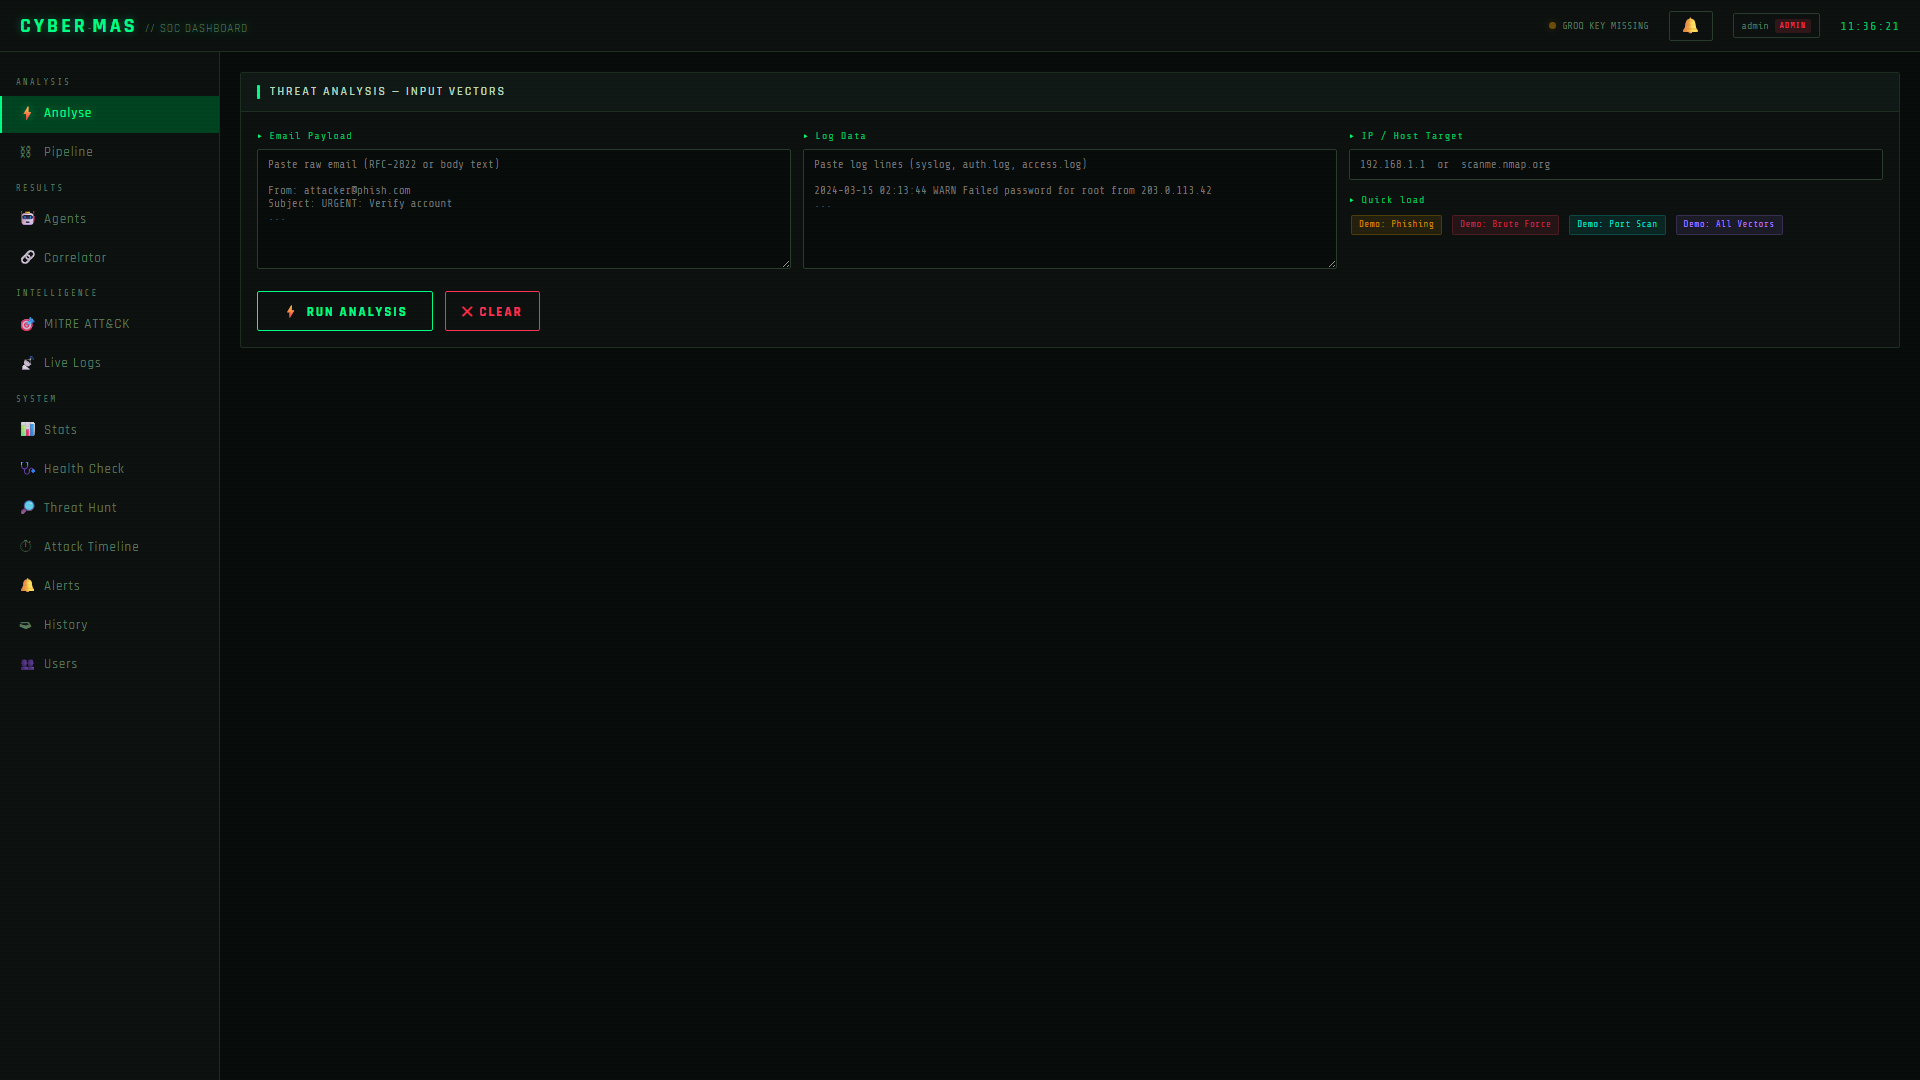
\includegraphics[width=\textwidth]{media/screenshot_analyse.png}
    \caption{Interface principale du Dashboard Cyber-MAS : Panneau d'analyse des vecteurs de menaces.}
    \label{fig:dashboard_analyse}
\end{figure}

\begin{figure}[H]
    \centering
    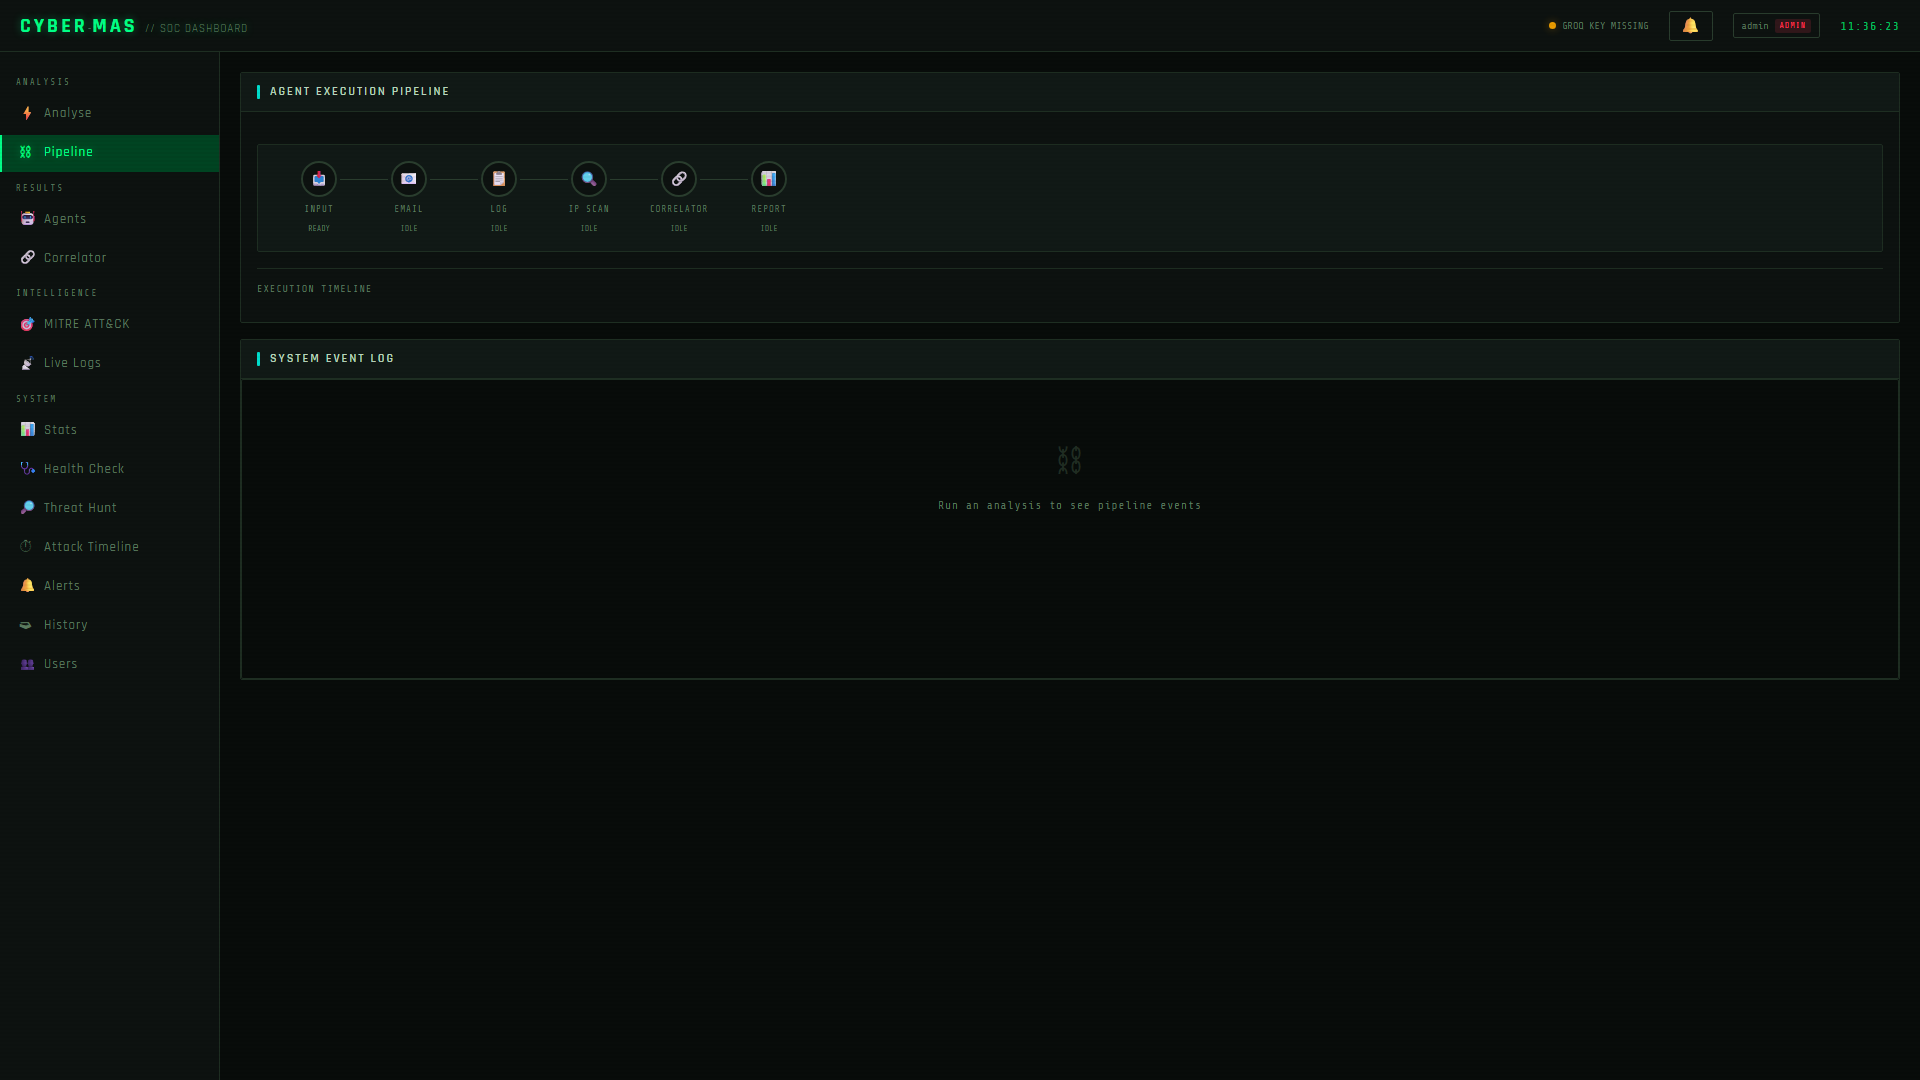
\includegraphics[width=\textwidth]{media/screenshot_pipeline.png}
    \caption{Vue de monitoring du pipeline d'exécution multi-agents en temps réel.}
    \label{fig:dashboard_pipeline}
\end{figure}

\begin{figure}[H]
    \centering
    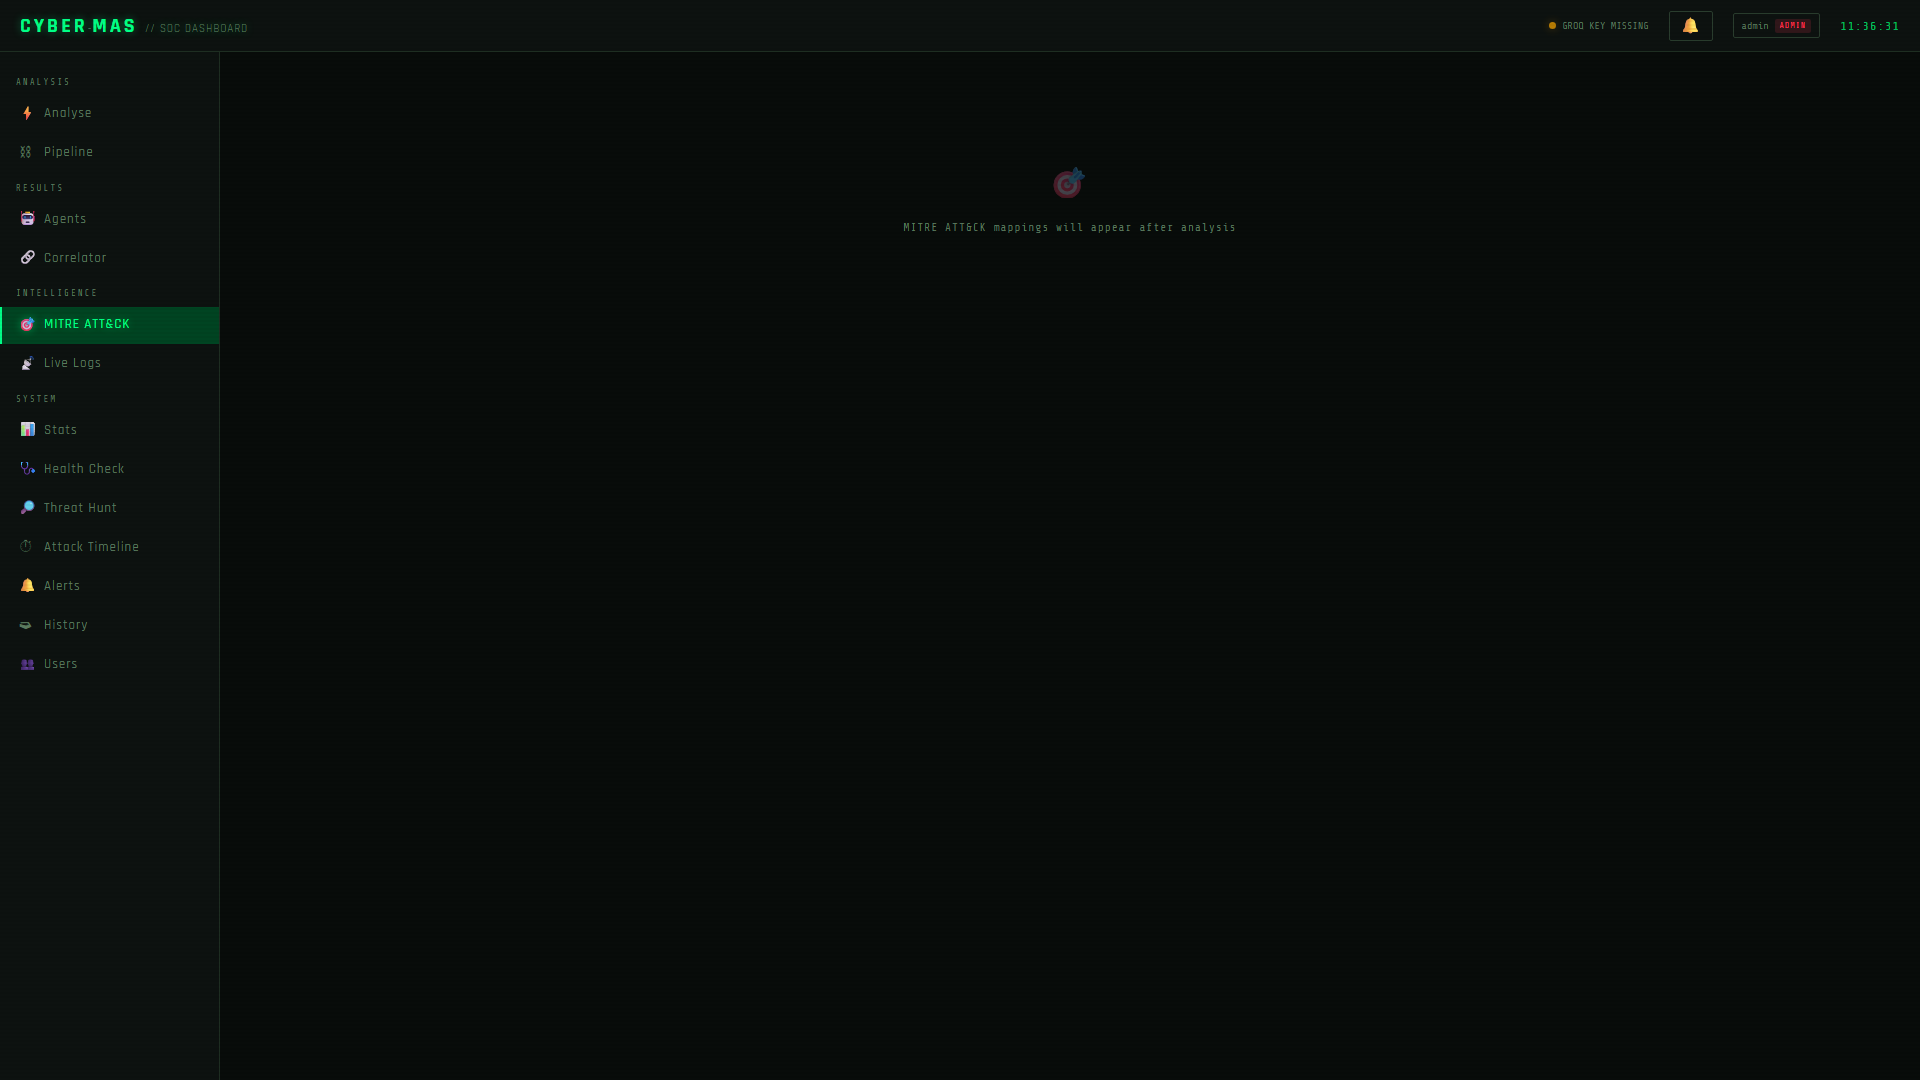
\includegraphics[width=\textwidth]{media/screenshot_mitre.png}
    \caption{Vue de la matrice MITRE ATT\&CK intégrée au Dashboard Cyber-MAS, affichant les tactiques et techniques détectées.}
    \label{fig:dashboard_mitre}
\end{figure}

\begin{figure}[H]
    \centering
    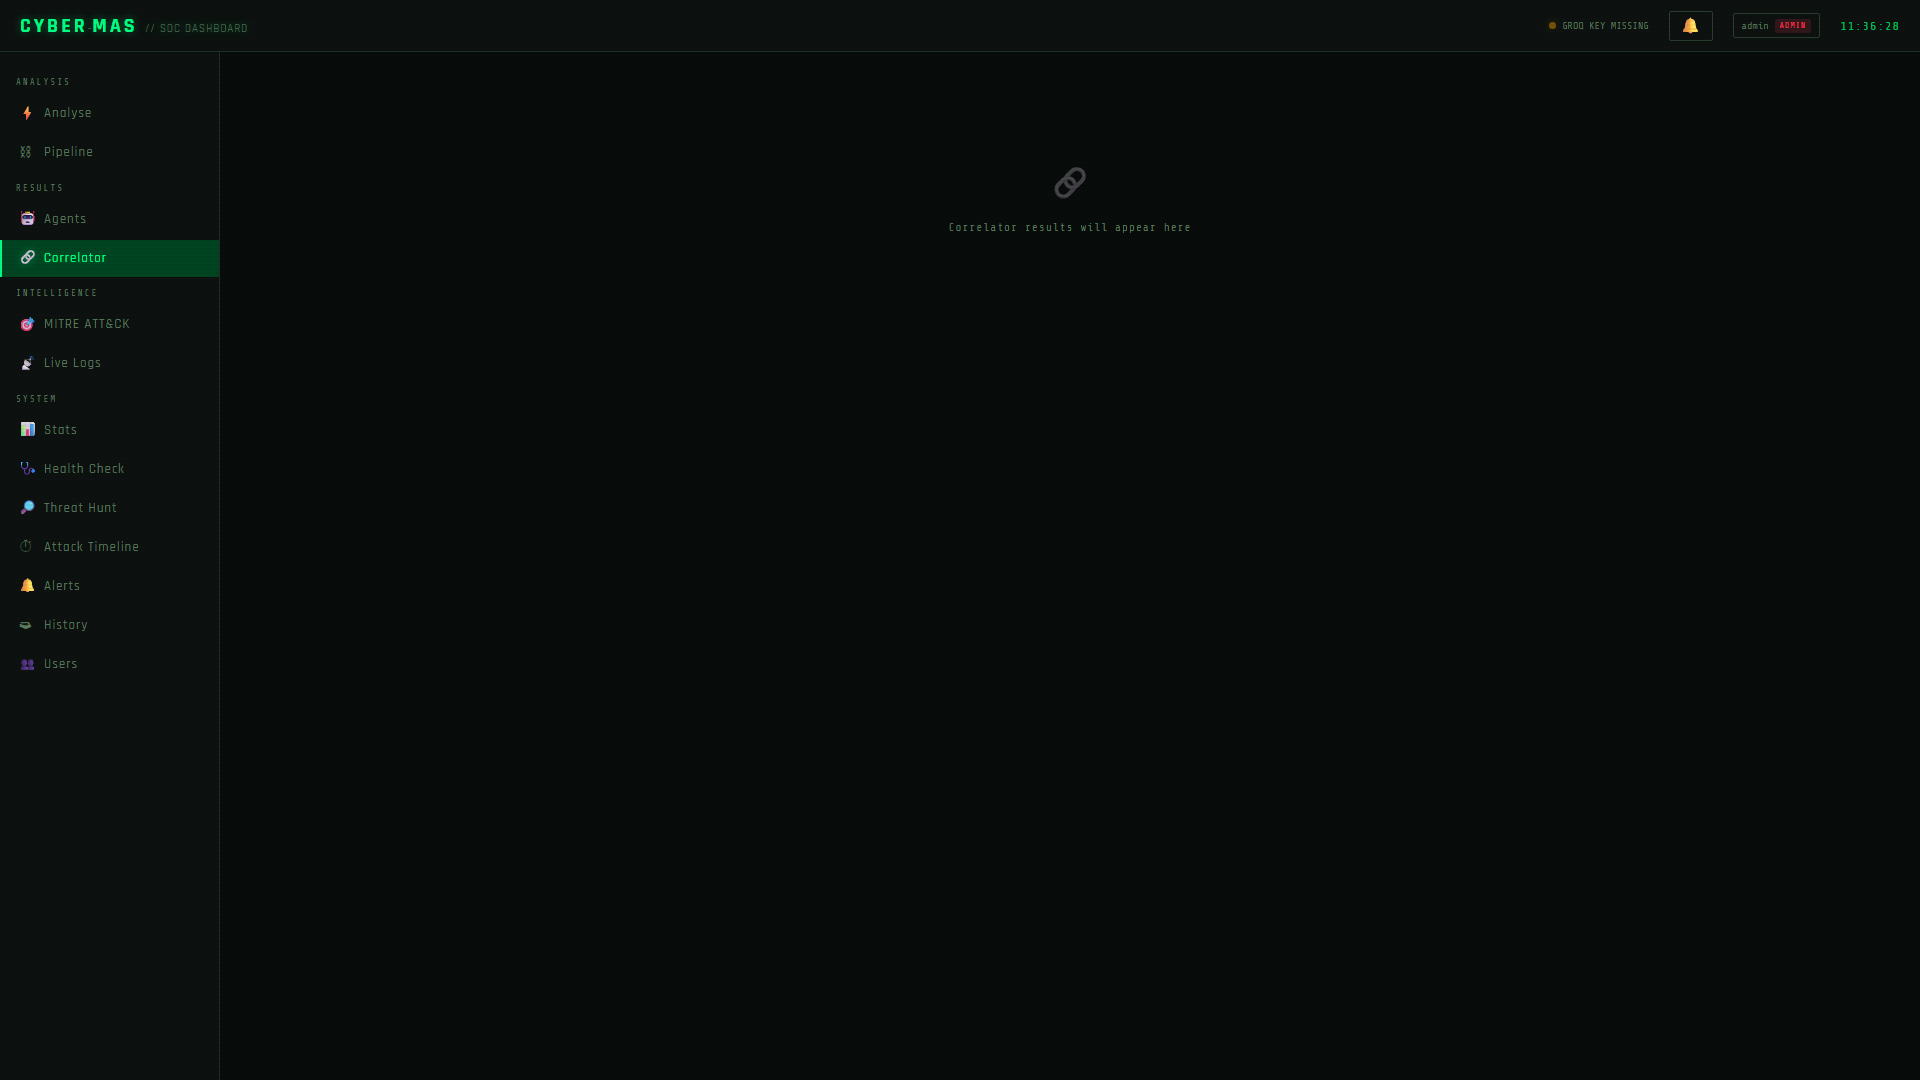
\includegraphics[width=\textwidth]{media/screenshot_correlator.png}
    \caption{Interface de l'Agent Corrélateur, illustrant la fusion sémantique des événements de sécurité.}
    \label{fig:dashboard_correlator}
\end{figure}

\begin{figure}[H]
    \centering
    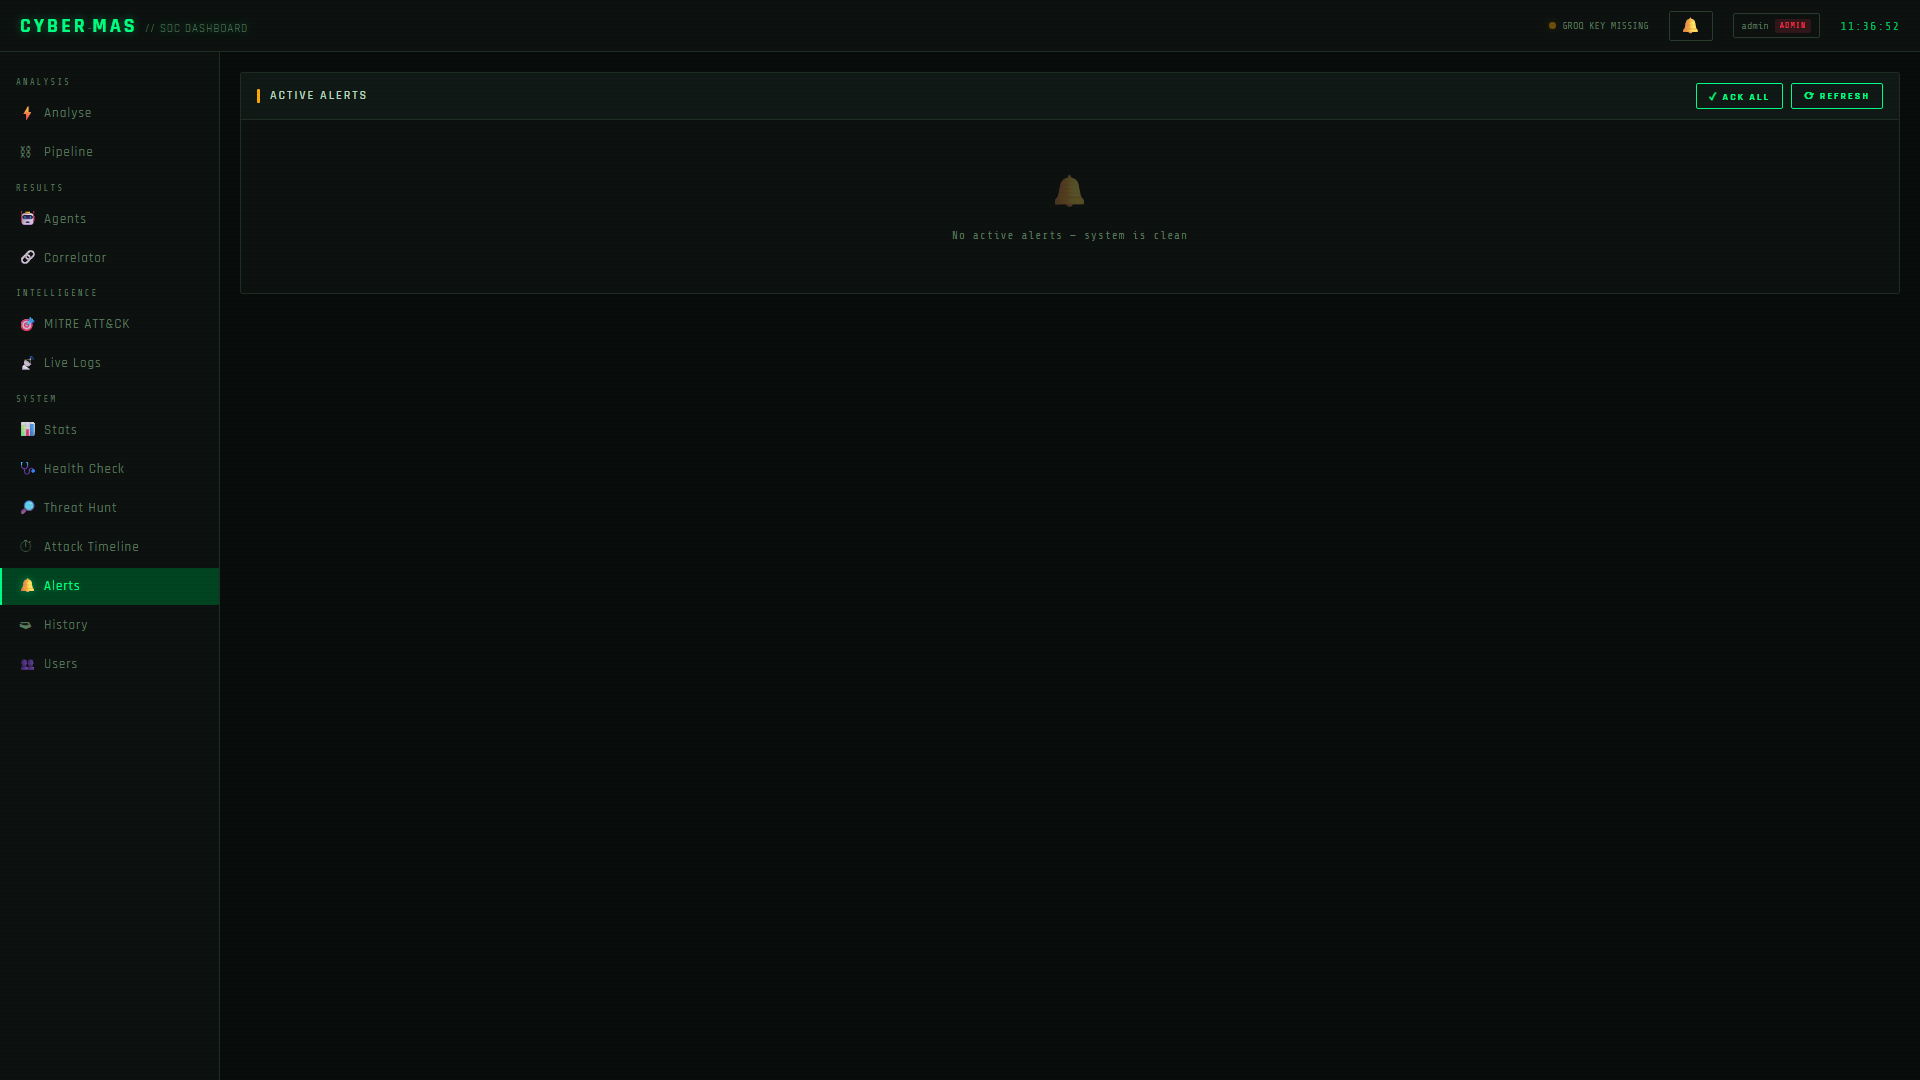
\includegraphics[width=\textwidth]{media/screenshot_alerts.png}
    \caption{Panneau de gestion et de triage des alertes de sécurité pour les analystes SOC.}
    \label{fig:dashboard_alerts}
\end{figure}

\begin{figure}[H]
    \centering
    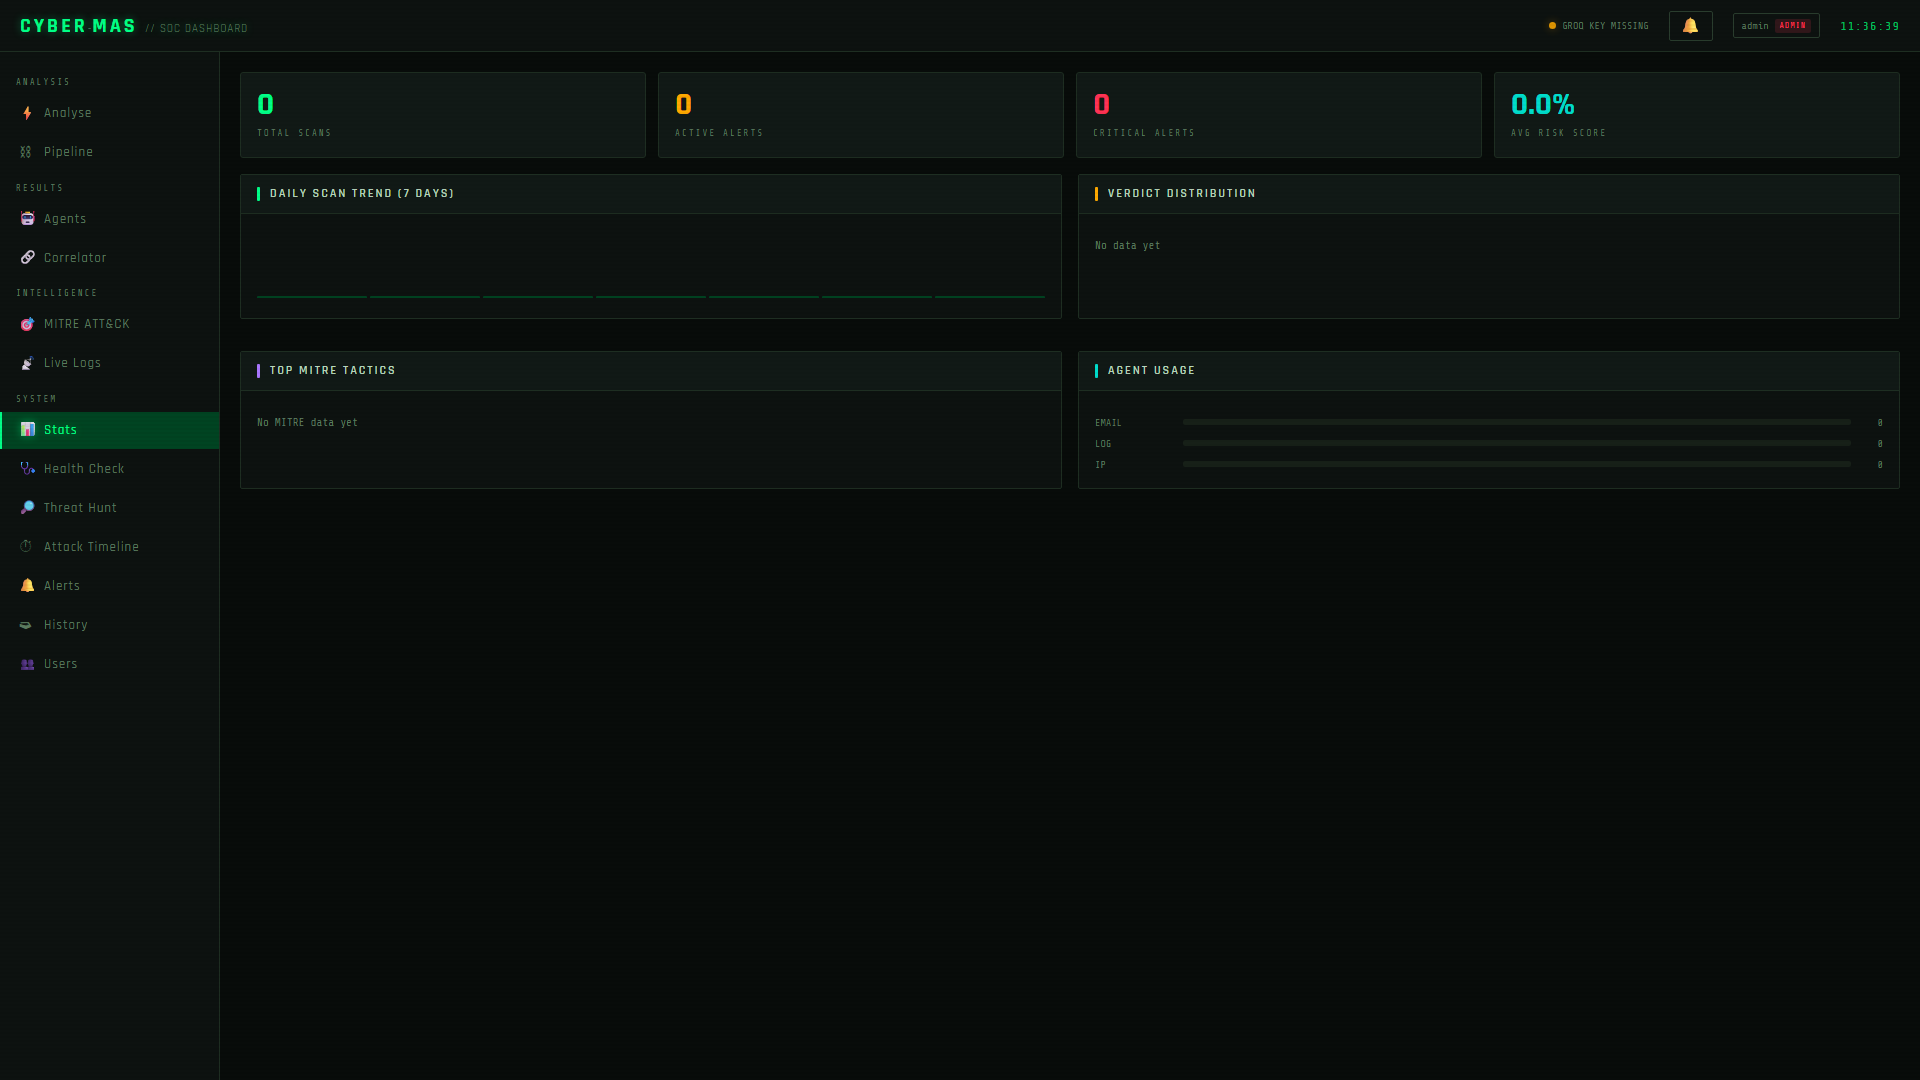
\includegraphics[width=\textwidth]{media/screenshot_stats.png}
    \caption{Tableau de bord des statistiques globales de détection et métriques du système (MTTD, etc.).}
    \label{fig:dashboard_stats}
\end{figure}

\begin{figure}[H]
    \centering
    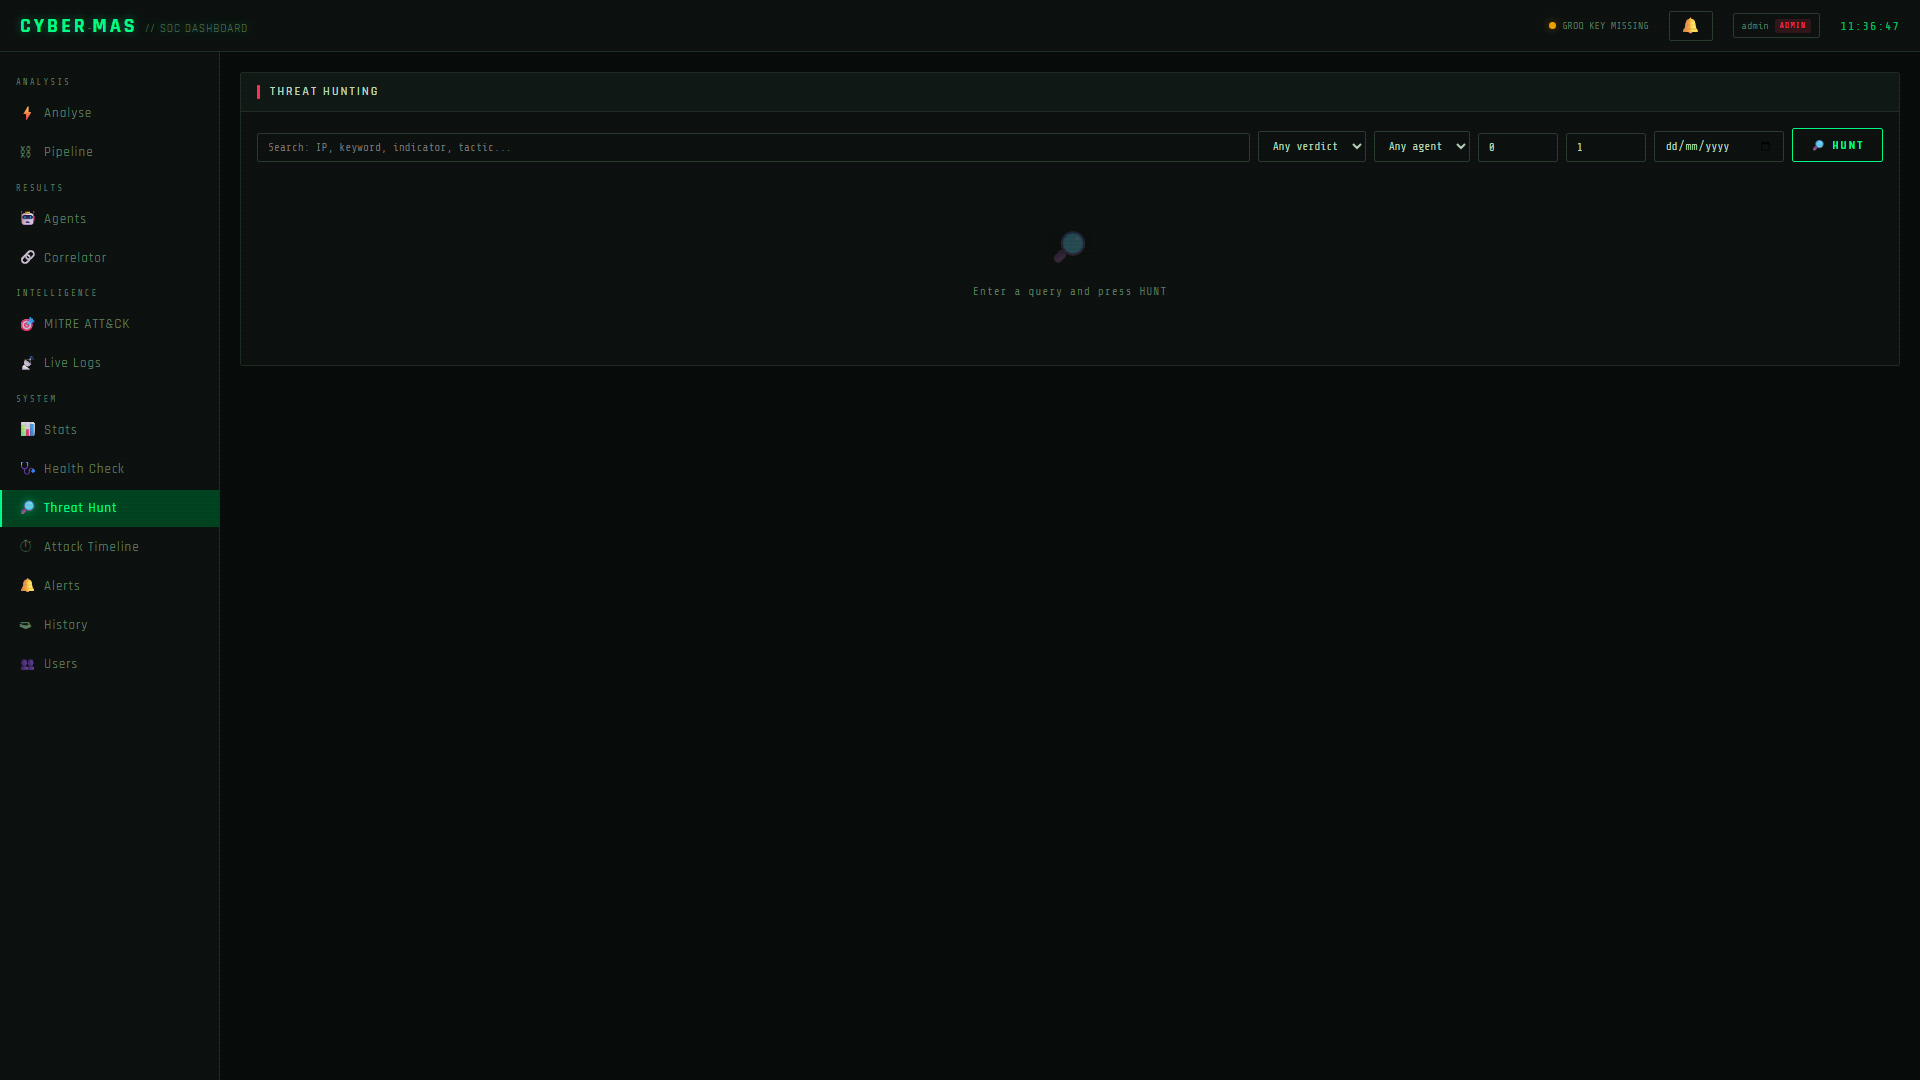
\includegraphics[width=\textwidth]{media/screenshot_hunt.png}
    \caption{Interface de Threat Hunting (Recherche de Menaces) permettant d'interroger la base vectorielle Qdrant.}
    \label{fig:dashboard_hunt}
\end{figure}

\begin{figure}[H]
    \centering
    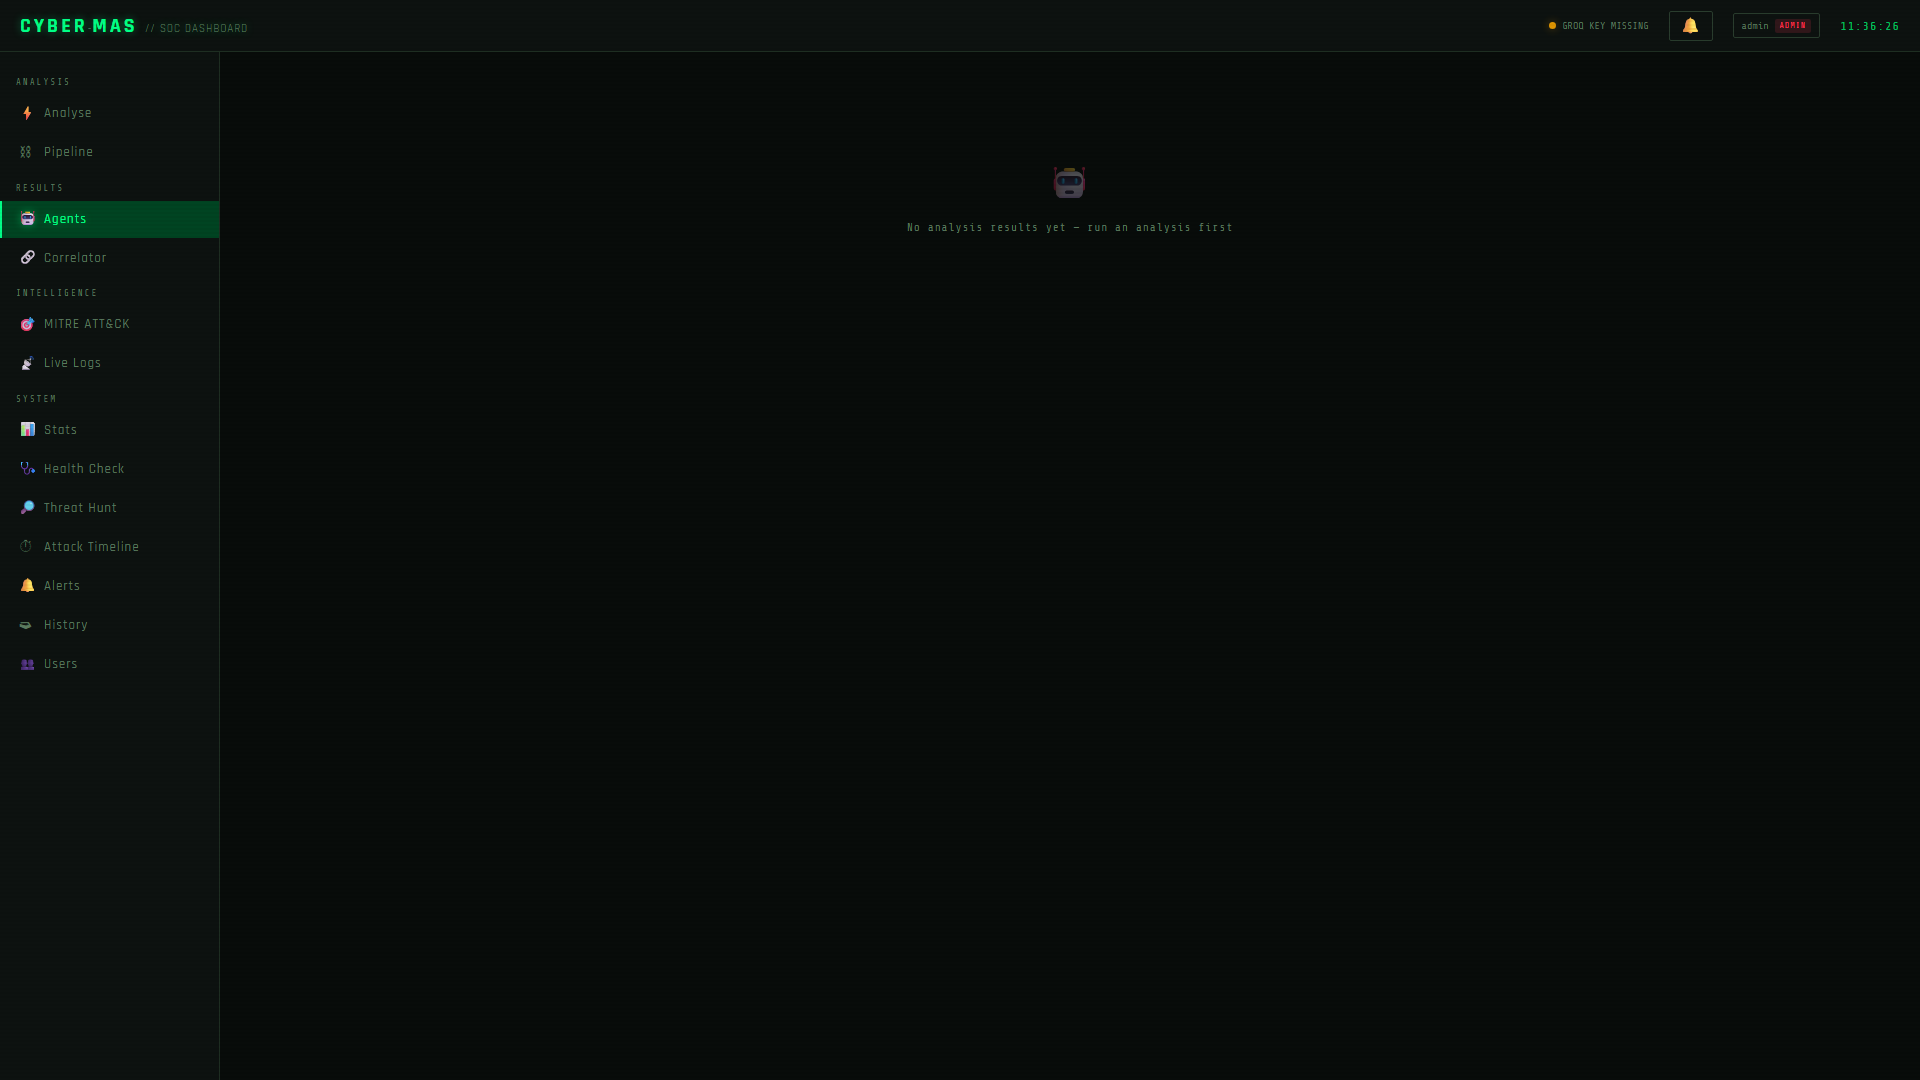
\includegraphics[width=\textwidth]{media/screenshot_agents.png}
    \caption{Vue détaillée de l'état, de la configuration et des journaux individuels des agents LLM.}
    \label{fig:dashboard_agents}
\end{figure}

\subsection{Exécution en mode CLI (Headless)}
Bien que l'interface SOC fournisse une vue d'ensemble complète, Cyber-MAS peut également être exécuté de manière autonome via un terminal (CLI). Ce mode est particulièrement utile pour l'intégration dans des pipelines CI/CD ou pour l'exécution sur des serveurs distants dépourvus d'interface graphique.

\begin{figure}[H]
    \centering
    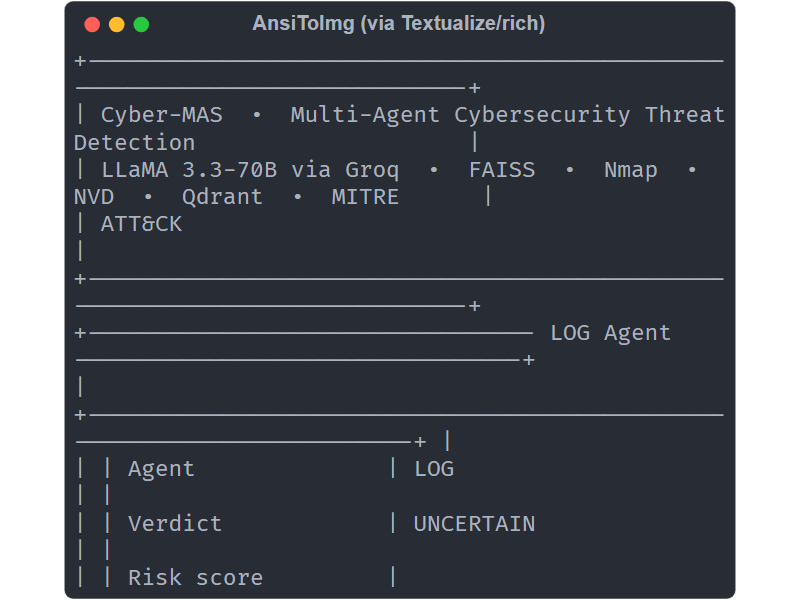
\includegraphics[width=0.9\textwidth]{media/screenshot_cli.png}
    \caption{Exécution de Cyber-MAS en mode console (CLI), affichant le statut de l'analyse et la matrice des résultats.}
    \label{fig:cli_mode}
\end{figure}

\subsection{Génération Automatisée de Rapports}
À l'issue de chaque analyse d'incident, l'Agent Corrélateur compile l'ensemble des données, des traces de raisonnement et des indicateurs de compromission (IoC) pour générer un rapport PDF professionnel. Ce rapport est ensuite distribué automatiquement aux équipes d'intervention pour une remédiation rapide.

\begin{figure}[H]
    \centering
    \fbox{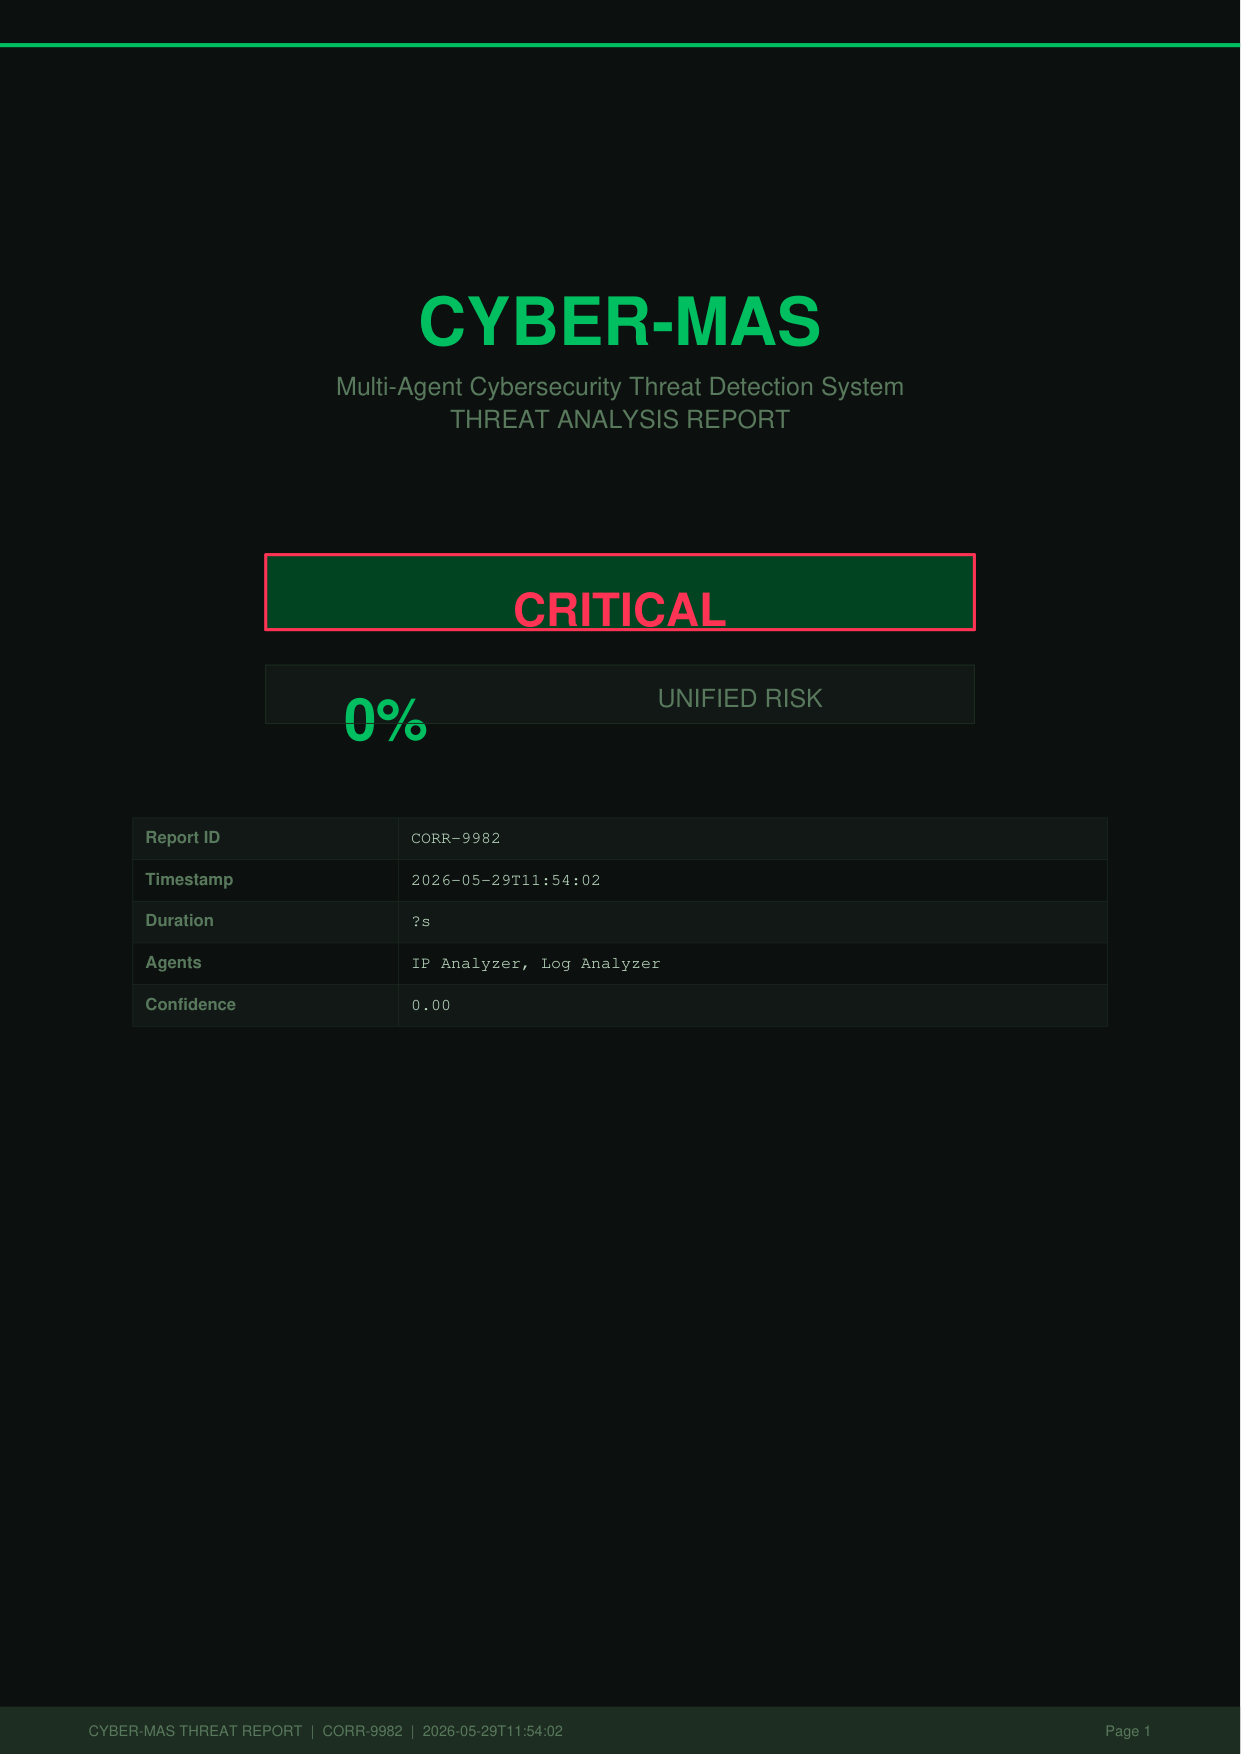
\includegraphics[width=0.8\textwidth]{media/screenshot_pdf.png}}
    \caption{Extrait de la première page d'un rapport d'incident généré automatiquement au format PDF par Cyber-MAS.}
    \label{fig:pdf_report}
\end{figure}

\subsection{Scénario de Validation : Attaque sur calculateur d'infodivertissement}
Afin de valider l'Agent Corrélateur dans un contexte de tests automobiles (bancs HIL), un scénario d'attaque multi-vecteurs a été simulé :
\begin{enumerate}
    \item \textbf{Événement 1 (Agent IP) :} Une adresse IP externe, nouvellement activée et présente dans des listes noires de Botnets, tente d'établir des requêtes vers le réseau de test. L'Agent IP qualifie la menace de modérée.
    \item \textbf{Événement 2 (Agent Log) :} Trente secondes plus tard, un extrait de journal Syslog provenant d'un calculateur d'infodivertissement (ECU) montre une tentative d'authentification SSH non standard ou de mise à jour de firmware (\textit{OTA update}) échouée depuis cette même IP.
\end{enumerate}

\textbf{Résultat observé :} L'Agent Corrélateur a immédiatement intercepté l'intersection des Indicateurs de Compromission (l'adresse IP commune) dans une fenêtre temporelle restreinte. Il a fusionné ces signaux faibles pour générer un Incident Critique, classifié formellement \textit{T1078 - Valid Accounts} selon le MITRE ATT\&CK, déclenchant la génération d'un rapport PDF et l'envoi d'une notification webhook à l'équipe Mécatronique (le détail des logs entrants et des sorties intermédiaires de ce scénario est fourni en Annexe~\ref{annexe:cinematique_donnee}).


Voici un extrait réel de la sortie JSON formatée par le Corrélateur après analyse de l'incident :

\begin{lstlisting}[language=json, basicstyle=\footnotesize\ttfamily]
{
  "alert_id": "CORR-8923",
  "verdict": "critical",
  "risk_score": 0.95,
  "mitre_tactic": "T1078 - Valid Accounts",
  "ioc": ["185.199.108.153"],
  "reasoning": "L'agent IP a identifie l'adresse source comme un point de relais Botnet connu. Simultannement, l'agent Log a remonte des tentatives d'authentification SSH non-standard et un echec critique de deploiment de firmware OTA (ERR_SIGNATURE_MISMATCH) depuis cette IP."
}
\end{lstlisting}


\section{Évaluation des Performances et Indicateurs Clés (KPIs)}
\label{sec:evaluation_performances}

Pour quantifier l'apport opérationnel de Cyber-MAS, le système a été confronté à un jeu de données hybride de sécurité. Les métriques ont été sélectionnées selon les standards d'évaluation SOC recommandés par le SANS Institute \cite{sans_soc_kpi}. Nous avons comparé notre architecture à un pipeline classique (SIEM + Machine Learning de type \textit{Random Forest}).

\subsection{Analyse Comparative des Métriques}
Les résultats, synthétisés dans le Tableau~\ref{tab:kpi_comparison}, démontrent une rupture technologique majeure.


\begin{figure}[H]
    \centering
    \begin{tikzpicture}
        \begin{axis}[
            ybar,
            enlargelimits=0.15,
            legend style={at={(0.5,-0.2)}, anchor=north, legend columns=-1},
            ylabel={Pourcentage (\%)},
            symbolic x coords={Précision, Explicabilité (XAI)},
            xtick=data,
            nodes near coords,
            nodes near coords align={vertical},
            bar width=1.5cm,
            ymin=0, ymax=100
        ]
        \addplot coordinates {(Précision, 78.5) (Explicabilité (XAI), 0)};
        \addplot coordinates {(Précision, 94.2) (Explicabilité (XAI), 100)};
        \legend{SIEM + ML Classique, Cyber-MAS}
        \end{axis}
    \end{tikzpicture}
    \caption{Comparaison graphique de la précision et du taux d'explicabilité entre les systèmes classiques et Cyber-MAS.}
    \label{fig:kpi_chart}
\end{figure}


\begin{table}[htbp]
\centering
\caption{Comparaison des Indicateurs de Performance (KPIs) SOC.}
\label{tab:kpi_comparison}
\vspace{0.2cm}
\begin{tabular}{|l|c|c|p{4cm}|}
\hline
\textbf{Indicateur Clé (KPI)} & \textbf{SIEM + ML Classique} & \textbf{Cyber-MAS} & \textbf{Justification Technique} \\ \hline
\textbf{Précision de Détection} & 78.5 \% & \textbf{94.2 \%} & Le LLM comprend l'intention sémantique, surpassant la simple variance statistique. \\ \hline
\textbf{MTTD (\textit{Mean Time To Detect})} & ~ 2 heures & \textbf{< 1 minute} & Le traitement asynchrone et distribué des agents élimine les goulots d'indexation. \\ \hline
\textbf{Taux d'Explicabilité (XAI)} & 0 \% (\textit{Boîte Noire}) & \textbf{100 \%} & Génération systématique d'un rapport en langage naturel justifiant la décision. \\ \hline
\end{tabular}
\end{table}

\subsection{Validation de la boucle d'apprentissage (Baisse du FPR)}
L'impact du mécanisme \textit{In-Context Learning} a été empiriquement mesuré. Lors du premier passage du jeu de données, des routines de diagnostic régulières de l'infrastructure ont été signalées à tort (Taux de Faux Positifs de 8.5 \%). 
Après signalement de ces événements via l'interface, le module de rétroaction a mis à jour le RAG. Lors du second passage, le LLM a intégré cette directive locale, faisant chuter le Taux de Faux Positifs (FPR) à \textbf{3.1 \%}. Ce résultat valide la capacité du système à s'adapter à l'environnement spécifique de l'équipe Validation OTA sans nécessiter de réentraînement algorithmique coûteux.

\begin{table}[htbp]
\centering
\caption{Impact de l'In-Context Learning (RAG) sur la réduction de la fatigue d'alerte}
\label{tab:resultats_rag}
\vspace{0.2cm}
\begin{tabular}{|p{4.5cm}|c|c|c|}
\hline
\textbf{Scénario de test (Banc HIL)} & \textbf{FPR (Sans RAG)} & \textbf{FPR (Avec RAG)} & \textbf{Gain Opérationnel} \\ \hline
\textbf{Trafic normal (Bruit de fond)} & 2.4 \% & 0.8 \% & Diminution des micro-alertes \\ \hline
\textbf{Scans de vulnérabilité internes} & 18.5 \% & 4.2 \% & Excellente assimilation du contexte \\ \hline
\textbf{Mises à jour OTA légitimes} & 8.5 \% & \textbf{3.1 \%} & Réduction drastique des faux positifs majeurs \\ \hline
\end{tabular}
\end{table}

\begin{figure}[H]
    \centering
    \begin{tikzpicture}
        \begin{axis}[
            ybar,
            enlargelimits=0.15,
            legend style={at={(0.5,-0.25)}, anchor=north, legend columns=-1},
            ylabel={Taux de Faux Positifs (\%)},
            symbolic x coords={Trafic normal, Scans internes, MAJ OTA},
            xtick=data,
            nodes near coords,
            nodes near coords align={vertical},
            bar width=1.2cm,
            ymin=0, ymax=22
        ]
        \addplot[fill=red!60] coordinates {(Trafic normal, 2.4) (Scans internes, 18.5) (MAJ OTA, 8.5)};
        \addplot[fill=green!60] coordinates {(Trafic normal, 0.8) (Scans internes, 4.2) (MAJ OTA, 3.1)};
        \legend{Sans RAG, Avec RAG}
        \end{axis}
    \end{tikzpicture}
    \caption{Impact de la boucle d'apprentissage RAG sur la r\'eduction du Taux de Faux Positifs (FPR) par sc\'enario de test sur banc HIL.}
    \label{fig:fpr_rag_chart}
\end{figure}

\section*{Conclusion}
\addcontentsline{toc}{section}{Conclusion}
Cette phase de réalisation valide la viabilité technique et opérationnelle de l'architecture Cyber-MAS. L'implémentation a démontré la faisabilité d'un réseau asynchrone performant où des agents cognitifs interagissent pour qualifier une menace complexe. Les tests en contexte applicatif (infodivertissement automobile) et l'évaluation sur des KPIs standardisés prouvent que cette hybridation MAS/LLM surpasse les solutions de détection centralisées opaques. En offrant une détection quasi-instantanée, une précision supérieure à 94\% et une explicabilité totale (XAI), le système répond intégralement au cahier des charges initial, soulageant efficacement la charge cognitive des ingénieurs de validation et sécurisant les cycles de test des véhicules connectés.

\chapter*{Conclusion Générale}
\addcontentsline{toc}{chapter}{Conclusion Générale}

L'accélération de la numérisation dans l'industrie automobile a transformé les véhicules en véritables écosystèmes cyber-physiques \cite{ibm_report}. Si cette évolution offre des fonctionnalités de pointe, elle expose également les systèmes embarqués à des menaces informatiques d'une complexité inédite, régies par des normes de validation strictes telles que l'ISO/SAE 21434 \cite{iso_21434}. Au sein du département \textit{Product \& Systems Engineering} de Capgemini Engineering, ce Projet de Fin d'Études ambitionnait de résoudre une problématique de l'équipe Validation OTA : l'incapacité des systèmes de détection traditionnels à corréler des attaques multi-vecteurs \cite{cisco_trends} et l'opacité sémantique du Machine Learning classique, générateurs d'une dangereuse « fatigue d'alerte » \cite{hassan_alert_fatigue}.

Pour répondre à ce défi industriel, nous avons conçu et développé \textbf{Cyber-MAS}, une architecture de cybersécurité de nouvelle génération. Ce projet a démontré avec succès que l'hybridation entre l'Intelligence Artificielle Distribuée \cite{wooldridge_mas} et la puissance sémantique des Grands Modèles de Langage \cite{openai_gpt4} constitue une réponse robuste aux Menaces Persistantes Avancées (APT). 

Tout au long de ce projet, nous avons validé notre démarche d'ingénierie :
\begin{itemize}
    \item \textbf{Décentralisation :} L'instanciation d'agents autonomes (Log, IP, Email) a permis un traitement asynchrone hautement scalable \cite{kotkar_mas}.
    \item \textbf{Corrélation :} L'Agent Corrélateur a prouvé sa capacité à fusionner des signaux faibles spatio-temporels et à les standardiser sur la matrice MITRE ATT\&CK \cite{mitre_attack}.
    \item \textbf{Apprentissage Continu :} L'intégration du paradigme RAG \cite{lewis_rag} via une mémoire vectorielle a doté le système d'un \textit{In-Context Learning} \cite{dong_icl}, faisant chuter le taux de faux positifs à 3.1\%.
    \item \textbf{Transparence (XAI) :} L'IA Explicable \cite{darpa_xai} a transformé des scores obscurs en rapports factuels, atteignant une précision de détection de 94.2\% et un MTTD inférieur à une minute \cite{sans_soc_kpi}.
\end{itemize}

Bien que le système réponde pleinement au cahier des charges, ce travail ouvre plusieurs perspectives d'évolution :
\begin{enumerate}
    \item \textbf{Souveraineté (Local LLMs) :} L'intégration de modèles quantifiés hébergés localement permettrait un cloisonnement absolu des données de validation.
    \item \textbf{Réponse Active (SOAR) :} Doter les agents de capacités d'action pour isoler automatiquement un calculateur (ECU) d'infodivertissement compromis.
    \item \textbf{Agent CAN Bus :} Le développement d'un agent spécialisé dans l'analyse comportementale des protocoles matériels spécifiques à l'automobile.
\end{enumerate}

En définitive, ce projet a constitué une expérience d'ingénierie très riche, alliant recherche scientifique et exigences industrielles. Cyber-MAS prouve que la transparence et la distribution cognitive façonneront l'avenir de la cyberdéfense.

\begin{thebibliography}{99}
\addcontentsline{toc}{chapter}{Bibliographie}

% ==========================================
% PAPIERS SCIENTIFIQUES & RECHERCHE (IA, MAS, XAI)
% ==========================================

\bibitem{lewis_rag}
P. Lewis \textit{et al.}, ``Retrieval-Augmented Generation for Knowledge-Intensive NLP Tasks,'' \textit{Advances in Neural Information Processing Systems (NeurIPS)}, vol. 33, pp. 9459-9474, 2020.

\bibitem{wei_cot}
J. Wei \textit{et al.}, ``Chain-of-Thought Prompting Elicits Reasoning in Large Language Models,'' \textit{Advances in Neural Information Processing Systems (NeurIPS)}, vol. 35, pp. 24824-24837, 2022.

\bibitem{wooldridge_mas}
M. Wooldridge et N. R. Jennings, ``Intelligent Agents: Theory and Practice,'' \textit{The Knowledge Engineering Review}, vol. 10, no. 2, pp. 115-152, 1995.

\bibitem{kotkar_mas}
D. B. Kotkar \textit{et al.}, ``A review of multi-agent system applied to intrusion detection system,'' \textit{International Journal of Computer Applications}, 2015.

\bibitem{aminanto_xai}
M. E. Aminanto \textit{et al.}, ``Deep Learning in Intrusion Detection Systems: A Review and Explainability perspective,'' \textit{IEEE Access}, 2023.

\bibitem{dong_icl}
Q. Dong \textit{et al.}, ``A Survey on In-context Learning,'' \textit{arXiv preprint arXiv:2301.00234}, 2023.

\bibitem{darpa_xai}
D. Gunning et D. Aha, ``DARPA’s Explainable Artificial Intelligence (XAI) Program,'' \textit{AI Magazine}, vol. 40, no. 2, pp. 44-58, 2019.

\bibitem{hassan_alert_fatigue}
W. U. Hassan \textit{et al.}, ``Tactical Provenance Analysis for Endpoint Detection and Response Systems,'' \textit{IEEE Symposium on Security and Privacy (SP)}, pp. 1171-1189, 2020.

\bibitem{faiss_paper}
J. Johnson, M. Douze, et H. Jégou, ``Billion-scale similarity search with GPUs,'' \textit{IEEE Transactions on Big Data}, vol. 7, no. 3, pp. 535-547, 2019.

\bibitem{openai_gpt4}
Meta AI, ``Llama 3 Herd of Models,'' \textit{arXiv preprint arXiv:2407.21783}, 2024.

% ==========================================
% NORMES, FRAMEWORKS & STANDARDS INDUSTRIELS
% ==========================================

\bibitem{iso_21434}
ISO/SAE 21434:2021, ``Road vehicles — Cybersecurity engineering,'' Organisation Internationale de Normalisation, 2021.

\bibitem{mitre_attack}
The MITRE Corporation, ``MITRE ATT\&CK Framework,'' 2026. [En ligne]. Disponible: \url{https://attack.mitre.org}.

\bibitem{nist_nvd}
National Institute of Standards and Technology (NIST), ``National Vulnerability Database (NVD) API Documentation,'' 2026. [En ligne]. Disponible: \url{https://nvd.nist.gov/}.

\bibitem{w3c_sse}
World Wide Web Consortium (W3C), ``Server-Sent Events - W3C Recommendation,'' 2015. [En ligne]. Disponible: \url{https://www.w3.org/TR/eventsource/}.

% ==========================================
% TECHNOLOGIES, DOCUMENTATIONS & OUTILS
% ==========================================

\bibitem{fastapi}
S. Ramírez, ``FastAPI Documentation - High performance, easy to learn, fast to code, ready for production,'' 2026. [En ligne]. Disponible: \url{https://fastapi.tiangolo.com/}.

\bibitem{qdrant}
Qdrant, ``Qdrant - High-performance, massive-scale Vector Database,'' 2026. [En ligne]. Disponible: \url{https://qdrant.tech/documentation/}.

\bibitem{suricata_oisf}
Open Information Security Foundation (OISF), ``Suricata User Guide,'' 2026. [En ligne]. Disponible: \url{https://suricata.io/}.

\bibitem{openai_api}
Groq, ``Groq API Documentation,'' 2026. [En ligne]. Disponible: \url{https://console.groq.com/docs/}.

% ==========================================
% RAPPORTS DE L'INDUSTRIE (SOC & MENACES)
% ==========================================

\bibitem{ibm_report}
IBM Security, ``Cost of a Data Breach Report 2024,'' IBM Corporation, 2024. [En ligne]. Disponible: \url{https://www.ibm.com/reports/data-breach}.

\bibitem{cisco_trends}
Cisco, ``Cybersecurity Threat Trends: Phishing, Ransomware, and Multi-vector Attacks,'' Cisco Systems, 2024. [En ligne]. Disponible: \url{https://www.cisco.com/c/en/us/products/security/threat-intelligence.html}.

\bibitem{sans_soc_kpi}
SANS Institute, ``Metrics for Security Operations Centers (SOC): What to Measure and Why,'' SANS Reading Room, 2021. [En ligne]. Disponible: \url{https://www.sans.org/reading-room/}.

\end{thebibliography}

% =====================================================================
%              LISTE DES ABREVIATIONS
% =====================================================================
\newpage
\chapter*{Liste des Abréviations}
\addcontentsline{toc}{chapter}{Liste des Abréviations}

\begin{tabular}{ll}
\textbf{API} & Application Programming Interface \\
\textbf{APT} & Advanced Persistent Threat \\
\textbf{CAN} & Controller Area Network \\
\textbf{CTI} & Cyber Threat Intelligence \\
\textbf{CVE} & Common Vulnerabilities and Exposures \\
\textbf{ECU} & Electronic Control Unit \\
\textbf{HIL} & Hardware In the Loop \\
\textbf{IDS} & Intrusion Detection System \\
\textbf{LLM} & Large Language Model \\
\textbf{MAS} & Multi-Agent System \\
\textbf{ML} & Machine Learning \\
\textbf{OTA} & Over-The-Air \\
\textbf{RAG} & Retrieval-Augmented Generation \\
\textbf{SIEM} & Security Information and Event Management \\
\textbf{SOC} & Security Operations Center \\
\textbf{XAI} & Explainable Artificial Intelligence \\
\end{tabular}


% ==========================================
% DÉBUT DES ANNEXES
% ==========================================
\appendix
\addcontentsline{toc}{part}{Annexes}

\chapter{Ingénierie de Prompt (Prompt Engineering)}
\label{annexe:prompt_engineering}

Cette annexe détaille la structure cognitive imposée au Grand Modèle de Langage (LLM). Pour garantir des résultats déterministes et explicables (XAI) dans le contexte critique de la cybersécurité automobile, le modèle n'est pas interrogé librement. Il est contraint par un cadre strict divisé en trois composantes.

\section{A.1. Le "System Prompt" : Rôle et Contexte}
La première étape consiste à définir le rôle de l'IA et le contexte opérationnel. Cela permet d'éliminer les hallucinations en forçant le modèle à se concentrer uniquement sur le domaine de la validation embarquée.

\vspace{0.3cm}
\noindent\begin{minipage}{\linewidth}
\begin{lstlisting}[basicstyle=\footnotesize\ttfamily, breaklines=true, caption={Définition du rôle et du contexte industriel.}]
SYSTEM_PROMPT = """
You are an expert Automotive SOC Analyst specializing in Over-The-Air (OTA) update validation and ECU security.
Your mission is to analyze telemetry data and agent reports from a Stellantis HIL test bench.
You must identify anomalies such as Downgrade Attacks, Man-in-the-Middle (MitM), or unauthorized firmware flashing.
Do not make assumptions outside of the provided data.
"""
\end{lstlisting}
\end{minipage}

\section{A.2. La technique du "Chain of Thought" (CoT)}
Pour obtenir la composante d'Intelligence Artificielle Explicable (XAI), nous obligeons le modèle à détailler son raisonnement logique \textit{avant} de formuler son verdict final. 

\vspace{0.3cm}
\noindent\begin{minipage}{\linewidth}
\begin{lstlisting}[basicstyle=\footnotesize\ttfamily, breaklines=true, caption={Directive forçant le raisonnement par étapes (Chain of Thought).}]
COT_DIRECTIVE = """
Before providing your final verdict, you must think step-by-step.
1. Analyze the IP reputation report. Is the source a known OEM server?
2. Analyze the ECU logs. Are there cryptographic signature mismatches?
3. Correlate the two: Does this indicate a targeted attack on the OTA pipeline?
Write your detailed explanation in French in the 'reasoning' field.
"""
\end{lstlisting}
\end{minipage}

\section{A.3. Formatage de sortie (Output Parsing)}
Afin que les données générées par le LLM puissent être ingérées par le Dashboard SOC, une directive de formatage strict est appliquée. Le modèle est pénalisé s'il génère du texte en dehors de la structure JSON demandée.

\vspace{0.3cm}
\noindent\begin{minipage}{\linewidth}
\begin{lstlisting}[basicstyle=\footnotesize\ttfamily, breaklines=true, caption={Contrainte syntaxique pour la génération de JSON pur.}]
FORMAT_INSTRUCTIONS = """
Your final output MUST be a valid, raw JSON object. Do not wrap it in Markdown formatting (no ```json).
Adhere strictly to this schema:
{
  "verdict": "malicious" | "suspicious" | "safe",
  "risk_score": <float between 0.0 and 1.0>,
  "mitre_tactic": "<String: Tactic ID and Name>",
  "ioc": ["<List of IP addresses or Hashes>"],
  "reasoning": "<String: Your step-by-step XAI explanation in French>"
}
"""
\end{lstlisting}
\end{minipage}


\chapter{Extraits de Code : Architecture Système Cyber-MAS}
\label{annexe:architecture_code}

Cette annexe met en évidence les composants logiciels critiques développés en Python (framework FastAPI). L'architecture favorise la modularité orientée objet, où chaque agent et chaque outil possède un rôle strictement délimité.

\section{B.1. Les Agents Cognitifs (Système Multi-Agents)}

L'approche MAS (Multi-Agent System) repose sur la spécialisation. Au lieu d'avoir un script monolithique, la donnée est traitée par des agents experts indépendants.

\subsection{B.1.1. L'Agent Log (Analyseur de trames ECU)}
Le rôle de cet agent est de parser les fichiers journaux bruts provenant des calculateurs (par exemple, le TCU - Telematics Control Unit) lors d'une tentative de mise à jour OTA. Il recherche spécifiquement des anomalies de format ou des codes d'erreur internes (comme des erreurs de signature cryptographique).

\vspace{0.3cm}
\noindent\begin{minipage}{\linewidth}
\begin{lstlisting}[language=Python, basicstyle=\footnotesize\ttfamily, breaklines=true, caption={Extraction et analyse des codes d'erreur par l'Agent Log.}]
async def analyse_logs(log_text: str) -> dict:
    # Extrait de agents/log_agent.py
    log.info("Log Agent starting analysis...")
    lines = [ln.strip() for ln in log_text.splitlines() if ln.strip()]
    if not lines:
        return _error_result("empty_input", 0.0, "No valid log lines provided.")

    sys_prompt = prompts.log_system_prompt()
    usr_prompt = prompts.log_user_prompt("\n".join(lines), "")

    try:
        reply = ask(sys_prompt, usr_prompt, max_tokens=1500)
        parsed = _parse_llm_json(reply)
        parsed["agent"] = "log"
        return parsed
    except Exception as e:
        log.error(f"Log Agent LLM error: {e}")
        return _error_result("llm_error", 0.0, str(e))
\end{lstlisting}
\end{minipage}

\subsection{B.1.2. L'Agent IP (Analyseur de réputation réseau)}
Cet agent se concentre uniquement sur les métadonnées réseau. Lorsqu'une mise à jour OTA est initiée, l'Agent IP isole l'adresse source et vérifie si le véhicule communique avec un serveur cloud légitime ou avec un serveur pirate (attaque Man-in-the-Middle).

\vspace{0.3cm}
\noindent\begin{minipage}{\linewidth}
\begin{lstlisting}[language=Python, basicstyle=\footnotesize\ttfamily, breaklines=true, caption={Analyse de l'adresse source par l'Agent IP.}]
async def analyse_ip(target: str) -> dict:
    # Extrait de agents/ip_agent.py
    log.info(f"IP Agent starting analysis for target: {target}")
    if not target:
        return _error_result("missing_target", "No IP/Host provided.")

    ip_data = check_ip_reputation(target)
    sys_prompt = prompts.ip_system_prompt()
    usr_prompt = prompts.ip_user_prompt(
        target=target,
        is_valid_ip=ip_data["is_valid_ip"],
        is_private=ip_data["is_private"],
        open_ports=ip_data["open_ports"],
        cves=ip_data["cves"]
    )

    try:
        reply = ask(sys_prompt, usr_prompt)
        parsed = _parse_llm_json(reply)
        parsed["agent"] = "ip"
        return parsed
    except Exception as e:
        return _error_result("llm_error", str(e))
\end{lstlisting}
\end{minipage}

\subsection{B.1.3. L'Agent Corrélateur (Fusion et LLM)}
C'est le chef d'orchestre. Il ne lit pas les logs bruts. Il attend que les Agents Log et IP aient terminé leur travail, rassemble leurs rapports JSON, interroge la mémoire (RAG) et envoie le tout au LLM pour prendre la décision finale.

\vspace{0.3cm}
\noindent\begin{minipage}{\linewidth}
\begin{lstlisting}[language=Python, basicstyle=\footnotesize\ttfamily, breaklines=true, caption={Fusion des donnees et appel au LLM par le Correlateur.}]
class AgentCorrelateur(BaseAgent):
    async def fuse_and_evaluate(self, agent_results: list) -> dict:
        # 1. Recuperation du contexte historique via RAG
        historical_context = tool_rag_memory.search(str(agent_results))
        
        # 2. Construction du prompt final
        final_prompt = f"""
        Resultats des agents : {agent_results}
        Contexte historique (Faux positifs OTA) : {historical_context}
        """
        
        # 3. Appel securise au Grand Modele de Langage
        xai_decision = await safe_llm_call(SYSTEM_PROMPT + final_prompt)
        return xai_decision
\end{lstlisting}
\end{minipage}

\section{B.2. Les Outils Externes (Tools \& APIs)}

Les outils sont des fonctions utilitaires passives. Contrairement aux agents (qui prennent des décisions), les outils se contentent de fournir de la donnée brute lorsqu'ils sont sollicités.

\subsection{B.2.1. Outil de Mémoire Vectorielle (RAG)}
Cet outil encapsule la logique de connexion à la base de données vectorielle (FAISS ou Qdrant). Il transforme les requêtes textuelles en vecteurs pour retrouver des incidents similaires du passé.

\vspace{0.3cm}
\noindent\begin{minipage}{\linewidth}
\begin{lstlisting}[language=Python, basicstyle=\footnotesize\ttfamily, breaklines=true, caption={Outil RAG pour l'apprentissage en contexte.}]
def query_memory(query_text: str, limit: int = 3) -> list[MemoryMatch]:
    # Extrait de tools/qdrant_store.py
    client = _get_client()
    if not client: return []
    try:
        vec = _get_embedding(query_text)
        hits = client.search(
            collection_name=COLLECTION_NAME,
            query_vector=vec,
            limit=limit,
            score_threshold=0.75
        )
        return [MemoryMatch(
            similarity=h.score,
            agent_type=h.payload.get("agent_type", "unknown"),
            verdict=h.payload.get("verdict", "unknown"),
            risk_score=h.payload.get("risk_score", 0.0)
        ) for h in hits]
    except Exception as e:
        return []
\end{lstlisting}
\end{minipage}

\subsection{B.2.2. Outil de Threat Intelligence (CTI)}
Cet outil permet à l'architecture de vérifier des informations réseau externes. Dans notre contexte, il vérifie si une adresse IP appartient bien à l'infrastructure officielle de mise à jour du constructeur.

\vspace{0.3cm}
\noindent\begin{minipage}{\linewidth}
\begin{lstlisting}[language=Python, basicstyle=\footnotesize\ttfamily, breaklines=true, caption={Outil d'interrogation des bases de reputation reseau.}]
class ToolThreatIntel:
    async def check_ip(self, ip: str) -> dict:
        # Simulation d'une requete vers une API de Threat Intel ou une liste blanche OEM
        known_oem_ips = ["192.168.100.5", "10.0.0.8"] # Exemple de serveurs OTA legitimes
        
        if ip in known_oem_ips:
            return {"reputation": "safe", "belongs_to_oem": True}
        else:
            # Appel hypothetique a une API (ex: VirusTotal)
            api_result = await http_client.get(f"https://threat-api.com/ip/{ip}")
            return {"reputation": "suspicious", "belongs_to_oem": False}
\end{lstlisting}
\end{minipage}

\section{B.3. Mode Continu (Continuous Monitoring)}
Pour assurer une surveillance en temps réel sans intervention humaine, un processus asynchrone surveille en boucle le pipeline de logs généré par les calculateurs.

\vspace{0.3cm}
\noindent\begin{minipage}{\linewidth}
\begin{lstlisting}[language=Python, basicstyle=\footnotesize\ttfamily, breaklines=true, caption={Boucle de surveillance asynchrone des logs HIL.}]
import asyncio

async def continuous_log_monitor(log_directory: str):
    print("Demarrage du monitoring OTA en continu...")
    while True:
        new_logs = await fetch_new_ecu_logs(log_directory)
        if new_logs:
            for log in new_logs:
                # Envoi asynchrone au Dispatcher
                asyncio.create_task(dispatch_to_agents(log))
        
        # Pause pour eviter la surcharge CPU
        await asyncio.sleep(2)
\end{lstlisting}
\end{minipage}

\section{B.4. Reporting et Notifications}
Lorsqu'une compromission avérée est détectée (score supérieur au seuil critique), le système isole l'alerte et notifie immédiatement l'équipe de validation.

\vspace{0.3cm}
\noindent\begin{minipage}{\linewidth}
\begin{lstlisting}[language=Python, basicstyle=\footnotesize\ttfamily, breaklines=true, caption={Gestionnaire d'alertes et déclenchement de webhook.}]
async def trigger_soc_notification(xai_report: dict):
    CRITICAL_THRESHOLD = 0.85
    
    if xai_report.get("risk_score", 0) >= CRITICAL_THRESHOLD:
        alert_payload = {
            "text": f"ALERTE CRITIQUE OTA : {xai_report.get('mitre_tactic')}",
            "details": xai_report.get("reasoning")
        }
        # Envoi d'une notification webhook
        await async_http_client.post(WEBHOOK_URL, json=alert_payload)
\end{lstlisting}
\end{minipage}

\section{B.5. Dashboard Temps Réel (Server-Sent Events)}
L'interface utilisateur consomme ce endpoint FastAPI pour afficher les alertes de manière dynamique sans nécessiter de rafraîchissement manuel de la page.

\vspace{0.3cm}
\noindent\begin{minipage}{\linewidth}
\begin{lstlisting}[language=Python, basicstyle=\footnotesize\ttfamily, breaklines=true, caption={Endpoint SSE pour le flux de données en temps réel.}]
from fastapi.responses import StreamingResponse

@app.get("/api/v1/stream-alerts")
async def stream_alerts():
    async def event_generator():
        while True:
            # Attend une nouvelle alerte dans la file d'attente
            alert = await alert_queue.get()
            yield f"data: {alert.json()}\n\n"
            
    return StreamingResponse(event_generator(), media_type="text/event-stream")
\end{lstlisting}
\end{minipage}

\section{B.6. Gestion des erreurs et Résilience (Error Handling)}
Les appels réseau vers le modèle d'Intelligence Artificielle peuvent échouer (timeout, quota dépassé). Une gestion d'erreur stricte prévient le crash complet de l'architecture.

\vspace{0.3cm}
\noindent\begin{minipage}{\linewidth}
\begin{lstlisting}[language=Python, basicstyle=\footnotesize\ttfamily, breaklines=true, caption={Bloc try/except pour sécuriser l'appel au LLM.}]
async def safe_llm_call(prompt: str) -> dict:
    try:
        # Tentative d'appel a l'API du modele avec un timeout de 10s
        response = await llm_client.generate(prompt, timeout=10.0)
        return parse_json(response)
        
    except TimeoutError:
        log_system_error("LLM Timeout : Le modele n'a pas repondu a temps.")
        return {"verdict": "unknown", "error": "LLM_TIMEOUT"}
        
    except Exception as e:
        log_system_error(f"Erreur critique de l'Agent Cognitif : {str(e)}")
        # Mecanisme de repli (Fallback)
        return {"verdict": "suspicious", "risk_score": 0.5, "reasoning": "Fallback de securite active suite a une defaillance de l'IA."}
\end{lstlisting}
\end{minipage}

\chapter{Cinématique de la Donnée : Simulation OTA}
\label{annexe:cinematique_donnee}

\section{C.1. Log Brut Entrant (Simulation d'échec de mise à jour)}
Ce payload représente une trame générée par un calculateur d'infodivertissement lors d'une tentative de mise à jour interceptée.

\vspace{0.3cm}
\noindent\begin{minipage}{\linewidth}
\begin{lstlisting}[language=json, basicstyle=\footnotesize\ttfamily]
{
  "timestamp": "2026-05-26T14:32:10Z",
  "ecu_id": "INFO_MAIN_UNIT_v2",
  "event_type": "OTA_UPDATE_INIT",
  "source_ip": "185.199.108.153",
  "status": "FAILED",
  "error_code": "ERR_SIGNATURE_MISMATCH",
  "firmware_version_target": "v1.0.4"
}
\end{lstlisting}
\end{minipage}

\section{C.2. Résultat Intermédiaire (Sortie de l'Agent IP)}
\vspace{0.3cm}
\noindent\begin{minipage}{\linewidth}
\begin{lstlisting}[language=json, basicstyle=\footnotesize\ttfamily]
{
  "agent": "IP_Agent",
  "analyzed_ip": "185.199.108.153",
  "reputation": "suspicious",
  "asn_owner": "Unknown Hosting Provider",
  "known_stellantis_server": false,
  "details": "L'IP ne correspond pas aux serveurs OTA legtimes documentes."
}
\end{lstlisting}
\end{minipage}

\section{C.3. Rapport XAI Final (Généré par le Corrélateur Cyber-MAS)}
Ce JSON final est poussé vers l'interface du SOC, offrant une lisibilité immédiate à l'analyste.

\vspace{0.3cm}
\noindent\begin{minipage}{\linewidth}
\begin{lstlisting}[language=json, basicstyle=\footnotesize\ttfamily]
{
  "alert_id": "CORR-8923",
  "verdict": "malicious",
  "risk_score": 0.95,
  "mitre_tactic": "T1195 - Supply Chain Compromise",
  "ioc": ["185.199.108.153"],
  "reasoning": "Tentative critique de Downgrade Attack detectee sur le processus de Validation OTA. Le calculateur d'infodivertissement a signale une erreur de signature cryptographique (ERR_SIGNATURE_MISMATCH) en tentant de telecharger le firmware v1.0.4. L'Agent IP confirme que l'adresse source n'appartient pas a l'infrastructure legitime. Risque imminent de compromission du calculateur."
}
\end{lstlisting}
\end{minipage}

\chapter{Cartographie MITRE ATT\&CK ciblée Automobile}
\label{annexe:mitre_auto}

Le tableau ci-dessous adapte le framework généraliste MITRE ATT\&CK aux réalités d'un banc de test HIL et du processus de mise à jour à distance (OTA).

\begin{table}[htbp]
\centering
\caption{Matrice MITRE ATT\&CK appliquee aux systemes embarques et a la Validation OTA}
\vspace{0.2cm}
\begin{tabular}{|p{3cm}|p{3.5cm}|p{7.5cm}|}
\hline
\textbf{Tactique MITRE} & \textbf{Technique (ID)} & \textbf{Application au contexte Automobile / OTA} \\ \hline
\textbf{Accès Initial} & Exploit Public-Facing Application (T1190) & Exploitation d'une vulnerabilite sur le portail captif Wi-Fi de l'infodivertissement pour acceder au reseau interne du vehicule. \\ \hline
\textbf{Exécution} & Command and Scripting Interpreter (T1059) & Injection d'un script bash via une clé USB de diagnostic pour forcer le redemarrage de l'ECU en mode \textit{recovery}. \\ \hline
\textbf{Évasion} & Impair Defenses (T1562) & Desactivation silencieuse des logs du \textit{Telematics Control Unit} (TCU) pour masquer le telechargement d'un payload. \\ \hline
\textbf{Mouvement Latéral} & Exploitation of Remote Services (T1210) & Utilisation de l'infodivertissement compromis comme point de rebond pour envoyer des trames malveillantes sur le bus CAN. \\ \hline
\textbf{Impact} & Endpoint Denial of Service (T1499) & \textit{Bricking} (corruption fatale) du calculateur suite a l'interruption volontaire d'une session de flashage OTA legitime. \\ \hline
\end{tabular}
\end{table}

\chapter{Manuel d'Installation et d'Utilisation}
\label{annexe:manuel_utilisation}

Ce manuel détaille les procédures techniques requises pour déployer et opérer l'architecture Cyber-MAS sur un environnement de serveur de test ou de production.

\section{E.1. Prérequis Système}
L'architecture de Cyber-MAS nécessite l'installation des éléments suivants :
\begin{itemize}
    \item \textbf{Système d'exploitation} : Windows 10/11 ou distribution Linux (Ubuntu/Debian).
    \item \textbf{Environnement Python} : Python 3.10 ou supérieur.
    \item \textbf{Ressources Matérielles} : Un minimum de 8 Go de RAM est recommandé pour les opérations d'embedding (FAISS) et l'exécution asynchrone des modèles.
\end{itemize}

\section{E.2. Installation des Dépendances}
Le projet repose sur la gestion des environnements virtuels Python (\texttt{venv}). Les commandes suivantes permettent d'isoler l'installation :
\begin{lstlisting}[language=bash, basicstyle=\footnotesize\ttfamily]
# 1. Cloner le repository
git clone https://github.com/stellantis-ota/cyber-mas.git
cd cyber-mas

# 2. Creer l'environnement virtuel
python -m venv venv
source venv/bin/activate  # Sur Windows: venv\Scripts\activate

# 3. Installer les librairies (FastAPI, Qdrant, LangChain, etc.)
pip install -r requirements.txt
\end{lstlisting}

\section{E.3. Configuration des Variables d'Environnement}
Le système requiert un fichier \texttt{.env} sécurisé à la racine du projet. Ce fichier configure les clés d'API externes (Threat Intelligence, LLM) et les identifiants administrateur :
\begin{lstlisting}[language=bash, basicstyle=\footnotesize\ttfamily]
# --- Modeles IA ---
LLM_PROVIDER=groq
GROQ_API_KEY=gsk_xxx_votre_cle_api

# --- Threat Intelligence ---
NVD_API_KEY=nvd_xxx
VIRUSTOTAL_API_KEY=vt_xxx

# --- Dashboard & Securite ---
ADMIN_USER=admin
ADMIN_PASSWORD=admin123
\end{lstlisting}

\section{E.4. Lancement de la Plateforme (Dashboard)}
L'interface SOC temps réel s'appuie sur le framework ASGI Uvicorn. Pour démarrer le backend et servir le front-end dynamique :
\begin{lstlisting}[language=bash, basicstyle=\footnotesize\ttfamily]
# Lancer le serveur sur le port 8000
python -m uvicorn dashboard.api:app --reload --port 8000

# Acceder au Dashboard
# Ouvrir le navigateur sur: http://127.0.0.1:8000
\end{lstlisting}

\section{E.5. Lancement en Mode Console (Headless)}
Pour une intégration dans un pipeline CI/CD ou pour l'analyse locale d'un incident isolé (sans interface graphique), le mode CLI s'utilise de la manière suivante :
\begin{lstlisting}[language=bash, basicstyle=\footnotesize\ttfamily]
# Analyser une IP suspecte via CLI
python main.py --ip-text "185.199.108.153"

# Activer le daemon de monitoring continu (Watchdog)
python main.py --watch-log /var/log/syslog --interval 30
\end{lstlisting}


% =====================================================================
%              PAGE BLANCHE FINALE (obligatoire ENSAJ)
% =====================================================================
\newpage
\thispagestyle{empty}
\null

% =====================================================================
%              PAGE DE COUVERTURE (résumé multilingue)
% =====================================================================
\newpage
\thispagestyle{empty}

\vspace*{2cm}
\begin{center}
    {\large \textbf{Résumé}}
\end{center}
\vspace{0.5cm}
\noindent Ce rapport présente la conception et le développement de \textbf{Cyber-MAS}, une architecture de détection d'intrusion hybridant les Systèmes Multi-Agents (MAS) et les Grands Modèles de Langage (LLM) pour la cybersécurité automobile. Précision de détection : 94.2\%, MTTD < 1 minute, explicabilité 100\%.

\vspace{0.5cm}
\noindent \textbf{Mots-clés :} Cybersécurité Automobile, MAS, LLM, RAG, XAI, SOC.

\vspace{1.5cm}
\begin{center}
    {\large \textbf{Abstract}}
\end{center}
\vspace{0.5cm}
\noindent This report presents the design and development of \textbf{Cyber-MAS}, an intrusion detection architecture combining Multi-Agent Systems (MAS) and Large Language Models (LLM) for automotive cybersecurity. Detection accuracy: 94.2\%, MTTD < 1 minute, 100\% explainability.

\vspace{0.5cm}
\noindent \textbf{Keywords:} Automotive Cybersecurity, MAS, LLM, RAG, XAI, SOC.

\end{document}
